\documentclass[11pt]{report}
\usepackage{verbatim,version,epic,eepic}
\usepackage{makeidx}
\makeindex

\newcommand{\MMAlpha}{{\sc mmalpha}}
\newcommand{\MMALPHA}{{\sc mmalpha}}

\newcommand{\MMAlfa}{{\sc mmalpha}}
\newcommand{\Alfa}{{\sc alpha}}
\newcommand{\mma}{{\sc Mathematica}}
\newcommand{\alfa}{{\sc alpha}}
\newcommand{\myquotes}{"} 
\newcommand{\myitem}{\\} 

\newcommand{\alphausage} [4]
{\subsection{#1} \noindent
{\rm #2}\\{\bf Defined in file:} #3\\{\bf Package:} #4} 
 
\newcommand{\alphanote} [2]
{~\\\noindent{\footnotesize #2}} 

\newcommand{\packageusage} [3]
{\subsection{#1} 
{\rm #2}}

\begin{document} 
\pagestyle{headings}
\thispagestyle{empty}
\title{MMAlpha Version 2.0 -- Reference Manual\thanks{Last update of
\today{}}} 
\author{Api/Cosi/R2D2/Compsys/Cairn}

\date{March 2008} 

\maketitle 

\tableofcontents 

\newpage 
\chapter{Introduction}
This document is the reference Manual of \MMAlpha{}. It concerns
Version 2.0 of \MMAlpha{}, but is still under construction.
It has been
(almost) automatically produced from the usage and note statements
of the \MMAlpha{} packages. In Chapter~\ref{basicfunctions}, we present
the main package of \MMAlpha{}. 
Chapter~\ref{domainfunctions} concerns
functions on domains. In Chapter~\ref{staticfunctions}, functions 
related to the static analysis of \alfa{} programs are described.
etc.

This manual is part of the general documentation of \MMAlpha{}.
This documentation can be accessed through the html hierarchy 
that follows the \MMAlpha{} hierarchy. The origin of this 
hierarchy is
\begin{verbatim}
$MMALPHA/doc/index.html
\end{verbatim}
%$
\section*{Some conventions}
Many functions of \MMAlpha{} operate on the Abstract Syntax Tree (AST) of
an \alfa{} program and return the new transformed AST. For example, 
evaluating \texttt{normalize[sys]} returns a normalized version of 
the \texttt{sys}, which may be any \mma{} expression whose evaluation
is the AST of an \Alfa{} program. The result of this transformation may
be stored in another variable, e.g.:
\begin{verbatim}
x = normalize[sys];
\end{verbatim}
and even manipulated by a \mma{} function. 

However, \MMAlpha{} provides another, implicit way of manipulating
an \Alfa{} program. When an Alfa{} program is parsed and loaded
using the \texttt{load} function (see \texttt{?load}), 
it becomes the {\em current \alfa{} 
program} and is stored in a variable 
named \$result. By default, functions operate on \$result and 
modify \$result, in addition to returning the transformed program.
For example, 
\begin{verbatim}
normalize[];
\end{verbatim}
puts in \$result the normalized version of \$result, and 
returns this value. (This is the reason of the \texttt{;} ending
this command, otherwise, \mma{} would print out the AST on the notebook.)
Before modifying \$result, this variable is stored in another variable
named \$program, so that the value of the current AST before 
the normalization is kept. The \texttt{undo[]} command allows 
\$result to be restored to its previous value.

\section{Content of the Reference Manual}
The reference manual is structured in the following way.
\begin{enumerate}
\item The mail \LaTeX{} file, \texttt{referenceManual.tex}, is located in 
directory:
\begin{verbatim}
../doc/RefefenceManual
\end{verbatim}
It contains an introduction (that you are currently reading) and calls to 
the various documentation packages, which are produced using commands
of the \texttt{Makedoc} package (see~\ref{doc-makedoc} for details.
\item The reference manual contains 
the following
Chapters.
\begin{itemize}
\item Chapter~\ref{basicfunctions} presents the functions contained in the \texttt{Alpha} 
package. 
\item Chapter~\ref{domainfunctions} presents the functions contained in the \texttt{Domlib},
\texttt{Zpol},
\texttt{Visual}, and \texttt{Visual3D}
packages. 
\item Chapter~\ref{staticfunctions} presents the functions contained in the \texttt{Static},
and \texttt{Semantics}
packages. 
\item Chapter~\ref{subsystemfunctions} presents the functions contained in the \texttt{SubSystems},
package. 
\item Chapter~\ref{manipfunctions} presents the functions contained in the \texttt{Matrix},
and \texttt{Tables}
packages. 
\item Chapter~\ref{elementaryfunctions} presents the functions contained in the \texttt{ChangeOfBasis},
\texttt{Cut},
\texttt{Normalization}, 
\texttt{Reduction}, 
\texttt{Substitution}, 
and \texttt{Substitution}
packages. {\em This chapter has not been proof-read.}
\item Chapter~\ref{scheduling} presents the functions contained in the \texttt{ScheduleTools}, 
\texttt{VertexSchedule}, 
and \texttt{FarkasSchedule}
packages. {\em This chapter has not been proof-read.}
\item Chapter~\ref{elementaryfunctions} presents the functions contained in the \texttt{Pipeline},
\texttt{Control},
and \texttt{PipeControl}
packages. {\em This chapter has not been proof-read.}
\item Chapter~\ref{uniformization} presents the functions contained in the \texttt{Pipeline},
\texttt{Control},
and \texttt{PipeControl}
packages. 
\item Chapter~\ref{backend} presents the functions contained in the \texttt{ToAlpha0v2},
\texttt{Alphard},
\texttt{Vhdl2},
and \texttt{VhdlTestBench}
packages. 
\item Chapter~\ref{utilities} presents the functions contained in the \texttt{MakeDoc},
package. 
\end{itemize}
\item The status of the documentation contained in each package 
is described in a note at the beginning of the package: when the documentation has been
revised, it appears in a note following the subsection of the package. A revision
means that I checked that the content of the usage and note statements of the
package appear correctly on the reference manual, but does not mean that the
documentation itself is correct.
\end{enumerate}
\newpage
\section*{Acknowledgments (Patrice Quinton)}
This version of \MMAlpha{} was developed over the years by the contribution of
many people. With the risk of forgetting some contributors (sorry for this), 
here is a list of these contributors:
\begin{itemize}
\item Christophe Mauras invented the \Alfa{} language in his PhD thesis
en 1989, and the actual language is almost its initial version.
\item The late Herv\'e Le Verge designed with Christophe the first 
version of \Alfa{} (called \Alfa{} du Centaur, as it was designed 
using the Centaur system of Inria.) Herv\'e also designed the first
version of the Polylib which is the engine of \MMAlfa{}.
\item Doran Wilde designed the first version of \MMAlfa{}, i.e., 
the initial \mma{} version of our tool. It started in 1989. 
\item Zbignew Chamski participated to the development of 
this first version. 
\item Tanguy Risset was, and still is, the main architect and 
contributor of \MMAlfa{}. 
\item Florent Dupont de Dinechin implemented a significant part of 
\MMAlfa{} (subsystems, semantic analysis, and part of the back end 
process).
\item Patricia Le Moenner implemented the first version of the 
Vhdl translator.
\item Anne-Claire Guillou contributed to the current Vhdl translater, 
and designed several circuits.
\item Sanjay Rajopadhye was a deep inspirator of \MMAlfa{}.
\item Fabien Quiller\'e implemented mainly the C code generator.
\item Several indian students contributed to the development of
\MMAlfa{} during internships.
\end{itemize}

I was often asked why \MMAlfa{} was developed using \mma{}. The 
choice was made in 1989, mainly in order to take advantage of the 
available formal calculations embedded in this tool. There are
disadvantages to this choice, one being that people have
to buy this software in order to use \MMAlfa{}. I believe that this
is not the main point, however, since \mma{} is available in many
universities, and companies interested in our software could 
buy it easily. Probably more important is that \mma{} does not fit in 
the current {\em culture} of developers. 

But from the point of view of a prototype developper, \mma{} is 
a very nice tool. Our software is available on {\em all platforms}
thanks to the portability of \mma{}\footnote{By the way, the 
part of \MMAlfa{} that creates most portability problems is 
the Domlib library that is written in C.}. I have never experienced 
any problem of running out of space, and time constraints have 
never been a significant issue. Moreover, every 2 years or so, 
\MMAlfa{} accelerates significantly when I change my laptop\footnote{The only
occasion when this was not true is when I recently changed my Apple MacBook 
into a MacBook Pro, where I was disappointed to see the performance
degrade. But it may be only because I did not recompile Domlib...}.

\chapter{Basic Functions}
\label{basicfunctions}

\section{Introduction}
Basic functions are mainly in the Alpha package.
%
% File created on {2009, 4, 25, 18, 19, 40.078499} by makeDoc.
%
% Section header
\section{The Alpha` package } 
\label{label:Alpha`}
% 
\subsubsection{Introduction}
The \texttt{Alpha.m} package is the main package of Mathematica.
It is located in the directory \texttt{\$MMALPHA/lib/Packages}.
It contains the definition of the main symbols and data structures
of \MMAlpha{}. 

A special word about the \texttt{exportAlphaFunctions} function.
This function takes as a parameter the autoloadFile. This file
is located in 
\begin{verbatim}
$MMAlpha/lib/Packages/Alpha/autoload.m
\end{verbatim}
%$
and is created automatically by the \texttt{exportAlphaFunctions}.

At the end of the \texttt{Alpha.m}, a few instructions are executed
when loading this package. If the \texttt{autoloadFile} does not
exists, \texttt{exportAlphaFunctions} is called and creates it.

The function \texttt{exportAlphaFunctions} uses a local variable
\texttt{contexts} of \texttt{Alpha.m} which contains the list of 
the packages that need to be loaded when using \MMAlpha{}. This variable
has to be changed when a new package is added. For each package
of \texttt{contexts}, \texttt{exportAlphaFunctions} creates an 
entry in the autoload file that declares the corresponding package
using the \texttt{DeclarePackage} function of Mathematica. In this
way, all packages are declared, and when a symbol of the package
is evaluated for the first time, 
the corresponding package is automatically loaded.

The remaining of this chapter describes the functions of the 
Alpha package.
\alphanote{Alpha}{Documentation revised on April 25, 2008} 
 
\alphausage{Alpha}{\MMAlpha{} is a Mathematica-based implementation of the
ALPHA language.  The "Alpha`" package contains basic commands for
the \MMAlpha{} system.  The name "Alpha`" is also a root name for all
packages and symbols of \MMAlpha{}.}{Alpha.m}{Alpha`}
\index{Alpha}

\alphanote{Alpha}{In this package, there is a description of some structures (domain,
pol, zpol), of global variables (\$coneList, \$demoDirectory, \$depCone, 
\$library, \$masterNotebook, \$MMALPHA, \$myMasterNotebook, \$myNotebooks, 
\$program, \$result, \$rootDirectory, \$schedule, \$scheduleLibrary, 
\$testDirectory, \$tmpDirectory, \$showGraph, 
\$testResult, \$testDirectory, \$testIdentifier, \$testReportFile,
\$tmpDirectory, \$runTime,
\$vhdlPatternsDir), 
and finally of some functions. Among these, 
ashow, ashowLib, asave, asaveLib, getSystem, load, myStart, putSystem,
save, saveLib, show, showLib, showMat, start, and systemNames
are important for a user. Functions getPart, readAlpha, readDom, 
readExp, readDom, testFunction, tests, varTypes, writeC, astQ, 
fileName, openTemporary, getTemporary, packageLink, demoLink, docLink, 
link, exportAlphaFunctions, and setMMADir are useful for developers. 
Function writeTex, enTete, and wrap are unused or incomplete.} 
 
\alphausage{domain}{domain[dim, idx, lpol] is the structure representing 
a domain. dim is the (integer) dimension of the domain, 
idx is the list of dimension names and lpol is a list of
polyhedra or of Z-polyhedra. See also ?pol or ?zpol.}{Alpha.m}{Alpha`}
\index{domain}

\alphanote{domain}{Domains of Alpha are either polyhedra, unions of polyhedra, Z-polyhedra, 
i.e., intersection of a polyhedron and of a lattice, or unions of 
Z-polyhedra. Note also that in domains of Z-Polyhedra, the 
index part is empty.} 
 
\alphausage{pol}{pol[nbConstraints, nbRays, nbEq, nblines, cons, rays] is 
the representation of a polyhedron in Alpha.
nbConstraints (integer) is the number of
constraints (equalities and inequalities), 
nbRays (integer) is the number of rays
(including lines), nbEq (integer) is the number of equalities,
nblines (integer) is the number of lines, cons (matrix) is the
set of equalities and inequalities, and rays (matrix) is the 
set of rays and lines. Inequalities and rays are represented
by lists of integers with a leading 1, and equalities or lines
by lists of integers with a leading 0. See also ?domain and ?zpol.}{Alpha.m}{Alpha`}
\index{pol}

\alphausage{zpol}{zpol[m, lpol] is the representation of a Z-polyhedron in Alpha.
m is an Alpha matrix which represents the Z-lattice, and lpol
is a list of polyhedra. See also ?domain and ?pol.}{Alpha.m}{Alpha`}
\index{zpol}

\alphausage{\$coneList}{\$coneList contains the list of dependence cones of all 
the dependences of \$result. This variable is set by the 
initUniformization function, and it is a list of domains.}{Alpha.m}{Alpha`}
\index{\$coneList}

\alphausage{\$demoDirectory}{\$demoDirectory contains the path of the demo directory of \MMAlpha{}.}{Alpha.m}{Alpha`}
\index{\$demoDirectory}

\alphausage{\$depCone}{\$depCone is a glocal variable which contains the 
dependence cone of \$result. This variable is set by the
initUniformization function, and is in domain.}{Alpha.m}{Alpha`}
\index{\$depCone}

\alphausage{\$library}{\$library is the Mathematica symbol which holds the list of Alpha
programs (systems and subsystems) most recently loaded using
load. The system in \$result is also present in  \$library.}{Alpha.m}{Alpha`}
\index{\$library}

\alphausage{\$masterNotebook}{\$masterNotebook is the path of the master.nb notebook, which gives 
access to all demo notebooks on Alpha. To open it, use the command 
NotebookOpen[\$masterNotebook] or start[].}{Alpha.m}{Alpha`}
\index{\$masterNotebook}

\alphausage{\$MMALPHA}{\$MMALPHA contains the path of the \MMAlpha{} directory. This variable is 
set by an environment variable called MMALPHA.}{Alpha.m}{Alpha`}
\index{\$MMALPHA}

\alphausage{\$myMasterNotebook}{\$myMasterNotebook is the name of the notebook that you have placed
in the \$myNotebooks directory to access your own examples. To open
it, evaluate myStart[].}{Alpha.m}{Alpha`}
\index{\$myMasterNotebook}

\alphausage{\$myNotebooks}{\$myNotebooks contains the path of the directory containing your examples.
You can set this path in your init.m file. This file, placed in your home
directory, is loaded by Mathematica before any other Mathematica command.}{Alpha.m}{Alpha`}
\index{\$myNotebooks}

\alphausage{\$program}{\$program is a Mathematica symbol which keeps the abstract
syntax tree of the source of any transformation. It is initialized
by load, and changed when a (second) transformation is applied. The
most recent AST is kept in \$result (see ?\$result)}{Alpha.m}{Alpha`}
\index{\$program}

\alphausage{\$result}{\$result is the Mathematica symbol which holds the result of the
most recent operation (load or transformation). It is the default
source program for many transformations. When it is used by default by
a transformation, it is also modified by this transformation}{Alpha.m}{Alpha`}
\index{\$result}

\alphausage{\$rootDirectory}{\$rootDirectory contains the path of the \MMAlpha{} 
directory. It is set to \$MMALPHA}{Alpha.m}{Alpha`}
\index{\$rootDirectory}

\alphausage{\$schedule}{\$schedule is the Mathematica symbol that contains the schedule 
information of a system after the execution of the schedule or
the scd functions. The format of \$schedule is:

scheduleResult[name, 

  List[\{var, varIndices, sched[tauVect, constCoef]\}],

  objFunction].
 
where name is the name of the system, var is a variable of sys,
varIndices is the list of indexes of var, tauVect is a list
of integer corresponding to the linear part of the schedule of
var, constCoef is the affine part, and objFunction is the 
objective function that was used to find the schedule.}{Alpha.m}{Alpha`}
\index{\$schedule}

\alphausage{\$scheduleLibrary}{\$scheduleLibrary is the list of the schedules that have been computed for 
various programs since the beginning of the current session.}{Alpha.m}{Alpha`}
\index{\$scheduleLibrary}

\alphausage{\$showGraph}{\$showGraph is a global variable that is set by the report function. Use is not
garanteed.}{Alpha.m}{Alpha`}
\index{\$showGraph}

\alphausage{\$testResult}{\$testResult is a global variable that is used to store the accumulated 
result value of a test.}{Alpha.m}{Alpha`}
\index{\$testResult}

\alphausage{\$testDirectory}{\$testDirectory is the path name of the directory that contains the 
test files for all packages. Currently set to \$MMALPHA/tests/}{Alpha.m}{Alpha`}
\index{\$testDirectory}

\alphausage{\$testIdentifier}{\$testIdentifier contains the name of the test that one wants to perform.
Default value is "".}{Alpha.m}{Alpha`}
\index{\$testIdentifier}

\alphausage{\$testReportFile}{\$testReportFile is the name of the reporting file for the tests. Its 
value is "" when no report file is open, otherwise, it contains the}{Alpha.m}{Alpha`}
\index{\$testReportFile}

\alphausage{\$tmpDirectory}{\$tmpDirectory is the pathname of the directory that will be used 
for all temporary files, i.e. /tmp/ on unix, C:/tmp/ on WindowsNT 
(strongly recommended).}{Alpha.m}{Alpha`}
\index{\$tmpDirectory}

\alphausage{\$runTime}{\$runTime is a global variable that stores the running time of 
the scheduler.}{Alpha.m}{Alpha`}
\index{\$runTime}

\alphausage{ashow}{ashow[sys] pretty prints in array notation the program contained in sys. Default value of sys is \$result. See also show.}{Alpha.m}{Alpha`}
\index{ashow}

\alphausage{ashowLib}{ashowLib[lib] prints in array notation all the systems of a library lib. 
Default value of lib is \$library. Warning, currently does not work 
on notebooks, use ashow[lib] instead. See also show, ashow.}{Alpha.m}{Alpha`}
\index{ashowLib}

\alphausage{asave}{asave[sys,filename] saves the array notation pretty printed version of
\$result in file filename. Default value of sys is \$result. See also
save, load, saveLib, asaveLib.}{Alpha.m}{Alpha`}
\index{asave}

\alphausage{asaveLib}{asavelib[lib,filename] saves in array notation all systems 
contained in library lib in file filename. Default value of 
lib is \$library. See also save, asave.}{Alpha.m}{Alpha`}
\index{asaveLib}

\alphausage{fshow}{obsolete form of show.}{Alpha.m}{Alpha`}
\index{fshow}

\alphausage{getPart}{getPart[exp,position] returns the subexpression of exp which is
designated by position.  The parameter position is a list of integers
following the convention of the Mathematica function Position. For
example, getPart[exp,\{2,3\}] identifies the third subtree of the second
subtree of exp. Warning: getPart does not accept in second parameter a
list of positions such as those returned by the Mathematica function
Position.}{Alpha.m}{Alpha`}
\index{getPart}

\alphausage{getSystem}{getSystem[sys,lib] extracts the system named sys from the library lib 
and selects it as the current system. Default value of lib is 
\$library. See also putSystem.}{Alpha.m}{Alpha`}
\index{getSystem}

\alphausage{load}{load[filename] parses the ALPHA program contained in file filename 
and returns the corresponding abstract syntax tree. As a side effect, 
symbols \$program and \$result are loaded with the parsed program.
See also save, asave, asaveLib.}{Alpha.m}{Alpha`}
\index{load}

\alphausage{myStart}{myStart[] opens the \$myMasterNotebook notebook placed in the
directory \$MMALPHA/myNotebooks.}{Alpha.m}{Alpha`}
\index{myStart}

\alphausage{on}{on[] is an obsolete form of start[]. It opens the Master 
Notebook.}{Alpha.m}{Alpha`}
\index{on}

\alphausage{putSystem}{putSystem[sys,lib] puts the system sys (default \$result) into library 
lib (default \$library). If sys already exists in lib, it is replaced, 
otherwise it is appended. See also getSystem.}{Alpha.m}{Alpha`}
\index{putSystem}

\alphausage{readAlpha}{readAlpha[filename] parses the ALPHA program in file filename
and returns its abstract syntax tree. Does not modify \$program 
nor \$result.}{Alpha.m}{Alpha`}
\index{readAlpha}

\alphausage{readDom}{readDom[dom] parses the ALPHA domain dom and returns its abstact syntax
tree. To parse a parametric domain such as \{i$|$i$<$N\}, it is
mandatory to supply the parameter domain or the parameter 
names as a second argument, for example:

readDom["\{i,j $|$ ... \}", \{"N"\}]

readDom["\{i,j $|$ ... \}",domain[1,\{"N"\}, ...] ] .}{Alpha.m}{Alpha`}
\index{readDom}

\alphausage{readExp}{readExp[exp] parses the ALPHA expression exp and returns its 
abstact syntax tree. readExp[exp,paramNames] or 
readExp[exp,paramDom] are used  to parse a parametric
expression. Example: 

readExp["A.(i,j,N$ \rightarrow $N,N) + B.(i,N$ \rightarrow $i,N)"]

readExp["A.(i,j$ \rightarrow $N) + B.(i$ \rightarrow $i)", \{"N"\}]

readExp["A.(i,j$ \rightarrow $N) + B.(i$ \rightarrow $i)", domain[1,\{"N"\}, ...] ].}{Alpha.m}{Alpha`}
\index{readExp}

\alphausage{readMat}{readMat[dep] parses the ALPHA dependency dep and returns its matrix 
abstract syntax tree. To parse a parametric dependency such as (i,j$ \rightarrow $N),
it is mandatory to supply the parameter domain 
or the parameter names, e.g.:

readMat["(i,j,N$ \rightarrow $i)"]
 
readMat["(i,j$ \rightarrow $i)", \{"N"\}]

readMat["(i,j$ \rightarrow $i)",domain[1,\{"N"\}, ...] ] .}{Alpha.m}{Alpha`}
\index{readMat}

\alphausage{save}{save[sys,filename] saves the standard notation pretty printed
version of sys in file filename. Default value of sys is \$result.
See also load, asave, saveLib, asaveLib.}{Alpha.m}{Alpha`}
\index{save}

\alphausage{saveLib}{savelib[lib,filename] saves all systems contained in library lib
in file filename in standard notation.}{Alpha.m}{Alpha`}
\index{saveLib}

\alphausage{show}{show[var] pretty-prints the program, the domain, the matrix or 
the schedule contained in symbol var. Default value of var is 
\$result. show[var, p] pretty prints the domain or the matrix 
contained in symbol var taking parameter domain p into account. 
var and p should be abstract syntax trees.}{Alpha.m}{Alpha`}
\index{show}

\alphausage{showLib}{showLib[lib] prints all the systems of library lib in standard notation. 
Default value of lib is \$library. Warning, currently does not 
work in notebooks, use show[lib] instead}{Alpha.m}{Alpha`}
\index{showLib}

\alphausage{showMat}{showMat[m] pretty-prints the matrix m in Alpha format.}{Alpha.m}{Alpha`}
\index{showMat}

\alphausage{start}{start[] opens the Master Notebook.}{Alpha.m}{Alpha`}
\index{start}

\alphausage{systemNames}{systemNames[] returns the list of system names loaded in \$library.}{Alpha.m}{Alpha`}
\index{systemNames}

\alphausage{testFunction}{testFunction[expr,resOfExpr,message\_String] is used for building tests. It
evaluates expr and compare it the resOfExpr, return True if the two are 
equal, False otherwise and prints a standard message (using the information 
of message: usually a test number to identify the test). This function is
for developers.}{Alpha.m}{Alpha`}
\index{testFunction}

\alphausage{tests}{tests[PackageName] call the test procedure for the package 
PackageName. tests[] calls the test procedure 
for all \MMAlpha{} packages. Warning: a complete test takes a long time.}{Alpha.m}{Alpha`}
\index{tests}

\alphausage{varTypes}{varTypes[sys] lists the types of all variables of sys. Default value
of sys is \$result.}{Alpha.m}{Alpha`}
\index{varTypes}

\alphausage{writeC}{writeC[sys,f,opts] generates C code from the system sys in file f.  
Default value of sys is \$result and default value of f is "Alpha.c". 
opts are options that are sent to the C generator. 
Option "-p num1 num2 ..." sets Alpha parameters to value 
num1, num2, etc. The C code is correct only if all Alpha parameters 
are assigned values. The "-g" option provides a debug version, 
where all equation calls are printed out. The "-s" option is for 
the generation of C code to be interfaced with the Signal language. 
WARNING: writeC does not work properly for systems with unbounded domains.}{Alpha.m}{Alpha`}
\index{writeC}

\alphausage{writeTex}{writeTex[sys,f] generates the Latex form of the program
contained in symbol sys (default \$result) into file f 
(default "Alpha.tex") of the current directory. 
writeTex[...,"-a"] produces a program in array notation. 
Warning: writeTex overwrites an already existing output f file.}{Alpha.m}{Alpha`}
\index{writeTex}

\alphanote{writeTex}{This function is available only on Unix, and seldom used. Its 
output is not guaranteed.} 
 
\alphausage{astQ}{astQ[exp] is True if expression exp is an AST, False otherwise.}{Alpha.m}{Alpha`}
\index{astQ}

\alphausage{fileName}{fileName[\{\_\_String\}] returns the path expression corresponding to the
file according to the operating system in use. Actually, this function 
is not necessary, since Mathematica converts all pathnames from the 
Unix form.}{Alpha.m}{Alpha`}
\index{fileName}

\alphausage{openTemporary}{openTemporary[] works as the Mathematica function OpenTemporary, but
opens the file in the \$tmpDirectory and return the corresponding 
stream. The command Close[openTemporary[] returns the name of 
the temporary file (warning: there is an inconsistency in this 
function due to Mathematica between the Unix version and the WindowsNT 
version: on Unix, the full name returned is ("/tmp/...") while 
on WindowsNT, only the name of the file is returned. Please use 
getTemporaryName[] to get the name of a temporary file instead.}{Alpha.m}{Alpha`}
\index{openTemporary}

\alphausage{getTemporaryName}{getTemporaryFile[] returns the full name of a new temporary file. 
It is equivalent to Close[OpenTemporary[]] on a unix plateform and 
it has the same behaviour on other plateforms.}{Alpha.m}{Alpha`}
\index{getTemporaryName}

\alphausage{demoLink}{demoLink[demo] creates an hyperlink button aiming at the Alpha 
demo notebook "demo.nb". This button may then be cut and pasted anywhere. 
Example:

demoLink["Fir"]

creates a button aiming at the demo notebook Fir.nb 
placed in directory \$MMALPHA/demos/NOTEBOOKS/Fir.

demoLink[d,demo] creates an hyperlink button aiming at notebook 
demo.nb in directory d of \$MMALPHA/demos/NOTEBOOKS.}{Alpha.m}{Alpha`}
\index{demoLink}

\alphausage{docLink}{docLink[file] creates an hyperlink button
aiming at the Alpha documentation notebook "file.nb". This button may then be
cut-and-pasted anywhere. docLink[d:\_String, file:\_String] creates an
hyperlink button aiming at notebook file.nb in directory d of
\$MMALPHA/doc/packages.}{Alpha.m}{Alpha`}
\index{docLink}

\alphausage{link}{link[file] creates an hyperlink button aiming at the Alpha
notebook "file.nb" in directory \$myNotebooks. This button may then
be cut-and-pasted anywhere. link[d, file] creates an
hyperlink button aiming at notebook "file.nb" in directory d of
\$myNotebooks.}{Alpha.m}{Alpha`}
\index{link}

\alphausage{exportAlphaFunctions}{exportAlphaFunctions[] writes DeclarePackage commands for all functions 
of the \MMAlpha{} standard packages. This function is automatically executed
when loading Alpha.m (see after the EndPackage instruction) whenever the
autoload.m does not exists, and creates this file. The autoload.m file 
is located in the Alpha directory. Each time you want to add a new package
to \MMAlpha{}, add an entry in the local variable "contexts" of Alpha.m, then 
remove the autoload.m file: a new one will be created.}{Alpha.m}{Alpha`}
\index{exportAlphaFunctions}

\alphausage{setMMADir}{setMMADir[List[\_\_\_String]] does the SetDirectory[] function work, but 
the path is specified as a list of strings and hence is valid on 
different plateforms (Windows, Unix).}{Alpha.m}{Alpha`}
\index{setMMADir}

\alphanote{setMMADir}{Actually this function is not
needed as Mathematica changes on the fly the path names depending on 
the platform.} 
 
\alphausage{wrap}{wrap[exp,contextFile,result] evaluates the expression exp in the
context given in the file contextFile, and returns the result in 
the file result. This function is not currently finished.}{Alpha.m}{Alpha`}
\index{wrap}

\alphanote{wrap}{wrap is used for running examples in separate sessions
of Mathematica, for example, using a remote \MMAlpha{} installation. The
idea would be to control the execution, and to use only one licence
to run these examples. The price to pay would be the start time of 
Mathematica.} 
 
\alphausage{enTete}{enTete[symb1\_] prints out the standard skeleton for
programming a new function named symb1 in \MMAlpha{} (for developper use
only).}{Alpha.m}{Alpha`}
\index{enTete}

\alphausage{mute}{mute is an option (Boolean). If True, function prints absolutely no information.}{Alpha.m}{Alpha`}
\index{mute}

\alphausage{test1}{test1[] executes part 1 of tests. See documentation in doc/Tests.}{Alpha.m}{Alpha`}
\index{test1}

\alphausage{test2}{test2[] executes part 2 of tests. See documentation in doc/Tests.}{Alpha.m}{Alpha`}
\index{test2}

\alphausage{test3}{test3[] executes part 3 of tests. See documentation in doc/Tests.}{Alpha.m}{Alpha`}
\index{test3}

\alphausage{test4}{test4[] executes part 4 of tests. See documentation in doc/Texts.}{Alpha.m}{Alpha`}
\index{test4}



\chapter{Functions on domains}
\label{domainfunctions}
%
% File created on {2009, 4, 25, 17, 47, 46.071200} by makeDoc.
%
% Section header
\section{The Alpha`Domlib` package } 
\label{label:Alpha`Domlib`}
\alphanote{Domlib}{Documentation revised on August 10, 2004} 
 
\alphausage{DomLib}{Domlib is a library of domain functions. It contains the functions const2al,
const2mma, dom2mma, dom2al, domCompRays, DomAddRays, DomBasis, DomConstraints,
DomConvex, DomCost, DomDifference, DomEmpty, DomEmptyQ, DomEqualities,
DomEqualQ, DomExtend, DomImage, DomIntersection, DomIntEmptyQ, DomLeftHermite,
DomLTQ, DomMatrixSimplify, DomPreimage, DomProject, DomRays, DomRightHermite,
DomSimplify, DomSort, DomUnion, DomUniverse, DomUniverseQ, DomVertices,
DomVisual, DomZImage, DomZPreimage, hypercube, LatticeDifference,
LatticeImage, LatticeIntersection, LatticeHermite, LatticePreimage,
linearConstraintQ, linearExpQ, linHalfSpace, polToZpol, rays, vertices,
and zpolToPol.}{Alpha/Domlib.m}{Alpha`Domlib`}
\index{DomLib}

\alphanote{Domlib}{Domlib is based upon the PolyLib library, which is a set of public domain 
C programs first developed at Irisa. Domlib is interfaced to this library
using MathLink.} 
 
\alphausage{domlib}{Math link. Link to the external program "domlib". The mechanism of 
MathLink is pretty complicated and needs to be clarified here.}{Alpha/Domlib.m}{Alpha`Domlib`}
\index{domlib}

\alphausage{const2al}{const2al[ind,c] translates in Alpha form the constraint c. 
ind is an index list (e.g. \{"i","j"\}) and c is a constraint in
form eq[i+2j,3] or ge[i+2j,3].}{Alpha/Domlib.m}{Alpha`Domlib`}
\index{const2al}

\alphausage{const2mma}{const2mma[indexList,vectorList] converts a constraint, expressed as a list of 
index names and a list of vectors, into Mathematica form}{Alpha/Domlib.m}{Alpha`Domlib`}
\index{const2mma}

\alphausage{dom2mma}{dom2mma[d] converts Alpha domain d into a pair \{constraints,index\} (e.g.
\{\{i,j\},\{i+j$>$=2,...\}\}) suitable for Mathematica.}{Alpha/Domlib.m}{Alpha`Domlib`}
\index{dom2mma}

\alphausage{dom2al}{dom2al[\{cst,ind\}] translates a domain given in MMA
form into its Alpha encoding. ind is a list of indexes, and cst is
a list of constraints of the form i+j $>$ 2. Warning: left-hand side is
the linear part, and right-hand side is an integer.}{Alpha/Domlib.m}{Alpha`Domlib`}
\index{dom2al}

\alphanote{dom2al}{In dom2al, the symbols must be strings, otherwise there is a problem.
This has to be checked.} 
 
\alphausage{domCompRays}{domCompRays[dom] recomputes the rays of the Alpha domain dom and
returns an Alpha domain. domCompRays ignores the ray part of dom, and
recomputes it. This function allows one to modify a contraint in a domain,
and to update the domain accordingly.}{Alpha/Domlib.m}{Alpha`Domlib`}
\index{domCompRays}

\alphausage{domHalfSpaceQ}{domHalfSpaceQ[dom] is True if the Alpha domain dom is a half-space. dom 
is either a string or an ast.}{Alpha/Domlib.m}{Alpha`Domlib`}
\index{domHalfSpaceQ}

\alphausage{DomAddRays}{DomAddRays[dom,m] returns the domain dom augmented with rays from the matrix
m. rays are in Alpha format (i.e. n+2 components for n dimensions).

Example: 

dom is \{i,j $|$ i $>$= 0\},

m=matrix[3, 4, \{\}, \{\{1, 0, 1, 0\}, \{1, 10, 10, 1\}\}],

DomAddRays[dom,m] returns \{i,j $|$ 0$<$=i$<$=(j,10)\}.}{Alpha/Domlib.m}{Alpha`Domlib`}
\index{DomAddRays}

\alphausage{DomBasis}{DomBasis[m] returns a row basis of the Alpha matrix m using Gauss 
Jordan-elimination.}{Alpha/Domlib.m}{Alpha`Domlib`}
\index{DomBasis}

\alphausage{DomConstraints}{DomConstraints[m] returns the minimum convex polyehdron defined by 
the constraint matrix m. DomConstraints[m1,m2] returns the Z-polyhedron 
obtained by image of the polyhedrom P by the invertible mapping m1, 
where P is the minimum convex Polyhedron satisfying the constraints 
given in m2, i.e., Z = m1(DomConstraints[m2]).}{Alpha/Domlib.m}{Alpha`Domlib`}
\index{DomConstraints}

\alphausage{DomConvex}{DomConvex[d] returns the minimum convex polyhedron which encloses the
(polyhedral or Z) domain d. Warning (4/11/98), this function was bugged 
in Polylib, and the current implementation uses DomRays instead of 
DomConvex.}{Alpha/Domlib.m}{Alpha`Domlib`}
\index{DomConvex}

\alphausage{DomCost}{DomCost[d, c] returns the interval of values of the cost function c
evaluated over domain d = \{MinN, MinD, MinI, MaxN, MaxD, MaxI\}.}{Alpha/Domlib.m}{Alpha`Domlib`}
\index{DomCost}

\alphanote{DomCost}{DomCost is a function of the Domlib library, and what it does in 
not clear.} 
 
\alphausage{DomDifference}{DomDifference[d1, d2] returns the domain difference of domain d1 less d2.}{Alpha/Domlib.m}{Alpha`Domlib`}
\index{DomDifference}

\alphausage{DomEmpty}{DomEmpty[n] returns the empty domain of dimension n.}{Alpha/Domlib.m}{Alpha`Domlib`}
\index{DomEmpty}

\alphausage{DomEmptyQ}{DomEmptyQ[d] returns True if domain d is empty, False otherwise. The
test of emptyness is based uniquely on the rational polyhedron, not the 
integral polyhedron.}{Alpha/Domlib.m}{Alpha`Domlib`}
\index{DomEmptyQ}

\alphausage{DomEqualities}{DomEqualities[d] returns the matrix of equations (lineality space) of
domain d (does not handle union of convexes).}{Alpha/Domlib.m}{Alpha`Domlib`}
\index{DomEqualities}

\alphausage{DomEqualQ}{DomEqualQ[d] returns True if domain d1 is equivalant to d2, False
otherwise.}{Alpha/Domlib.m}{Alpha`Domlib`}
\index{DomEqualQ}

\alphausage{DomExtend}{DomExtend[dom, idx] extends  dom to the indices in the index list idx. 
This list should contains the indices of dom.}{Alpha/Domlib.m}{Alpha`Domlib`}
\index{DomExtend}

\alphausage{DomImage}{DomImage[d,m] returns the image of the domain d under the transformation 
matrix m. This function always returns a polyhedral domain. 
If d is a Z-Domain, it returns the image of the rational polyhedral 
domain enclosing the Z-Domain.}{Alpha/Domlib.m}{Alpha`Domlib`}
\index{DomImage}

\alphausage{DomIntersection}{DomIntersection[d1, d2] returns the domain intersection of domains d1 and d2.}{Alpha/Domlib.m}{Alpha`Domlib`}
\index{DomIntersection}

\alphausage{DomIntEmptyQ}{DomIntEmptyQ[dom1, dom2] returns True if dom1 contains no integral points
in the context of dom2, False otherwise. ??}{Alpha/Domlib.m}{Alpha`Domlib`}
\index{DomIntEmptyQ}

\alphausage{DomLeftHermite}{DomLeftHermite[m] returns \{H, Q\} where m = HQ, Q unimodular, H hermite.
(Warning, bugged function please use hermiteL[]).}{Alpha/Domlib.m}{Alpha`Domlib`}
\index{DomLeftHermite}

\alphausage{DomLTQ}{DomLTQ[dom1, dom2, idx, pdim] compares dom1 and dom2 at index position
idx (integer). pdim is the dimension of the parameter space. Returns 1 if
dom1$>$dom2, returns -1 if dom1$<$dom2, returns 0 if dom1$>$$<$dom2 (whatever it
means.)}{Alpha/Domlib.m}{Alpha`Domlib`}
\index{DomLTQ}

\alphanote{DomLTQ}{DomLTQ does not check the type and number of parameters.} 
 
\alphausage{DomMatrixSimplify}{DomMatrixSimplify[m1,m2] returns m1 simplified in the presence of m2.}{Alpha/Domlib.m}{Alpha`Domlib`}
\index{DomMatrixSimplify}

\alphausage{DomPreimage}{DomPreimage[d,m] returns the preimage of the domain d under the transformation 
matrix m. This function always returns a polyhedral domain. For a
ZDomain, it returns the pre-image of the rational polyhedral domain 
enclosing the ZDomain.}{Alpha/Domlib.m}{Alpha`Domlib`}
\index{DomPreimage}

\alphausage{DomProject}{DomProject[dom, idx] projects dom onto the indices given 
in the index list idx. Reorders indices and changes the dimension
accordingly.}{Alpha/Domlib.m}{Alpha`Domlib`}
\index{DomProject}

\alphausage{DomRays}{DomRays[m] returns the minimum convex polyhedron defined by the rays 
given in the matrix m.}{Alpha/Domlib.m}{Alpha`Domlib`}
\index{DomRays}

\alphausage{DomRightHermite}{This function is bugged, use hermiteR instead.
DomRightHermite[m] returns the Hermite decomposition \{Q, H\} of the
Alpha matrix m, i.e. m = QH, Q unimodular, H Hermite.}{Alpha/Domlib.m}{Alpha`Domlib`}
\index{DomRightHermite}

\alphausage{DomSimplify}{DomSimplify[d1, d2] returns a domain equal to d1 simplified in 
the context of d2. In other words, we remove of the definition of
d1 all constraints which are implied by d2.}{Alpha/Domlib.m}{Alpha`Domlib`}
\index{DomSimplify}

\alphausage{DomSort}{DomSort[ldom, idx, pdim, time:True$|$False] returns the 
topological ordered list of domains ldom. idx is the level to 
consider for sorting, pdim is the parameter space dimension. 
Returns a list of logical times (one per domain) if time is True, 
otherwise it returns a permutation of ldom. An application of this 
permutation to ldom returns a sorted list.}{Alpha/Domlib.m}{Alpha`Domlib`}
\index{DomSort}

\alphanote{DomSort}{This function seems to be fragile. The only place where it is used 
is in the INorm package.} 
 
\alphausage{DomUnion}{DomUnion[d1, d2] returns the domain union of domains d1 and d2.}{Alpha/Domlib.m}{Alpha`Domlib`}
\index{DomUnion}

\alphausage{DomUniverse}{DomUniverse[n]	returns the universe domain of dimension n.}{Alpha/Domlib.m}{Alpha`Domlib`}
\index{DomUniverse}

\alphausage{DomUniverseQ}{DomUniverseQ[d] returns True if domain d is the universe, False otherwise.}{Alpha/Domlib.m}{Alpha`Domlib`}
\index{DomUniverseQ}

\alphausage{DomVertices}{DomVertices[ldom, context] finds the parametrized vertices of a list 
of parametrized polyhedra ldom. context is the domain of 
parameters. It returns a list of pairs whose elements contain 
a parameter domain, and a list of parametrized vertices. 
DomVertices[pol, param] finds the parametrized vertices 
of a parametrized polyhedron pol.
DomVertices[pol], finds the vertices of the non-parametrized 
polyhedron pol. It returns \{\{e,l\}\} where e is the universe 0-domain and 
l is a list of non-parametrized vertices.}{Alpha/Domlib.m}{Alpha`Domlib`}
\index{DomVertices}

\alphanote{DomVertices}{This function seems to be fragile. It is used nowhere in \MMAlpha{}.} 
 
\alphausage{DomVisual}{DomVisual[d1,d2] visualizes the domain d1 with the Opera tool. d2 is
the parameter domain. Warning if the domain d2 is ommited, it is
replaced by the parameter domain of \$result. WARNING: CURRENTLY NOT
AVAILABLE (the function does nothing).}{Alpha/Domlib.m}{Alpha`Domlib`}
\index{DomVisual}

\alphausage{DomZImage}{DomZImage[dom, mat] finds the Z-image of the domain dom by the matrix mat.
This function may or may not return a Z-Domain depending on the 
transformation matrix.}{Alpha/Domlib.m}{Alpha`Domlib`}
\index{DomZImage}

\alphausage{DomZPreimage}{DomZPreimage[dom, mat] finds the Z-Preimage of the domain dom by the 
matrix mat. This function may or may not return a Z-Domain depending on 
the transformation matrix.}{Alpha/Domlib.m}{Alpha`Domlib`}
\index{DomZPreimage}

\alphausage{hypercube}{hypercube[n] creates a hypercubic domain (in Mathematica form) of dimension n, 
and size 10. dom2l[hypercube[n]] allows such a domain to 
be translated into Alpha form. Useful for testing purposes.}{Alpha/Domlib.m}{Alpha`Domlib`}
\index{hypercube}

\alphausage{LatticeDifference}{LatticeDifference[m1,m2] returns the difference of the lattices m1 and m2.}{Alpha/Domlib.m}{Alpha`Domlib`}
\index{LatticeDifference}

\alphanote{LatticeDifference}{Seems to return a list of matrices.} 
 
\alphausage{LatticeImage}{LatticeImage[m1,m2] returns the image of the lattice m1 by the function m2.}{Alpha/Domlib.m}{Alpha`Domlib`}
\index{LatticeImage}

\alphausage{LatticeIntersection}{LatticeIntersection[m1,m2] returns the intersection of the lattices m1 and m2.}{Alpha/Domlib.m}{Alpha`Domlib`}
\index{LatticeIntersection}

\alphausage{LatticeHermite}{LatticeHermite[m] returns the lattice m in Hermite Normal Form.}{Alpha/Domlib.m}{Alpha`Domlib`}
\index{LatticeHermite}

\alphausage{LatticePreimage}{LatticePreimage[m1,m2]	returns the preimage of the lattice m1 by the 
function m2.}{Alpha/Domlib.m}{Alpha`Domlib`}
\index{LatticePreimage}

\alphausage{linearConstraintQ}{linearConstraintQ[c,\{symbols\}] is True if c is a linear constraint
formed with symbols, False otherwise.}{Alpha/Domlib.m}{Alpha`Domlib`}
\index{linearConstraintQ}

\alphausage{linearExpQ}{linearExpQ[exp,\{symbols\}] is True if exp is a linear expression 
formed with symbols, False otherwise.}{Alpha/Domlib.m}{Alpha`Domlib`}
\index{linearExpQ}

\alphausage{linHalfSpace}{linHalfSpace[h] returns the Mathematica Matrix corresponding to the Alpha
half-space h.}{Alpha/Domlib.m}{Alpha`Domlib`}
\index{linHalfSpace}

\alphausage{polToZpol}{If the domain d is a union of polyhedra, polToZpol[d] returns the
equivalent Z-polyhedron, otherwise it returns d as is.}{Alpha/Domlib.m}{Alpha`Domlib`}
\index{polToZpol}

\alphausage{rays}{rays[d] returns the list of rays of the Alpha domain d. rays[\{const,index\}]
returns the vertices of d given in Mathematica form.}{Alpha/Domlib.m}{Alpha`Domlib`}
\index{rays}

\alphausage{vertices}{vertices[d] returns the list of vertices of the Alpha domain d. 
vertices[\{const,index\}] returns the vertices of d given in Mathematica form.}{Alpha/Domlib.m}{Alpha`Domlib`}
\index{vertices}

\alphausage{zpolToPol}{If the domain d is a Z-Domain, zpolToPol[d] returns the rational polyhedral
domain enclosing d, otherwise it returns d as is.}{Alpha/Domlib.m}{Alpha`Domlib`}
\index{zpolToPol}

\alphausage{zpolIsPolQ}{zpolIsPolQ[d] is True if the Z-polyhedron d is actually a polyhedron
(i.e. has identity matrices as lattices).}{Alpha/Domlib.m}{Alpha`Domlib`}
\index{zpolIsPolQ}

\alphausage{DomTrueRays}{DomTrueRays[ dom ] returns the list of true rays of dom, i.e. rays which
are not lines}{Alpha/Domlib.m}{Alpha`Domlib`}
\index{DomTrueRays}

\alphausage{DomConstraintsOfDom}{DomConstrainsOfDom[ dom ] returns the constraints }{Alpha/Domlib.m}{Alpha`Domlib`}
\index{DomConstraintsOfDom}

\alphausage{DomLines}{DomLines[ dom ] returns the lines of dom}{Alpha/Domlib.m}{Alpha`Domlib`}
\index{DomLines}

%Proof-read
%
% File created on {2009, 4, 25, 17, 47, 46.104429} by makeDoc.
%
% Section header
\section{The Alpha`Zpol` package } 
\label{label:Alpha`Zpol`}
\alphanote{Zpol}{Documentation revised on August 10, 2004} 
 
\alphausage{Zpol}{The Alpha`Zpol` package contains additional functions for computing
with Z-polyhedra. These functions are expressLatticeWithMat, 
expressZpolWithMat, getMatOfZpol, and getPolOfZpol.}{Alpha/Zpol.m}{Alpha`Zpol`}
\index{Zpol}

\alphanote{Zpol}{The internal representation of a Zpol is:
domain[dim\_Integer, \{\_\_\_String\},
\{\_\_\_zpol[m\_matrix,\{\_\_\_pol\}]\}] (which is m(p)).} 
 
\alphausage{expressLatticeWithMat}{expressLatticeWithMat[sys,m] returns a system where all Z-polyhedra 
using lattices corresponding to the matrix m are rewritten so as 
to appear with matrix m as lattice. Default value of sys is \$result.
expressLatticeWithMat[sys,m,pos] modifies only the 
Z-domain at position pos of the Alpha abstract syntax tree.}{Alpha/Zpol.m}{Alpha`Zpol`}
\index{expressLatticeWithMat}

\alphausage{expressZpolWithMat}{expressZpolWithMat[z,M] attempts to change the representation    
of the Z-polyhedron z. Assuming z = N(P), we expect a result of the 
form w = M(P') where M is the matrix given as second argument, hence 
it returns M(P') where P'=M\^\{-1\} N(P). If M and N do not represent 
the same lattice, it gives a warning and return z unchanged. 
If z is a union of Z-polyhedra, it fails.}{Alpha/Zpol.m}{Alpha`Zpol`}
\index{expressZpolWithMat}

\alphausage{getMatOfZpol}{getMatOfZpol[z] returns the matrix used for identifying the 
lattice of a Z-polyhedron z. If z=M(P), it returns M. If Z is already a 
polyhedron, it returns the identity matrix. If z is a union of 
Z-polyhedra, it fails.}{Alpha/Zpol.m}{Alpha`Zpol`}
\index{getMatOfZpol}

\alphausage{getPolOfZpol}{getPolOfZpol[z] returns the polyhedron used as source for generating 
a Z-polyhedron z. If z=M(P), it returns P. If z is already 
a polyhedron, it returns z. If z is a union of Z-polyhedra, it fails.}{Alpha/Zpol.m}{Alpha`Zpol`}
\index{getPolOfZpol}

%Proof-read
%
% File created on {2008, 3, 11, 16, 16, 25.838607} by makeDoc.
%
% Section header
\section{The Alpha`Visual` package } 
\label{label:Alpha`Visual`}
\alphanote{Visual}{Documentation revised on August 10, 2004} 
 
\alphausage{Visual}{The Alpha`Visual` packages contains a few functions to visualize 1D or 2D domains. The main function is showDomain. Function getBoundingBox is also used in some other packages, as well as function bbDomain,  which is poorly written.}{Alpha/Visual.m}{Alpha`Visual`}
\index{Visual}

\alphausage{bbDomain}{bbDomain[d] returns a list representing the bounding box of domain d. This has the form \{\{xmin,xmax\},\{ymin,ymax\},\{xneg,xpos\}, \{yneg,ypos\}\} where \{xmin,xmax\},\{ymin,ymax\} is the bounding box of the vertices, \{xneg,xpos\}, \{yneg,ypos\} indicate that the domain is infinite in one of these directions. If xneg and xpos are 0, no rays. If xneg is 1, negative ray, if yneg is 1, positive ray.  Same for yneg and ypos}{Alpha/Visual.m}{Alpha`Visual`}
\index{bbDomain}

\alphausage{getBoundingBox}{getBoundingBox[dom] gives the bounds of the smallest rectangle containing dom. This function is temporary, in particular it does not handle domains that are union of polyhedra (in fact it work only on convex polyhedra. It should be reimplemented using DomProject).}{Alpha/Visual.m}{Alpha`Visual`}
\index{getBoundingBox}

\alphausage{showDomain}{showDomain[d] displays a plot of any 1D or 2D domain or any list of 1D or 2D domains. showDomain[d, name] displays d with the title name specified.}{Alpha/Visual.m}{Alpha`Visual`}
\index{showDomain}

%Proof-read
%
% File created on {2008, 3, 11, 16, 16, 25.845024} by makeDoc.
%
% Section header
\section{The Alpha`Visual3D` package } 
\label{label:Alpha`Visual3D`}
\alphanote{Visual3D}{Documentation revised on August 10, 2004} 
 
\alphausage{Visual3D}{The Alpha`Visual3D` package contains a few functions to visualize and animate 3D domains. The main function is vshow, other functions  are facets, and listPlanes. Some functions are exported only for debugging purposes.}{Alpha/Visual3D.m}{Alpha`Visual3D`}
\index{Visual3D}

\alphausage{facets}{facets[dom] computes the list of polygons corresponding to the domain dom.}{Alpha/Visual3D.m}{Alpha`Visual3D`}
\index{facets}

\alphausage{listPlanes}{listPlanes[l,p] returns the pair \{l,lp\} where lp is the lists of planes in p which contain point l.}{Alpha/Visual3D.m}{Alpha`Visual3D`}
\index{listPlanes}

\alphausage{maxR}{maxR is an option of vshow. It allows the viewpoint of the final picture to  be set. See stepR for more details.}{Alpha/Visual3D.m}{Alpha`Visual3D`}
\index{maxR}

\alphausage{minR}{minR is an option of vshow. It allows the r parameter of the viewpoint  to be changed. By default, minR is 1. See also stepR and maxR, and ViewPoint of Mathematica.}{Alpha/Visual3D.m}{Alpha`Visual3D`}
\index{minR}

\alphausage{orderPolygon}{only here for debugging purposes.}{Alpha/Visual3D.m}{Alpha`Visual3D`}
\index{orderPolygon}

\alphausage{stepR}{stepR is an option of vshow. It allows the step of the r parameter of the  viewpoint to be changed, when one wants the domains to be animated.  By default, stepR is 1. Combined with minR and maxR, it allows a sequence of pictures with viewpoint between minR and maxR, by steps stepR to be  drawn.}{Alpha/Visual3D.m}{Alpha`Visual3D`}
\index{stepR}

\alphausage{threeDDomainQ}{only here for debugging purposes.}{Alpha/Visual3D.m}{Alpha`Visual3D`}
\index{threeDDomainQ}

\alphausage{twoDDomainQ}{only here for debugging purposes.}{Alpha/Visual3D.m}{Alpha`Visual3D`}
\index{twoDDomainQ}

\alphausage{vp1}{vp1 is an option of vshow, allowing the first parameter of ViewPoint to be changed. Default value is 3.}{Alpha/Visual3D.m}{Alpha`Visual3D`}
\index{vp1}

\alphausage{vp3}{vp3 is an option of vshow, allowing the third parameter of ViewPoint to  be changed. Default value is 1.}{Alpha/Visual3D.m}{Alpha`Visual3D`}
\index{vp3}

\alphausage{vshow}{vshow[d] shows a 2D or 3D graphic picture of the 3D domain d.  vshow[var] shows the domain of variable var in \$result (see Options[vshow] for more details).}{Alpha/Visual3D.m}{Alpha`Visual3D`}
\index{vshow}

\alphausage{units}{only here for debugging purposes.}{Alpha/Visual3D.m}{Alpha`Visual3D`}
\index{units}

%Proof-read

\chapter{Static Analysis}
\label{staticfunctions}
%
% File created on {2008, 3, 11, 16, 16, 25.855745} by makeDoc.
%
% Section header
\section{The Alpha`Static` package } 
\label{label:Alpha`Static`}
\alphanote{Static}{Documentation revised on August 10, 2004} 
 
\alphausage{Static}{The Alpha`Static` package contains functions for the static analysis  of Alpha programs. These functions are: analyze, dep, and checkUseful.}{Alpha/Static.m}{Alpha`Static`}
\index{Static}

\alphausage{analyze}{analyze[sys] performs a static analysis of system sys (default \$result) and returns True if the analysis is successful (even with warnings), False otherwise. The analyze function has options verbose, recurse, library and scalarTypeCheck (see Options[analyze]). Option verbose (Boolean; default True) reports analysis progress.  Option recurse (Boolean; defaut False) recursively looks up for all the subsystems involved and analyzes them, too.  Option library (List; default \$library) gives the library to search for subsystems. Example of option usage: analyze[recurse$ \rightarrow $True, verbose$ \rightarrow $False]}{Alpha/Static.m}{Alpha`Static`}
\index{analyze}

\alphausage{dep}{dep[sys] generates a dependency table for sys (default \$result). The form of the table is:\\ dtable[\{\\   depend[ Domain, LHS\_var\_name, RHS\_var\_name, Matrix, RHS\_var\_domain],\\   depend[ Domain, LHS\_var\_name, RHS\_var\_name, Matrix, RHS\_var\_domain],\\   . . . \\ ].\\ The table may be pretty--printed using show[dep[]].}{Alpha/Static.m}{Alpha`Static`}
\index{dep}

\alphausage{dep1}{dep1[sys, \{occur:\{\_Integer..\}, occurs\_\_\_\}] generates dependency table entries for all occurrences in the list. Used by dep[] to generate the dependency table.}{Alpha/Static.m}{Alpha`Static`}
\index{dep1}

\alphausage{checkUseful}{checkUseful[sys, var] checks that the variable var is used in the system sys for all the points of its domain. Default value of sys is \$result. If var is omitted, the function is applied to all variables of sys.}{Alpha/Static.m}{Alpha`Static`}
\index{checkUseful}

\alphausage{checkDeclarations}{This function is a private function of the package.}{Alpha/Static.m}{Alpha`Static`}
\index{checkDeclarations}

\alphausage{buildLHSIdList}{This function is a private function of the package.}{Alpha/Static.m}{Alpha`Static`}
\index{buildLHSIdList}

\alphausage{buildRHSIdList}{This function is a private function of the package.}{Alpha/Static.m}{Alpha`Static`}
\index{buildRHSIdList}


%
% File created on {2007, 11, 15, 17, 10, 18.751224} by makeDoc.
%
% Section header
\section{The Alpha`Semantics` package } 
\label{label:Alpha`Semantics`}
\alphanote{Semantics}{Documentation revised on August 10, 2004} 
 
\alphausage{Semantics}{Alpha`Semantics` is the package which contains the functions for computing the type of Alpha expressions. These functions are changeType, expDimension, expDomain, expType, getContextDomain, matchTypes,  and replaceByEquivExpr.}{Alpha/Semantics.m}{Alpha`Semantics`}
\index{Semantics}

\alphausage{changeType}{changeType[sys,var,newType] changes the type of the variable var to newType in sys (default \$result). No typing compatibility check  is done: this is not a semantic preserving transformation. Mainly  used for changing integers to fixed bit width integers.}{Alpha/Semantics.m}{Alpha`Semantics`}
\index{changeType}

\alphausage{expDimension}{expDimension[sys,exp] computes the dimension of the expression exp the in  system contained in the system sys (default \$result). The expression may be given as a string, a position vector (following the convention of the Mathematica function Position) in the system, or as an AST. expDimension outputs error messages if the dimensions are not compatible, and returns dimension -1 in this case.  Remark: parameters are counted as additional dimensions.}{Alpha/Semantics.m}{Alpha`Semantics`}
\index{expDimension}

\alphausage{expDomain}{expDomain[sys,exp] computes and returns the domain of exp in program sys (default \$result) or \$Failed if the expression is badly formed. expDomain generates error and warning messages accordingly. The expression may be given as a string, a position vector (following the convention of the Mathematica function Position) in the system, or as an AST.}{Alpha/Semantics.m}{Alpha`Semantics`}
\index{expDomain}

\alphausage{expType}{expType[sys,exp] computes the type (integer, boolean, real, bottom) of an expression and checks its correctness using type--matching rules. Default value of sys is \$result. The expression may be given as a string, a position  vector (following the convention of the Mathematica function Position) in the system, or as an AST. expType returns bottom if the expression is not correctly typed.  In such a case, the offending tree and the colliding types are printed on the screen.}{Alpha/Semantics.m}{Alpha`Semantics`}
\index{expType}

\alphausage{getContextDomain}{getContextDomain[sys,pos] computes the context domain in which an expression at position pos in sys is used. Default value of sys is \$result. The context is the domain inherited by an expression from the constructs which surrounds it.  The position is counted from the root of the system following the Mathematica notion of position.}{Alpha/Semantics.m}{Alpha`Semantics`}
\index{getContextDomain}

\alphausage{matchTypes}{matchTypes[type1,type2] computes the type corresponding to the union of those of the parameters (integer, boolean, real) and returns the  resulting type or bottom if the types are incompatible.}{Alpha/Semantics.m}{Alpha`Semantics`}
\index{matchTypes}

\alphausage{replaceByEquivExpr}{replaceByEquivExpr[sys,pos,expr] replace in sys the expression present at position pos by expr. Default value of sys is \$result. replaceByEquivExpr[sys,expr1,expr2] replace in sys all occurences of expr1 by expr2. expr1 and expr2 can be given in AST form of Alpha form.  Warning: the equivalence of the resulting program is NOT guaranteed. A test is made to check if both expressions are equivalent, but if this test fails, the replacement is done anyway. This function should be used for replacing an expression by an equivalent one when this cannot be done automatically (for instance, in presence of degenerated domains).}{Alpha/Semantics.m}{Alpha`Semantics`}
\index{replaceByEquivExpr}

\alphausage{setBitWidth}{setBitWidth[var:\_String,value:\_Integer] change the scalar type of variable var1 in system sys if this variable has a specified bitwidth (e.g. integer[S,5]) and set it to the bitwidt value, if the variable does not have a specified bitwidth, it does nothing and issue a warning}{Alpha/Semantics.m}{Alpha`Semantics`}
\index{setBitWidth}



\chapter{Subsystems}
This package contains functions to handle Alpha subsystems.
\label{subsystemfunctions}
%
% File created on {2008, 3, 11, 16, 16, 25.865821} by makeDoc.
%
% Section header
\section{The Alpha`SubSystems` package } 
\label{label:Alpha`SubSystems`}
\alphanote{SubSystems}{Documentation revised on August 10, 2004} 
 
\alphanote{SubSystems}{Bugs: test[SubSystems] fails. inlineAll should test  that \$result contains a system.} 
 
\alphausage{SubSystems}{The Alpha`SubSystems` package contains functions to operate on  Alpha subsystems. These functions are  assignParameterValue, assignParameterValueLib, fixParameterValue, inlineAll, inlineSubSystem, spread, removeIdEqus, simplifyUseInputs, substDom, subSystemUsedBy, and topoSort.}{Alpha/SubSystems.m}{Alpha`SubSystems`}
\index{SubSystems}

\alphausage{addParameterId}{function externalized for debugging purposes.}{Alpha/SubSystems.m}{Alpha`SubSystems`}
\index{addParameterId}

\alphausage{affExtHom}{function externalized for debugging purposes.}{Alpha/SubSystems.m}{Alpha`SubSystems`}
\index{affExtHom}

\alphausage{assignParameterValue}{assignParameterValue[param,v,sys] gives the value v to the parameter param in the Alpha system sys and returns the modified system. param is a string, and v an integer. Default value of sys is \$result.}{Alpha/SubSystems.m}{Alpha`SubSystems`}
\index{assignParameterValue}

\alphausage{assignParameterValueLib}{see fixParameter.}{Alpha/SubSystems.m}{Alpha`SubSystems`}
\index{assignParameterValueLib}

\alphausage{fixParameter}{fixParameter[param,v,systName] gives the value v to a parameter param in an Alpha system of name "systName" and in the call to "systName"  in \$library. It returns the new library (list of Alpha systems) and  modifies \$library (except if \$library is explicitely specified as the  4th parameter). If the system name is ommited, the function sets the  parameter in all the programs of \$library and in \$result.  WARNING: currently, this function supposes that the parameter "param" has the same value everywhere, you also have to ensure that \$result is the top calling system of the library (i.e. the module in an AlpHard program).}{Alpha/SubSystems.m}{Alpha`SubSystems`}
\index{fixParameter}

\alphausage{inlineAll}{inlineAll[options] inlines all the subsystems of system \$result. Options are rename, renameCounter, verbose, caller, library, and current. (see Options[inLineAll] for default values).}{Alpha/SubSystems.m}{Alpha`SubSystems`}
\index{inlineAll}

\alphausage{inliningRenameCounter}{Variable. Holds the counter value used to avoid name conflicts  while renaming the variables.}{Alpha/SubSystems.m}{Alpha`SubSystems`}
\index{inliningRenameCounter}

\alphausage{inlineSubsystem}{inlineSubsystem[name,options] searches the current system (see option : caller) for a use statement of the subsystem name, and replaces this use statement with its definition extracted from  \$library, with proper variable renaming and parameter instanciation. Returns the modified system if no error, the caller otherwise.  Side effect: if the "current" option is set, it sets \$program to the previous Alpha`\$result and sets \$result to the returned value. Options are occurence, rename, renameCounter, verbose, caller, library,  undescore, and current (default options in Options[inlineSubsystem]).}{Alpha/SubSystems.m}{Alpha`SubSystems`}
\index{inlineSubsystem}

\alphausage{library}{library is an option of inlineAll and inlineSubsystem.   library $ \rightarrow $ list of systems (default \$library) specifies the  list of systems to search for a subsystem. When more than one  declaration of the same system appear in the library, the first  one is inlined.}{Alpha/SubSystems.m}{Alpha`SubSystems`}
\index{library}

\alphausage{occurence}{}{Alpha/SubSystems.m}{Alpha`SubSystems`}
\index{occurence}

\alphausage{underscore}{option of inlineSubsystem and inlineAll (Boolean). When True (default), new identifier separator is \_, whereas it is X otherwise.}{Alpha/SubSystems.m}{Alpha`SubSystems`}
\index{underscore}

\alphausage{spread}{spread[ var, index ] replaces var in system \$result by a set of variables varI, where I is in the range of index of var. This  function is not completed and should not be used.}{Alpha/SubSystems.m}{Alpha`SubSystems`}
\index{spread}

\alphausage{removeIdEqus}{removeIdEqus[sys] removes in sys the equations of the form A=B as introduced for example by the inlineSubsystem and inlineAll  transformations.\\ Warning, this function does not normalize the resulting system, unless option norm $ \rightarrow $ True is used. removeIdEqus has options norm, allLibrary and inputEquations.}{Alpha/SubSystems.m}{Alpha`SubSystems`}
\index{removeIdEqus}

\alphausage{simplifyUseInputs}{simplifyUseInputs[sys] adds local buffer variables for each input which  is not already a simple variable (input to a use may be any expression). The new variable is defined on the 'real domain' of the expression: its  context domain intersected with its use domain.}{Alpha/SubSystems.m}{Alpha`SubSystems`}
\index{simplifyUseInputs}

\alphausage{substDom}{substDom[ dom, extDom, paramAssign, nbparams] computes the transformation of a domain dom in a subsystem inlining. For internal use only.}{Alpha/SubSystems.m}{Alpha`SubSystems`}
\index{substDom}

\alphausage{subSystemUsedBy}{subSystemUsedBy[sys] returns the list of names of subsystems used by  system sys (default \$result).}{Alpha/SubSystems.m}{Alpha`SubSystems`}
\index{subSystemUsedBy}

\alphausage{topoSort}{topoSort[lib] returns the list of system names of library  lib, sorted in the reverse hierachical order, i.e. if a system A  uses a system B and a system C, topoSort returns \{B, C, A\} or \{C, B, A\}}{Alpha/SubSystems.m}{Alpha`SubSystems`}
\index{topoSort}



\chapter{Manipulating Alpha Expressions}
\label{manipfunctions}
The Matrix and Tables packages contain some functions to manipulate
Alpha expressions and programs. Other such functions are scattered
in other packages, as they have been written sometimes on the fly
by the authors of these packages. A developper has to read this
chapter carefully in order not to reinvent the wheel.
%
% File created on {2008, 3, 11, 16, 16, 25.885021} by makeDoc.
%
% Section header
\section{The Alpha`Matrix` package } 
\label{label:Alpha`Matrix`}
\alphanote{Matrix}{Documentation revised on March 11, 2008} 
 
\alphausage{Matrix}{The Alpha`Matrix` package contains a few functions related to Alpha matrices. These functions are  alphaToMmaMatrix, composeAffines, convHull, convexize, convexizeAll, deleteColumn, deleteRow, determinant, dropColumns, dropParameters,  dropRows, emptyLinearPartQ, getLinearPart, getTranslationVector,  hermite, hermiteL, hermiteR, inverseMatrix, identityQ, idLinearPartQ, idMatrix, inverseInContext, nullSpaceVectors, mmaToAlphaMatrix,  nullLinearPartQ, simplifyAffines, solveDiophantine, smithNormalForm,  squareMatrixQ, suppressRowNum, translationMatrix, translationQ, unimodularQ,  composeAffines, inverseMatrix, unimodularQ, unimodularCompletion,  unimodCompl.}{Alpha/Matrix.m}{Alpha`Matrix`}
\index{Matrix}

\alphausage{addLinSpace}{Obsolete function, replaced by the generalized ChangeOfBasis.}{Alpha/Matrix.m}{Alpha`Matrix`}
\index{addLinSpace}

\alphausage{alphaToMmaMatrix}{alphaToMmaMatrix[mat] translates a linear function from Alpha format into Mathematica format (list of list). If the linear function mat was affine (non nul constant part) this constant part is lost.  \\ Example:\\ alphaToMmaMatrix[\\ matrix[3, 3, \{i, j\}, \{\{1, 2, 0\}, \{0, 3, 0\}, \{0, 0, 1\}\}]\\ ]\\ gives \{\{1, 2\}, \{0, 3\}\}.}{Alpha/Matrix.m}{Alpha`Matrix`}
\index{alphaToMmaMatrix}

\alphausage{canonicalProjection}{Obsolete. canonicalProjection[dom, pos] returns a projected domain obtained  by supressing the indices given by the integer list pos.}{Alpha/Matrix.m}{Alpha`Matrix`}
\index{canonicalProjection}

\alphanote{canonicalProjection}{OBSOLETE. Replaced by (generalized) ChangeOfBasis.} 
 
\alphausage{composeAffines}{composeAffines[m1,m2] returns the composition of two affine matrices m1 and m2. These matrices are described in the Alpha format.}{Alpha/Matrix.m}{Alpha`Matrix`}
\index{composeAffines}

\alphausage{convHull}{convHull[ldom] returns the convex hull of a (possibly empty) list of  domains ldom.}{Alpha/Matrix.m}{Alpha`Matrix`}
\index{convHull}

\alphanote{convHull}{If the input list is empty, returns an empty list.} 
 
\alphausage{convexize}{convexize[domain] returns the convex hull of domain if domain is convex, otherwise returns domain unmodified. Used to convexize a union  of domains (try to use DomConvex instead).}{Alpha/Matrix.m}{Alpha`Matrix`}
\index{convexize}

\alphausage{convexizeAll}{convexizeAll[sys] tries to convexize all the non-convex domains of sys (default \$result) and returns the modified system.}{Alpha/Matrix.m}{Alpha`Matrix`}
\index{convexizeAll}

\alphausage{deleteColumn}{deleteColumn[m,k] removes the k-th column of the Alpha matrix m. It removes also index k of m.}{Alpha/Matrix.m}{Alpha`Matrix`}
\index{deleteColumn}

\alphausage{deleteRow}{deleteRow[m,k] removes the k-th row of the Alpha matrix m. It does not touch the index list of m.}{Alpha/Matrix.m}{Alpha`Matrix`}
\index{deleteRow}

\alphausage{determinant}{determinant[m] gives the determinant of a square Alpha matrix. The result can be integer or rationnal, the constant part is not taken into account.}{Alpha/Matrix.m}{Alpha`Matrix`}
\index{determinant}

\alphausage{dropColumns}{dropColumns[m,n] removes n columns of the Alpha matrix m, from front if n is positive, from end if n is negative. This function does not touch the  dimensions nor the indexes of the matrix.}{Alpha/Matrix.m}{Alpha`Matrix`}
\index{dropColumns}

\alphausage{dropParameters}{dropParameters[sys,m] removes the rows of Alpha matrix m corresponding to  parameters of system sys (default \$result). If there are too many  parameters, dropParameters returns m unchanged.}{Alpha/Matrix.m}{Alpha`Matrix`}
\index{dropParameters}

\alphausage{dropRows}{dropRows[m,n] removes n rows of the Alpha matrix m, from front if n is  positive, from the end otherwise. This function does not touch the  dimensions nor the indexes of the matrix.}{Alpha/Matrix.m}{Alpha`Matrix`}
\index{dropRows}

\alphausage{emptyLinearPartQ}{emptyLinearPartQ[m] is True if the linear part of matrix m is empty,  False otherwise.}{Alpha/Matrix.m}{Alpha`Matrix`}
\index{emptyLinearPartQ}

\alphausage{getLinearPart}{getLinearPart[m] returns the linear part of an affine function m.}{Alpha/Matrix.m}{Alpha`Matrix`}
\index{getLinearPart}

\alphausage{getTranslationVector}{getTranslationVector[m] returns the translation vector of a square  affine function m.}{Alpha/Matrix.m}{Alpha`Matrix`}
\index{getTranslationVector}

\alphausage{hermite}{hermite[m] returns the left hermite decomposition \{h,u\} (as Alpha matrices) of m1 (such that m1=composeAffines[h,u]).\\ WARNING: Currently, this function only deals with linear function (the constant part is ignored).}{Alpha/Matrix.m}{Alpha`Matrix`}
\index{hermite}

\alphausage{hermiteL}{hermiteL[m] performs the left Hermite decomposition of the Mathematica matrix m and returns mathematica matrices  \{H,Q\} where Q unimodular, H upper triangular and m = Dot[H,Q].}{Alpha/Matrix.m}{Alpha`Matrix`}
\index{hermiteL}

\alphausage{hermiteR}{hermiteR[m] computes the right Hermite decomposition of the  Mathematica matrix m and returns Mathematica matrices \{H,Q\}, where Q is unimodular, H is lower triangular, and m=Dot[Q,H].}{Alpha/Matrix.m}{Alpha`Matrix`}
\index{hermiteR}

\alphausage{inverseMatrix}{inverseMatrix[m] computes and returns the inverse of a square affine  matrix m.}{Alpha/Matrix.m}{Alpha`Matrix`}
\index{inverseMatrix}

\alphausage{identityQ}{identityQ[m] is True if an Alpha affine function m is the identity,  False otherwise.}{Alpha/Matrix.m}{Alpha`Matrix`}
\index{identityQ}

\alphausage{idLinearPartQ}{idLinearPartQ[m] is True if the linear part of the affine function given as Alpha matrix m is the identity, False otherwise.}{Alpha/Matrix.m}{Alpha`Matrix`}
\index{idLinearPartQ}

\alphausage{idMatrix}{idMatrix[idx\_List,idy\_List] returns the transformation matrix for dependence (idx$ \rightarrow $idy), where idx and idy are lists of index names. It is assumed that names in idy are also in idx.  \\Example:\\ idMatrix[\{"i","j"\},\{"i","i","j"\}] = \\ matrix[4, 3, \{"i","j"\}, \{\{1,0, 0\}, \{1, 0, 0\}, \{0, 1, 0\}, \{0, 0, 1\}\}].}{Alpha/Matrix.m}{Alpha`Matrix`}
\index{idMatrix}

\alphausage{inverseInContext}{inverseincontext[m,d] computes the inverse matrix of Alpha matrix m in  context with domain d, i.e., taking into account the lineality space  defined by d.}{Alpha/Matrix.m}{Alpha`Matrix`}
\index{inverseInContext}

\alphausage{isIdLinearPart}{obsolete form of idLinearPartQ.}{Alpha/Matrix.m}{Alpha`Matrix`}
\index{isIdLinearPart}

\alphausage{isNullLinearPart}{obsolete form of nullLinearPartQ.}{Alpha/Matrix.m}{Alpha`Matrix`}
\index{isNullLinearPart}

\alphausage{nullSpaceVectors}{nullSpaceVectors[mat] gives the list of vectors of the null space of Alpha matrix mat.}{Alpha/Matrix.m}{Alpha`Matrix`}
\index{nullSpaceVectors}

\alphausage{mmaToAlphaMatrix}{mmaToAlphaMatrix[m] returns the Alpha form of a Mathematica matrix m. mmaToAlphaMatrix[m,i] returns the Alpha form of matrix m with index (list of strings) i. mmaToAlphaMatrix[m,c:List[\_\_\_]] returns the Alpha form of a linear function Z $ \rightarrow $ mZ+c.  \\Example: \\mmaToAlphaMatrix[\{\{1, 2\},\{0, 3\}\},\{1,4\}]\\gives the Alpha matrix  which represents the affine function (i,j$ \rightarrow $i+2j+1,3j+4).   mmaToAlphaMatrix[m,c,i] returns the Alpha form of linear function Z $ \rightarrow $ mZ+c, with index (string list) i.}{Alpha/Matrix.m}{Alpha`Matrix`}
\index{mmaToAlphaMatrix}

\alphausage{nullLinearPartQ}{nullLinearPartQ[m] is True if the linear part of the affine function given as Alpha matrix m is null, False otherwise.}{Alpha/Matrix.m}{Alpha`Matrix`}
\index{nullLinearPartQ}

\alphausage{solveDiophantine}{solveDiophantine[a,b] solves  the linear diophantine system  of equations aX = b where a is a MMA matrix, and b a MMA vector. The  solution has the form \{x1,n,M\} where x1 is a particular solution  of aX=b, n is the number of columns of M, and M is a matrix such  that X=Mt (t is a n-vector) is the general solution of aX=0. The  general solution of aX=b is x1+Mt. If the system has no integral solution, then x1 is \{\}. solveDiophantine[a] solves  the linear  diophantine system of equation  ax=0 where a is a MMA matrix.}{Alpha/Matrix.m}{Alpha`Matrix`}
\index{solveDiophantine}

\alphausage{smithNormalForm}{smithNormalForm[mat computes the Smith Normal Form of an Alpha matrix mat and returns \{u,s,v\} (Alpha matrices), where u,v are unimodular and s is diagonal such that mat = u.s.v.  smithNormalForm[m] computes the Smith Normal Form of a Mathematica matrix m.}{Alpha/Matrix.m}{Alpha`Matrix`}
\index{smithNormalForm}

\alphausage{squareMatrixQ}{squareMatrixQ[m] is True if m is a square Alpha matrix.}{Alpha/Matrix.m}{Alpha`Matrix`}
\index{squareMatrixQ}

\alphausage{subMatrices}{subMatrices[m1,m2] subtracts two matrices m1 and m2. This function is for internal use by the Pipeline function.}{Alpha/Matrix.m}{Alpha`Matrix`}
\index{subMatrices}

\alphausage{suppressRowNum}{suppressRowNum[mat,i] suppresses row i in (\MMAlpha{}) matrix mat.}{Alpha/Matrix.m}{Alpha`Matrix`}
\index{suppressRowNum}

\alphausage{translationMatrix}{translationMatrix[ind, vec] returns an Alpha translation matrix  corresponding to the function: (ind $ \rightarrow $ ind+vec), where ind is a list of indices and vec an integral vector.}{Alpha/Matrix.m}{Alpha`Matrix`}
\index{translationMatrix}

\alphausage{translationQ}{translationQ[m] is True if the full rank affine function m is a translation, False otherwise.}{Alpha/Matrix.m}{Alpha`Matrix`}
\index{translationQ}

\alphausage{unimodularQ}{unimodularQ[m] is True if an \MMAlpha{} affine matrix m is square and unimodular, False otherwise.}{Alpha/Matrix.m}{Alpha`Matrix`}
\index{unimodularQ}

\alphausage{unimodularCompletion}{unimodularCompletion[vl] completes a vector list vl into a unimodular matrix which is returned. unimodularCompletion[mat] takes the vector  expressed as an Alpha matrix mat and completes it into a unimodular  Alpha matrix which is returned. If the original vector is of size n,  the resulting matrix is of size (n+1)*(n+1) and the first row of the  resulting matrix is the original vector with 0 appended as constant term. For example, \\unimodularCompletion[\{1,1,1\}] returns \\ matrix[4, 4, \{\}, \{\{1, 1, 1, 0\}, \{0, 0, 0, 1\}, \{0, 0, 1, 0\}, \{0, 1, 0, 0\}\}]\\ and  \\unimodularCompletion[matrix[4, 4, \{\}, \{\{1, 1, 1, 0\},  \{0, 0, 0, 1\}\}]  \\ returns \\ matrix[4, 4, \{\}, \{\{1, 1, 1, 0\}, \{0, 0, 0, 1\}, \{0, 0, 1, 0\},     \\\{0, 1, 0, 0\}\}].}{Alpha/Matrix.m}{Alpha`Matrix`}
\index{unimodularCompletion}

\alphausage{unimodCompl}{unimodCompl[mat] returns an unimodular completion of matrix mat, or \$Failed if an error occurs. The result is an Alpha matrix. The indices of the result are those of mat, with some new arbitrary indices if necessary.  Exemple : completion of (i,j$ \rightarrow $2i) returns (i,j,k$ \rightarrow $2i+k,j,i). The optional parameter indicates the dimension of the parameter space (0 if none). \\unimodCompl[mat] is the mathematica version (no constant row and column). It returns a square unimodular \MMAlpha{} matrix. First lines of this matrix are the matrix mat (modulo an extension on the right).   \\ For exemple: \{\{2,0,0\},\{1,2,0\}\} will be completed as: \\ \{\{2,0,0,1,0\}, \{1,2,0,0,1\}, \{0,0,1,0,0\}, \{1,0,0,0,0\}, \{0,1,0,0,0\}\}. \\ unimodCompl[mat,nbPar] returns a MMA matrix or \$Failed if an error  occurs. mat is a (k*(n+p+1) MMA matrix, it represents a  k-dimensional affine function for a n-dim variable, with a p-dim parameter space. Thus, the last column is the constant column. nbPar is the parameter space dimension, i.e. p. The function computes n from p and mat. The result is a MMA matrix, which has at least (n+p+1) rows and exactly (n+p+1) columns. The first k rows are exactly mat. If the result isn't square, it means that some dimension will be added by the returned change of basis.}{Alpha/Matrix.m}{Alpha`Matrix`}
\index{unimodCompl}

\alphausage{simplifyAffines}{simplifyAffines[] simplifies all affine functions in system \$result.  \\simplifyAffines[sys] simplifies all affine functions on system sys.}{Alpha/Matrix.m}{Alpha`Matrix`}
\index{simplifyAffines}


%
% File created on {2008, 3, 11, 16, 16, 25.925924} by makeDoc.
%
% Section header
\section{The Alpha`Tables` package } 
\label{label:Alpha`Tables`}
\alphanote{Matrix}{Documentation revised on March 11, 2008} 
 
\alphausage{Tables}{The Alpha`Tables` package contains variable and function definitions relative to the retrieval of contextual information on nodes and  programs.  Functions are:   addAllParameterDomain, addParameterDomain, getDeclaration,  getDeclarationDomain, getDefinition, getDimension, getEquation, getIndexNames, getInputVars, getLocalVars, getOutputVars, getVariables, getSystemName, getSystemParameters, getSystemParameterDomain, symToString, lookUpFor, lookUpForPos, accessByPath, and undoModif.}{Alpha/Tables.m}{Alpha`Tables`}
\index{Tables}

\alphausage{addAllParameterDomain}{addAllParameterDomain[sys] adds the constraints present in the  parameter domain of system sys to each domain of the system.  addAllParameterDomain[] does the same to \$result.}{Alpha/Tables.m}{Alpha`Tables`}
\index{addAllParameterDomain}

\alphausage{addParameterDomain}{addParameterDomain[ dom, paramdom ] adds to the constraints of dom  the constraints on the parameters defined in paramdom. For internal use  mostly.}{Alpha/Tables.m}{Alpha`Tables`}
\index{addParameterDomain}

\alphausage{getDeclaration}{getDeclaration[var] returns the complete declaration of variable var in system \$result or an empty list if the declaration does not exist. getDeclaration[sys, var] returns the declaration of var in system sys.}{Alpha/Tables.m}{Alpha`Tables`}
\index{getDeclaration}

\alphausage{getDeclarationDomain}{getDeclarationDomain[v] returns the declaration domain of variable v  in system \$result. getDeclarationDomain[sys,v] returns the declaration domain  of variable v in system sys}{Alpha/Tables.m}{Alpha`Tables`}
\index{getDeclarationDomain}

\alphausage{getDefinition}{getDefinition[var] returns the RHS of the equation defining variable var or an empty list if the definition does not exist. If the variable is defined as output of a subsystem, returns an empty list and prints  an error message.}{Alpha/Tables.m}{Alpha`Tables`}
\index{getDefinition}

\alphausage{getDimension}{getDimension[dom] returns the dimension of the Alpha domain dom.}{Alpha/Tables.m}{Alpha`Tables`}
\index{getDimension}

\alphausage{getEquation}{getEquation[var] returns the equation defining a variable var or an  empty list if the definition does not exist. If the variable is the output of a subsystem, getEquation issues a warning and returns the use statement of this subsystem.}{Alpha/Tables.m}{Alpha`Tables`}
\index{getEquation}

\alphausage{getIndexNames}{getIndexNames[sys, var] returns the list of index names from  a variable's declaration. getIndexNames[var] does the same to  \$result.}{Alpha/Tables.m}{Alpha`Tables`}
\index{getIndexNames}

\alphausage{getInputVars}{getInputVars[sys] returns the list of input variables used in system sys. getInputVars[] does the same to \$result.}{Alpha/Tables.m}{Alpha`Tables`}
\index{getInputVars}

\alphausage{getLocalVars}{getLocalVars[sys] returns the list of local variables used in system sys. getLocalVars[] does the same to \$result.}{Alpha/Tables.m}{Alpha`Tables`}
\index{getLocalVars}

\alphausage{getOutputVars}{getOutputVars[sys] returns the list of Output variables used in system sys. getOutputVars[] does the same to \$result.}{Alpha/Tables.m}{Alpha`Tables`}
\index{getOutputVars}

\alphausage{getVariables}{getVariables[sys] returns the list of variables used in system sys. getVariables[] does the same to \$result.}{Alpha/Tables.m}{Alpha`Tables`}
\index{getVariables}

\alphausage{getSystemName}{getSystemName[sys] return the name of system sys. getSystemName[] gives the name of \$result.}{Alpha/Tables.m}{Alpha`Tables`}
\index{getSystemName}

\alphausage{getSystemParameters}{getSystemParameters[sys] return the parameters of the system sys (default \$result)}{Alpha/Tables.m}{Alpha`Tables`}
\index{getSystemParameters}

\alphausage{getSystemParameterDomain}{getSystemParameterDomain[sys] return the parameters domain  of the system sys (default \$result)}{Alpha/Tables.m}{Alpha`Tables`}
\index{getSystemParameterDomain}

\alphausage{symToString}{symToString[symb\_] Converts a symbol to string. Leaves any other object simply evaluated. Returns the string containing its name according in current output format.}{Alpha/Tables.m}{Alpha`Tables`}
\index{symToString}

\alphausage{lookUpFor}{lookUpFor[sys, position:\{\_Integer...\}, operator\_Symbol] returns the   smallest tree whose root is the specified by operator and which   contains the specified position, or an empty list if operator not found.}{Alpha/Tables.m}{Alpha`Tables`}
\index{lookUpFor}

\alphausage{lookUpForPos}{lookUpForPos[sys, position:\{\_Integer...\}, operator\_Symbol] returns  the position of the nearest occurrence of a specific operator surrounding a specified position, or an empty list if operator not found.}{Alpha/Tables.m}{Alpha`Tables`}
\index{lookUpForPos}

\alphausage{accessByPath}{accessByPath[path:\{\_Integer..\}] extracts the part of  \$result specified by subtree position path.  accessByPath[tree\_, path:\{\_Integer..\}] extracts the part of a tree specified by its subtree position  specifier path}{Alpha/Tables.m}{Alpha`Tables`}
\index{accessByPath}

\alphanote{accessByPath}{Only one position can be supplied at a time, so a single tree is returned if the position is valid (no check is done.)} 
 
\alphausage{undoModif}{undoModif[] called after a program transformation undoes its effects. Returns the program as before the last transformation.}{Alpha/Tables.m}{Alpha`Tables`}
\index{undoModif}

\alphanote{undoModif}{'undoModif' copies the contents of 'Alpha`\$program' into 'Alpha`\$result' so the result of the last transformation (see description of 'Alpha`\$result' and 'Alpha`\$program') is reset to the result of the previous one.} 
 


\chapter{Elementary Program Transformations}
\label{elementaryfunctions}
%
% File created on {2007, 11, 15, 17, 10, 18.848102} by makeDoc.
%
% Section header
\section{The Alpha`ChangeOfBasis` package } 
\label{label:Alpha`ChangeOfBasis`}
\alphanote{ChangeOfBasis}{Documentation revised on August 3, 2004} 
 
\alphausage{ChangeOfBasis}{The Alpha`Package` package contains the definition of the "change of basis" transformation (see changeOfBasis).}{Alpha/ChangeOfBasis.m}{Alpha`ChangeOfBasis`}
\index{ChangeOfBasis}

\alphausage{changeIndexes}{changeIndexes[ sys, var, rules ] replaces all indexes in the definition of var according to replacement rules. changeIndexes[ var, rules ] does the same on \$result. Remember that var names are strings. The declaration of var is  modified according to the rules. If var is the output of a use statement, all outputs of the use and the use itself are changed.}{Alpha/ChangeOfBasis.m}{Alpha`ChangeOfBasis`}
\index{changeIndexes}

\alphausage{changeOfBasis}{changeOfBasis[var.fn] returns a copy of \$result in which the variable var is reindexed by an unimodular affine function fn. The change of basis is specified as "B.(i,j,k $ \rightarrow $ i+1,j,k)" where B is the variable to be reindexed, and the change of basis matrix has the format of an Alpha dependence, with one difference: the index mapping function is understood as a mapping from initial to new position (and not the opposite). If it is square, this matrix should be unimodular. Non-square change of basis (also called generalized  change of basis) are allowed, in that case, the function should be called this way: changeOfBasis[var.fn, \{index, ...\}] applies a change of basis fn on variable var, except that the new indices of var are named according to the second argument.\\Example: \\changeOfBasis["B.(i,j $ \rightarrow $ 1,i,j)",\{"i1","j1","k1"\}]). \\changeOfBasis[sys,var.fn, \{index, ...\}]  applies a change of basis to system sys instead of \$result.  \\changeOfBasis["B.(i,j $ \rightarrow $ 1,i,j)", recurse$ \rightarrow $True]  recursively executes the change of basis on subsystem `subsys' called  with B as input or output. The recursive change of basis has  many restriction: as the semantics of the subsystem is modified,  we impose that there is only one occurence of subsys appearing  in the system. Moreover, the recursive change of basis can  modify only local indices (indices which are not extension  indices in the use of subsys) and must involve only local  indices and  parameter transmitted to the subsystem.  The  change of basis on the extension indices can be performed  with the function extDomainCOB[] (see ?extDomainCOB).}{Alpha/ChangeOfBasis.m}{Alpha`ChangeOfBasis`}
\index{changeOfBasis}

\alphausage{extDomainCOB}{extDomainCOB["subSysName.(j$ \rightarrow $g(j,N))"] applies the change of basis  to all the variables implied in the use of the subsystem subSysName  and change the extension domain accordingly. This change of basis  should be applied to a system where the following use appear:  \\use \{j$|$ ....\} subSysName[...] (...) returns (...) \\j are the extension indices, N are the parameter of the caller.  The change of basis must only depend on the extention indices and on the parameters as indicated here. The parameter assignement  function must be simple (i.e. each parameter of the subsystem is  assigned to a parameter of the caller, e.g. (N,M,P$ \rightarrow $P,N). This transformation should have no impact on the subsystems. }{Alpha/ChangeOfBasis.m}{Alpha`ChangeOfBasis`}
\index{extDomainCOB}

 %Proof-read
%
% File created on {2007, 11, 15, 17, 10, 19.090285} by makeDoc.
%
% Section header
\section{The Alpha`Cut` package } 
\label{label:Alpha`Cut`}
\alphanote{Cut}{Documentation revised on August 3, 2004.} 
 
\alphausage{Cut}{Alpha`Cut` is the package which contains the cut, decompose  and merge transformations. }{Alpha/Cut.m}{Alpha`Cut`}
\index{Cut}

\alphausage{cut}{cut[var\_String, dom\_String, outvar1\_Sting, outvar2\_String] returns the program obtained by cutting the definition of var in program \$result into two definitions outvar1 and outvar2, where outvar1 is restricted to dom, and outvar2 is restricted to the complemtary space of dom. The result of cut is put in symbol \$result. cut[sys, var, dom, outvar1, outvar] does the same to program sys. The parameter dom may be specified either as a string, or as the internal Alpha form of a domain. \\Example: cut["A","\{i,j $|$ i$<$j \}","A1", "A2"].}{Alpha/Cut.m}{Alpha`Cut`}
\index{cut}

\alphausage{decompose}{decompose[expr,name] returns the program obtained by adding to  \$result a new equation "name = expr" and replacing the first  occurrence of expr by name. The program returned is assigned to \$result.  decompose[sys,expr,name] does the same to program sys, but does not modify \$result. expr and name are either strings or ast's. expr can also be specified using a Mathematica Position.}{Alpha/Cut.m}{Alpha`Cut`}
\index{decompose}

\alphausage{exprLocalEquivQ}{Predicate. Checks whether or not two expressions in an ALPHA programs are equivalent in any point of a given domain. Obsolete function.}{Alpha/Cut.m}{Alpha`Cut`}
\index{exprLocalEquivQ}

\alphausage{merge}{merge[var1, var2, newVar] replaces in \$result two local variable  definitions with a single one. The declaration domain of the new  variable is the union of the domains of the old ones. The definition  of the new variable is a case whose branches are definitions of  the old variables restricted to their respective domains. RHS occurrences of the old variables are replaced by the proper restrictions of the new variable.\\ merge[sys, var1, var2, newVar] replaces in system sys two local  variable definitions with a single one and returns the new system.}{Alpha/Cut.m}{Alpha`Cut`}
\index{merge}

\alphausage{mergeCaseBranches}{mergeCaseBranches[casePosition\_List, branchPosition\_List], merges (in \$result) the specified case branches if they contain identical expressions. mergeCaseBranches[sys, casePosition, branchPosition]  merges the  specified case branches of system sys if they contain  identical expressions and returns the new system. The domain of the  new branch may be non-convex.}{Alpha/Cut.m}{Alpha`Cut`}
\index{mergeCaseBranches}

\alphausage{mergeIdCaseBranches}{mergeIdCaseBranches[sys] tries to merge case branches that have  identical expressions (i.e. tries to inverse what splitCaseUnion did).  Warning, this function works only on normalized programs.}{Alpha/Cut.m}{Alpha`Cut`}
\index{mergeIdCaseBranches}

\alphausage{splitCaseUnion}{splitCaseUnion[sys] splits all the case branches that have a  non convex domain as restrict (union of convex) by several branches,  each corresponding to one convex domain. Warning, this function works only on normalized programs.}{Alpha/Cut.m}{Alpha`Cut`}
\index{splitCaseUnion}

\alphausage{unionMerge}{unionMerge[sys, firstVar, secondVar, resultingVar] is an extension of merge that handles overlapping definitions parameters. Returns the modified program. Warning obsolete function.}{Alpha/Cut.m}{Alpha`Cut`}
\index{unionMerge}

\alphanote{unionMerge}{unionMerge acts much like merge, the difference being that overlapping domains are accepted if both expressions are equivalent over the overlap. By equivalent we mean that the structures of the expressions are identical and that the images of the overlap domain through the dependence functions are equal for any dependence. To illustrate the latter, consider the expressions \\\\\\ \{i,j$|$i=j; 1$<$=j$<$=4\\\} : A.(i,j$ \rightarrow $i,j) \\\\\\and  \\\\\\\{i,j$|$i=j; 1$<$=j$<$=4\} : A.(i,j$ \rightarrow $j,j).\\\\\\ Although the dependence functions are not equal, these expressions are equivalent over the domain \{i,j$|$i=j; 1$<$=j$<$=4\}.} 
 
 %Proof-read
%
% File created on {2007, 11, 15, 17, 10, 18.455255} by makeDoc.
%
% Section header
\section{The Alpha`Normalization` package } 
\label{label:Alpha`Normalization`}
\alphanote{Normalization}{Documentation revised on August 1, 2004} 
 
\alphausage{Normalization}{Alpha`Normalization` is the package containing the definitions  of normalization rules along with basic  normalizing functions:  checkRestrictions, minRestrictInCtxt, normalize, normalize0,  normalizeDef, normalizeDef0, normalizeInCtxt, normalizeInCtxt0,  normalizeQ, normalize0Q, and simplifyInContext.}{Alpha/Normalization.m}{Alpha`Normalization`}
\index{Normalization}

\alphausage{checkRestrictions}{checkRestrictions[ast] checks for redundant restrictions in a normalized  system. Default ast is Alpha`\$result.}{Alpha/Normalization.m}{Alpha`Normalization`}
\index{checkRestrictions}

\alphanote{checkRestrictions}{This function is useful after normalizing a complete system, in order to remove redundant restrictions. It cannot be included in the set normalization rules because it needs contextual information wrt. the normalized expression (it requires the declaration of a variable).} 
 
\alphausage{minRestrictInCtxt}{minRestrictInCtxt[ast,domain] simplifies all restrictions of a  program in the context of a specific domain. Returns the simplified  expression.}{Alpha/Normalization.m}{Alpha`Normalization`}
\index{minRestrictInCtxt}

\alphausage{normalize}{normalize[option] normalizes program \$result with the given option. normalize[sys,option] normalizes ALPHA expression sys with the given option. The available option is indexnorm which should be set to True if normalization of index expressions is desired. The default option is False.}{Alpha/Normalization.m}{Alpha`Normalization`}
\index{normalize}

\alphanote{normalize}{normalize[exp] computes the fixpoint of a set of normalization rules when applied to exp. The set of rules is contained in variable normalizationRules.} 
 
\alphausage{normalize0}{normalize0[ast] normalizes an ALPHA expression ast wrt. Alpha0 rules  (allowing nested cases.) Default ast is Alpha`\$result.}{Alpha/Normalization.m}{Alpha`Normalization`}
\index{normalize0}

\alphanote{normalize0}{normalize[exp] computes the fixpoint of a set of normalization rules when applied to exp. The set of rules is contained in variable normalizationRules0.} 
 
\alphausage{normalizeDef}{normalizeDef[symbol] normalizes the definition of ALPHA variable symbol in \$result. normalizeDef[sys,symbol] normalizes the definition of ALPHA variable symbol in program sys. Variable symbol is a string.}{Alpha/Normalization.m}{Alpha`Normalization`}
\index{normalizeDef}

\alphanote{normalizeDef}{normalizeDef[exp, var] computes the fixpoint of a set of normalization rules when applied to the definition of var in exp. The set of rules is contained in variable normalizationRules.} 
 
\alphausage{normalizeDef0}{normalizeDef0[symbol] normalizes the definition of ALPHA variable symbol in \$result wrt. the rules of Alpha0 (allowing nested cases). normalizeDef0[sys,symbol]normalizes the definition of ALPHA variable symbol in program sys. Variable symbol is a string.}{Alpha/Normalization.m}{Alpha`Normalization`}
\index{normalizeDef0}

\alphanote{normalizeDef0}{normalizeDef[exp, var] computes the fixpoint of a set of normalization rules when applied to the definition of var in exp. The set of rules is contained in variable normalizationRules0.} 
 
\alphausage{normalizationRules}{Set (list) of rewrite rules specifying the normalization of an ALPHA expression towards the CRD (Case-Restriction-Dependence)  normal form.}{Alpha/Normalization.m}{Alpha`Normalization`}
\index{normalizationRules}

\alphanote{normalizationRules}{normalizationRules can be extended by appending/prepending new rules to the initial list. The rules are named and have the form  name = exp1 :$>$ exp2.} 
 
\alphausage{normalizationRules0}{Set (list) of rewrite rules specifying the normalization of an ALPHA expression towards the Alpha0 (NestedCase-Restriction-Dependence) normal form.}{Alpha/Normalization.m}{Alpha`Normalization`}
\index{normalizationRules0}

\alphanote{normalizationRules0}{normalizationRules0 can be extended by modifying the value of the rule list. The rules are named and have the form name = exp1 :$>$ exp2. } 
 
\alphausage{normalizeInCtxt}{normalizeInCtxt[ast,domain] returns a normalized and reduced form of the restriction of ast to domain.}{Alpha/Normalization.m}{Alpha`Normalization`}
\index{normalizeInCtxt}

\alphanote{normalizeInCtxt}{'normalizeInCtxt' should perhaps operate in a more intelligent way.} 
 
\alphausage{normalizeInCtxt0}{Function. Normalizes an expression in the context of a specific domain.}{Alpha/Normalization.m}{Alpha`Normalization`}
\index{normalizeInCtxt0}

\alphanote{normalizeInCtxt0}{normalizeInCtxt0 should perhaps operate in a more intelligent way.} 
 
\alphausage{normalizeQ}{normalizeQ[ast] returns True if ast is normalized, False otherwise. Default value for ast is Alpha`\$result.}{Alpha/Normalization.m}{Alpha`Normalization`}
\index{normalizeQ}

\alphausage{normalize0Q}{normalize0Q[ast] returns True if ast is normalized, False otherwise. Default value for ast is Alpha`\$result.}{Alpha/Normalization.m}{Alpha`Normalization`}
\index{normalize0Q}

\alphausage{correctMat}{ in test }{Alpha/Normalization.m}{Alpha`Normalization`}
\index{correctMat}

\alphausage{correctAffineFunctions}{in test 2}{Alpha/Normalization.m}{Alpha`Normalization`}
\index{correctAffineFunctions}

\alphausage{simplifyInContext}{simplifyInContext[] simplifies and reduces the Alpha system  \$result in the following ways: simplifies restriction domains  in context of declaration, simplifies transformations in context  of declaration. It operates on normalized or unnormalized programs. simplifyInContext[sys] simplifies and reduces the Alpha system  sys and returns the simplified system. Does not change \$result. simplifyInContext[sys, exp] simplifies expression exp in the  context of sys and returns the simplified expression.}{Alpha/Normalization.m}{Alpha`Normalization`}
\index{simplifyInContext}

\alphausage{simplifySystem}{simplifySystem[] is just a shorthand for simplifyInContext[]; convexizeAll[];normalize[] (or normalize0 depending on the option).  simplifySystem[sys] return system sys modified without  modifying \$result}{Alpha/Normalization.m}{Alpha`Normalization`}
\index{simplifySystem}

 %Proof-read
%
% File created on {2007, 11, 15, 17, 10, 20.522230} by makeDoc.
%
% Section header
\section{The Alpha`Reduction` package } 
\label{label:Alpha`Reduction`}
\alphanote{Reduction}{Documentation revised on August 8, 2004} 
 
\alphausage{Reduction}{The Alpha`Reduction` package contains transformations to deal with  reduction operators.}{Alpha/Reduction.m}{Alpha`Reduction`}
\index{Reduction}

\alphanote{Reduction}{This package is not completed. In particular, it contains two functions splitReduction and splitReduce which do no work.} 
 
\alphausage{serializeReduce}{serializeRecuce[pos] serializes the reduction at position pos in \$result. serializeReduce[pos, spec] serializes the reduction at position  pos in \$result using serialization specifier spec (spec is a string). Parameter pos may be either a position in the AST, or the name (string) of a variable whose definition has the form "pos = reduction". serializeReduce[sys, pos, spec] does the same to program sys. Parameter spec is a string containing the new variable name composed with the new serialized dependence (parameters need not be given  explicitly). For example: "Z.(i,k$ \rightarrow $i,k-1)" means that the serialized  variable will be "Z" and the serialize direction will be the vector  (0,-1). If no spec is given, the function guesses the direction of serialization, and the option (invert $ \rightarrow $ False$|$True) allows this direction to be changed. The guess is based on the null space of the reduction function, and it works only if this null space has exactly one vector.}{Alpha/Reduction.m}{Alpha`Reduction`}
\index{serializeReduce}

\alphausage{isolateReductions}{isolateReductions[] locates all the reductions in a system and isolates these reductions in new equations}{Alpha/Reduction.m}{Alpha`Reduction`}
\index{isolateReductions}

\alphausage{isolateOneReduction}{isolates one reduction}{Alpha/Reduction.m}{Alpha`Reduction`}
\index{isolateOneReduction}

\alphausage{splitReduction}{splitReduction[y] tries to rewrite the reduction at rhs of symbol y as a sequence of reduction. This function does not work currently.}{Alpha/Reduction.m}{Alpha`Reduction`}
\index{splitReduction}

 %Proof-read
%
% File created on {2007, 11, 15, 17, 10, 18.860811} by makeDoc.
%
% Section header
\section{The Alpha`Substitution` package } 
\label{label:Alpha`Substitution`}
\alphanote{Substitution}{Documentation revised on August 8, 2004} 
 
\alphausage{Substitution}{Alpha`Substitution` is the package which contains the  functions for substituting Alpha variables.}{Alpha/Substitution.m}{Alpha`Substitution`}
\index{Substitution}

\alphausage{addLocal}{see addlocal in Substitution.m}{Alpha/Substitution.m}{Alpha`Substitution`}
\index{addLocal}

\alphausage{addlocal}{addlocal[sys, var, exp] declares a new local variable var in system sys and defines it as exp on the domain of exp as calculated by expDomain. All instances of exp in sys are replaced with the variable var.\\ addlocal[sys, var, pos] adds a new local variable var defined on the  context domain of pos (as calculated by getContextDomain[]) and adds the definition of var as the expression at position pos. The expression defined by pos is replaced by var. Default value of  sys is \$result. WARNING: This function is kept for backward compatibility,  but it is not sufficiently specified, please use rather addLocalLHS or addLocalRHS functions}{Alpha/Substitution.m}{Alpha`Substitution`}
\index{addlocal}

\alphausage{addLocalLHS}{addLocalRHS[var, exp] is similar to addlocal (see addlocal) but  its action is more clearly defined. From a set of equations such as \\A =...; X =...A...\\ addLocalLHS["B","A"] changes it into\\ B = A; A =...; X =...B....\\ i.e., B is added in the LHS of the equation using A.}{Alpha/Substitution.m}{Alpha`Substitution`}
\index{addLocalLHS}

\alphausage{addLocalRHS}{addLocalRHS[var, exp] is similar to addlocal (see addlocal) but  its action is more clearly defined. From a set of equations such as \\A =Y; X =...A...\\ addLocalRHS["B","A"] changes it into\\ A=B;B=Y;X=...B....,\\ i.e., B is added in the RHS of the equation using A, except if  A is an input, in which case it acts as addLocalLHS:\\ B=A; X=...B....}{Alpha/Substitution.m}{Alpha`Substitution`}
\index{addLocalRHS}

\alphanote{addlocal}{addlocal is more or less the inverse transformation of substituteInDef.} 
 
\alphausage{getNewName}{getNewName[sys,var] checks that the identifier "var" is not already  used in sys (default \$result) and returns it if not. If this  identifier already exists, it returns a modified version of "var"  by duplicating its last letter.}{Alpha/Substitution.m}{Alpha`Substitution`}
\index{getNewName}

\alphausage{getOccurs}{getOccurs[sys,p] finds out the positions of a pattern p in system sys,  and returns a Mathematica position specifier containing the list of  occurrences of p in \$result. The pattern p can be a string (e.g.  "A.(i,j$ \rightarrow $i+j)"), in which case it is parsed, or it can be an Alpha  AST. The result of getOccurs is a list of positions specifiers that are defined with respect to sys. A position specifier can then be  used in the function Part to access the element. For example, if the position is \{6,2,3\}, then Part[sys,6,2,3] gives the element. One can also use getPart[sys,\{6,2,3\}], which is easier to use directly.}{Alpha/Substitution.m}{Alpha`Substitution`}
\index{getOccurs}

\alphausage{getOccursInDef}{getOccursInDef[sys, var, p] lists the positions of occurrences of  a pattern p in the definition of variable lhs inside an ALPHA program sys (default \$result).  \\getOccursInDef[sys, var, p, rank] gives the position number rank in the result of getOccursInDef[sys, var, p]. rank specifies which occurrence to report (1 = first, 2 = second,  \{1,2\}= first and second, etc).}{Alpha/Substitution.m}{Alpha`Substitution`}
\index{getOccursInDef}

\alphausage{replaceDefinition}{replaceDefinition[lhs, rhs] replaces the definition of a variable lhs  in an equation of program \$result with the Alpha expression rhs. replaceDefinition[sys, lhs, rhs] replaces the definition of variable  lhs in an ALPHA program sys with the Alpha expression rhs and return  the new system. lhs is a variable name (either symbol or string).  rhs is either an ast or a string.}{Alpha/Substitution.m}{Alpha`Substitution`}
\index{replaceDefinition}

\alphanote{replaceDefinition}{The function returns a copy of the original program in which the rhs of the equation defining the specified variable is replaced by an expression passed as parameter. The result of the substitution is not normalized. The meaning of the program may be changed by this transformation.} 
 
\alphausage{substituteInDef}{substituteInDef[lhs, var] substitutes in \$result all occurrences of variable `var' in the RHS of the definition of variable `lhs' by the definition of `var', and returns the new system in \$result. substituteInDef[lhs,var,rank] substitutes occurrences `rank' of variable `var' in the RHS of the defition of variable `lhs' by the definition of `var'. The parameter rank specifies which occurrence to replace ( 1 = first, 2 = second, \{1,2\}= first and second, etc). substitute[sys,lhs,var] and substitute[sys,lhs,var,rank] do the same on program contained in symbol `sys'.}{Alpha/Substitution.m}{Alpha`Substitution`}
\index{substituteInDef}

\alphausage{occursInDefQ}{occursInDefQ[sys,var,p] returns True if the pattern p occurs in the of the definition of the variable var. Default value of sys is \$result. p can be either a string or an AST.}{Alpha/Substitution.m}{Alpha`Substitution`}
\index{occursInDefQ}

\alphausage{unusedVarQ}{unusedVarQ[sys,var] is True if var is used in the rhs of an equation of system sys, False otherwise. Default value of sys is \$result.}{Alpha/Substitution.m}{Alpha`Substitution`}
\index{unusedVarQ}

\alphausage{removeUnusedVar}{removeUnusedVar[sys,var] removes the definition of unused variable var in system sys. The default value of sys is \$result.}{Alpha/Substitution.m}{Alpha`Substitution`}
\index{removeUnusedVar}

\alphausage{removeAllUnusedVars}{removeAllUnusedVars[sys] removes the definitions of all unused local variables of system sys (default, \$result).}{Alpha/Substitution.m}{Alpha`Substitution`}
\index{removeAllUnusedVars}

\alphausage{isOutputRegular}{isOutputRegular[sys,o] is True if output variable o has the form o = v where v is a simple variable. This predicate allows one to  detect non regular outputs}{Alpha/Substitution.m}{Alpha`Substitution`}
\index{isOutputRegular}

\alphausage{areAllOutputsRegular}{areAllOutputsRegular[ sys ] is True if all outputs of sys have the form o = v, False otherwise. areAllOutputsRegular[] does the same to \$result.}{Alpha/Substitution.m}{Alpha`Substitution`}
\index{areAllOutputsRegular}

\alphausage{mkOutputRegular}{mkOutputRegular[sys,o] makes output variable o regular, if necessary. In other words, it makes sure that the definition of o has the form  o = v where v is a simple local variable. mkOutputRegular[o] does the same to \$result.}{Alpha/Substitution.m}{Alpha`Substitution`}
\index{mkOutputRegular}

\alphausage{mkAllOutputsRegular}{mkAllOutputsRegular[sys] makes all output variables of sys regular. mkAllOutputsRegular[] does the same on \$result.}{Alpha/Substitution.m}{Alpha`Substitution`}
\index{mkAllOutputsRegular}



\chapter{Scheduling}
\label{scheduling}
%
% File created on {2007, 11, 15, 17, 10, 20.544242} by makeDoc.
%
% Section header
\section{The Alpha`ScheduleTools` package } 
\label{label:Alpha`ScheduleTools`}
\alphausage{applySchedule}{applySchedule[] applies the schedule \$schedule to \$result. The resulting system is the original one where all the change of basis in \$schedule have been performed and where the first index can interpreted as the time everywhere except for the input and output variables.  applySchedule[sys\_Alpha`system] applies the schedule \$schedule to system `sys'.  applySchedule[sys\_Alpha`system, sched\_Alpha`Schedule] applies the schedult `sched' to system `sys'. See also: schedule, \$schedule.}{Alpha/ScheduleTools.m}{Alpha`ScheduleTools`}
\index{applySchedule}

\alphausage{showSchedResult}{showSchedResult[sched1\_Alpha`ScheduleResult] pretty prints the schedule sched1, equivalent to show[sched1]}{Alpha/ScheduleTools.m}{Alpha`ScheduleTools`}
\index{showSchedResult}

\alphausage{other}{other is an option of appSched which means for other variables}{Alpha/ScheduleTools.m}{Alpha`ScheduleTools`}
\index{other}

\alphausage{renameIndices}{renameIndices[sys:Alpha`system,indiceList:\{\_\_\_String\}] rename the indices of all the local variables of the system `sys' according to the list given `indiceList' (including the output of `use'). renameIndices[sys:Alpha`system,indiceList:\{\_\_\_String\},var:(\_String$|$\{\_\_String\})] rename the change the name in only one variable `var' (or a list of given variable)}{Alpha/ScheduleTools.m}{Alpha`ScheduleTools`}
\index{renameIndices}

\alphausage{appSched}{appSched[ sys, sch, options ] returns a scheduled system, according to  sch. appSched[ sch, options ] applies schedule sch to \$result.  appSched[ options ] applies schedule \$schedule to \$result. appSched is equivalent to ApplySchedule but works for  multidimensionnal scheduling. The projection direction is  chosen automatically by \MMAlpha{}, but if necessary, it can be chosen  using the projMatrix or the projVector options. See ?appSchedOptions for more informations.}{Alpha/ScheduleTools.m}{Alpha`ScheduleTools`}
\index{appSched}

\alphausage{appSchedOptions}{appSched chooses automatically the projection direction for variables,  and this sometimes may not be convenient. There are several ways to specify more precisely the schedule. Option projVector allows a  projection vector to be specified. For example, projVector $ \rightarrow $ \{1,0,0\} would say that the first component of all variables will be replaced by the time given by the schedule, in a 3-dimensional space. However, this option can be used only if all variables of the system are already  placed in the same space, which may not be the case. Similarly, one can specify the projection matrix, using the projMatrix option. For example, projMatrix $ \rightarrow $ \{\{1,0,0\},\{0,0,1\}\} will project all variables on components 1 and 3. Again, this may not be convenient if all variables are not in the same space. Another way of specifying the projection is to use the timeDimensions option. Specifying timeDimensions $ \rightarrow $ \{2\}  says that the component of all variables that will be replaced by  the time is the second dimension. This is equivalent to the option projVector $ \rightarrow $ \{0,1,0\}, but less dependant on the dimension of the  variables. Moreover, one can specify the time dimensions variable by variable, using the variables option. This option may take several forms. variables $ \rightarrow $ varlist, where varlist is a list of local variables, restricts appSched to be applied to only variables in varlist.  variables $ \rightarrow $ \{\{ var, timeDimensions \}, ... \} allows the value of option  timeDimensions to be attached to each individual variable. For example, variables $ \rightarrow $ \{\{ "A", \{2\} \}, \{ "B", \{1\} \}\} says that for variable  A, the time dimensions is 2, and for variable B, it is 1. One can also factorize this list as in variables $ \rightarrow $\{\{\{"A","C"\}, \{2\},  \{"B", \{1\}\}\}, and also use the keyword other to specify the  time dimensions for all remaining variables, as in  variables $ \rightarrow $ \{\{ "A", \{2\} \}, \{ "B", \{1\} \}, \{ other, \{3\} \}\}. Notice that timeDimensions is a list of dimensions: this is a provision for a multi-dimensional schedule, but this has not been tested yet. Also, remember that no garantee is given that these options provide a possible projection, as this depends on the existence of a unimodular transformation combining the schedule and the projection. In other words, appSched may fail sometimes. A final warning: projection vector or  matrices should include the parameters' dimensions.}{Alpha/ScheduleTools.m}{Alpha`ScheduleTools`}
\index{appSchedOptions}

\alphausage{timeDimensions}{timeDimensions is an option of appSched and appVarSched that gives the  list of dimensions that are to be assigned to time. This option  gives a hint to appSched. Say a variable has indexes i,j,k (including parameters), then timeDimensions$ \rightarrow $\{2\} means that index j is going to be replaced by the time and thus, indexes i and k will become  processors. This hint may not always work. See also ?appSchedOptions.}{Alpha/ScheduleTools.m}{Alpha`ScheduleTools`}
\index{timeDimensions}

\alphausage{variables}{option of appSched. It gives the list of variables for which the schedule must be applied. Default value is Null, and means all variables. See also ?appSchedOptions for the exact syntax of this option.}{Alpha/ScheduleTools.m}{Alpha`ScheduleTools`}
\index{variables}

\alphausage{appVarSched}{appVarSched[sys:\_system,var\_String,time\_Matrix,options] apply a single COB to a variable,  the schedule is to be given as a Mathematica matrix (List of List of integer). This function  is for internal use }{Alpha/ScheduleTools.m}{Alpha`ScheduleTools`}
\index{appVarSched}

\alphausage{convertSchedule}{convertSchedule[sch:\_scheduleResult]. Takes a schedule table and returns an equivalent time functions table. This format is used by lifetime, appSched, and other functions}{Alpha/ScheduleTools.m}{Alpha`ScheduleTools`}
\index{convertSchedule}

\alphausage{identitySchedule}{identitySchedule[sys,dim] build the identity schedule of dimension `dim` dor system sys. The identity schedule simply consist of the lexicographic order  on the `dim`first indices (i.e. the program is already scheduled }{Alpha/ScheduleTools.m}{Alpha`ScheduleTools`}
\index{identitySchedule}

\alphausage{isScheduledQ}{isScheduleQ[sys,dim] check whether the sys is scheduled or not (with a schedule of dimension dim. isScheduledQ[sys] assumes a linear schedule}{Alpha/ScheduleTools.m}{Alpha`ScheduleTools`}
\index{isScheduledQ}

\alphausage{testSched}{testSched[sys:\_system, sch:\_scheduleResult] tests the the schedule for the given system. When flow dependencies are not satisfied, it prints messages and returns False.  testSched[sys:\_system, sch:\_scheduleResult, var:\_String] test schedule for var only. Param sys may be a dependencies table.  Default: testSched[] test \$result with \$schedule.}{Alpha/ScheduleTools.m}{Alpha`ScheduleTools`}
\index{testSched}

\alphausage{equationOrderQ}{equationOrderQ[sys] checks if the equations are correctly ordered to generate code with a schedule with duration of 0 for some equation (i.e. graph of dependencies internal to te loop nest is topologicaly sorted; If the answer is Yes, the function returns True otherwise it attempts to find a permutation of the equations that is correct(returns a list of integer). This function does not take into account dependencies involving input or output variables WARNING, this function is temporarily disable because of an internal bug (TopologicalSort)}{Alpha/ScheduleTools.m}{Alpha`ScheduleTools`}
\index{equationOrderQ}

\alphausage{reorderEquations}{ reorderEquations[sys,permutation] reorder the equation of system sys according to the permutation given (which only concern the local variables, see the function equationOrderQ). The output equation are put at the end of the program.}{Alpha/ScheduleTools.m}{Alpha`ScheduleTools`}
\index{reorderEquations}

\alphausage{buildPseudoAlpha}{buildPseudoAlpha[sys\_] returns a system `sys2' in which all the subsystems called by `sys' have been replaced by equations on the output variables of the sub-system use. This function is used in order to be able schedule a structured system. buildPseudoAlpha[] is by default applied to \$result }{Alpha/ScheduleTools.m}{Alpha`ScheduleTools`}
\index{buildPseudoAlpha}

\alphausage{buildSchedConstraints}{buildSchedConstraints[sys\_,List[sched\_scheduleResult]] builds a list of constraints (strings) that correspond to the schedules given as second argument for all the subsystem called in `sys'. buildSchedConstraints[] calls the function buildSchedConstraints[\$result,\$scheduleLibrary]}{Alpha/ScheduleTools.m}{Alpha`ScheduleTools`}
\index{buildSchedConstraints}

\alphausage{buildSchedConstraintForUse}{buildSchedConstraintForUse[sys\_,use1\_use,sched\_SchedulResult] build a list of constraints (strings) that correspond to the schedule given in sched of the subsystem used in `use1' which is part of `sys'}{Alpha/ScheduleTools.m}{Alpha`ScheduleTools`}
\index{buildSchedConstraintForUse}

\alphausage{isReducibleQ}{isReducibleQ[sys] checks wether a structured Alpha program is `reducible' in the sens described in Irisa research report PI1140: the dependency between output and input of a subsystems have identity on the extension part}{Alpha/ScheduleTools.m}{Alpha`ScheduleTools`}
\index{isReducibleQ}

\alphausage{addBufferVars}{addBufferVars[sys:\_Alpha`system] adds systematically a  local `buffer' variables  for each input and each output of each use of subsystems in `sys' (warning, if the input is not a simple variable, the function fails, this function is to be for internal use, please refer to simplifyUseInputs[])}{Alpha/ScheduleTools.m}{Alpha`ScheduleTools`}
\index{addBufferVars}


%
% File created on {2007, 11, 15, 17, 10, 20.532490} by makeDoc.
%
% Section header
\section{The Alpha`Schedule` package } 
\label{label:Alpha`Schedule`}
\alphausage{Schedule}{Package.  Schedule for  alpha program The only function used is : schedule[]}{Alpha/Schedule.m}{Alpha`Schedule`}
\index{Schedule}

\alphausage{structSched}{structSched[] tries to find a structured scheduling for \$result, using \$scheduleLibrary for schedule of subsystems. The default mode is linear, i.e. no dimension is added for  subsystems. By setting the option structSchedType to multi, the schedule of the subsystems will be in an additionnal dimension. Warning, in that case, you MUST set the depth of the schedule expected with the multSchedDepth options. Example: structSched[structSchedType$ \rightarrow $multi,multiSchedDepth$ \rightarrow $2] finds the schedule of \$result and puts}{Alpha/Schedule.m}{Alpha`Schedule`}
\index{structSched}

\alphausage{schedule}{schedule[] finds the schedule of \$result and puts the result in \$schedule. schedule[sys\_Alpha`system], finds the schedule of alpha system `sys' and puts the result in \$schedule (affine by variable by default).  schedule[sys\_Alpha`system, options] calls schedule with non default options. Options[schedule] provides   the options of schedule, and ?opt1 provides information on option   opt1.  ?\$schedule provides info on the output format of the schedule.   The schedule computation may take a long time    (2 minutes for 20 instructions). More information is available in the file   \$MMALPHA/doc/user/<=Scheduler\_user\_manual.ps.}{Alpha/Schedule.m}{Alpha`Schedule`}
\index{schedule}

\alphausage{checkOptions}{checkOption[sys\_Alpha`system,options\_\_\_Rule] check that the set of option of schedule is coherent, returned a new set of option in which some option have been changed by default to cope with incoherent options if possible}{Alpha/Schedule.m}{Alpha`Schedule`}
\index{checkOptions}

\alphausage{benchSched}{benchSched[f] runs the scheduler on alpha file f, or on  list of alpha files f.}{Alpha/Schedule.m}{Alpha`Schedule`}
\index{benchSched}

\alphausage{farkas}{option of benchSched}{Alpha/Schedule.m}{Alpha`Schedule`}
\index{farkas}

\alphausage{vertex}{option of benchSched}{Alpha/Schedule.m}{Alpha`Schedule`}
\index{vertex}


%
% File created on {2009, 4, 25, 18, 19, 40.128578} by makeDoc.
%
% Section header
\section{The Alpha`VertexSchedule` package } 
\label{label:Alpha`VertexSchedule`}
% 
\subsection{Recent modifications (as of Dec. 2004)}
An additional note regarding extensions of 
\texttt{VertexSchedule.m} to handle multi-rate dataflow systems is
available in file
\begin{verbatim}
$MMALPHA/doc/referenceManual/dataflow.tex
\end{verbatim}

\alphanote{VertexSchedule}{Documentation revised on August 1st, 2004.} 
 
\alphausage{VertexSchedule}{The Alpha`VertexSchedule` package is one of the two scheduling packages
of \MMAlpha{}. Functions of the Alpha`Schedule` package should be preferred,
but in some cases, VertexSchedule offers some interesting functionalities.
Symbols defined in this package are \$dependencyConstraints, 
\$optimalityConstraints, \$scheduleDepTable, \$scheduleLibrary, 
\$scheduleMDSol. Functions are checkSchedOptions, constOf, depComponents,
depCycles, depGraph, DomDimension, DomSingletonQ, DomTrueDimension,
eliminateVar, encodeSchedule, equations, ishow, isIndentityOnDim,
getLinPart, getUseSchedule, loadScheduleLibrary, matrixTransPart, 
polDomainQ, timeMinSchedConstraints, saveScheduleLibrary, scd, slackOf,
sortEquations, zpolDomainQ
}{Alpha/VertexSchedule.m}{Alpha`VertexSchedule`}
\index{VertexSchedule}

\alphausage{\$dependencyConstraints}{\$dependencyConstraints contains the  dependency constraints used for
solving the scheduling. It is a list whose entries correspond directly
to the entries of the deptable. The last element is the set of
dependency variables. This global variable is set when calling the
scheduleConstraints  function}{Alpha/VertexSchedule.m}{Alpha`VertexSchedule`}
\index{\$dependencyConstraints}

\alphausage{\$optimalityConstraints}{\$optimalityConstraints contains the  optimality (total time, etc)
constraints used for solving the scheduling. It is a list, whose
entries are pairs \{variables, constraints\}. This global variable is set
by the timeMinSchedConstraints function}{Alpha/VertexSchedule.m}{Alpha`VertexSchedule`}
\index{\$optimalityConstraints}

\alphausage{\$scheduleDepTable}{when set, \$scheduleDepTable containts the dependency table of \$result. It is
computed by a call to scd.}{Alpha/VertexSchedule.m}{Alpha`VertexSchedule`}
\index{\$scheduleDepTable}

\alphausage{\$scheduleLibrary}{\$scheduleLibrary containts the schedules found by the scheduler when
called on the elements of the current library. These schedules are used
when the scheduler is called with the structured option}{Alpha/VertexSchedule.m}{Alpha`VertexSchedule`}
\index{\$scheduleLibrary}

\alphausage{\$scheduleMDSol}{\$scheduleMDSol is an array which gathers information during a call to 
the scd function. \$scheduleMDSol[i] contains a list \{o,c,v,sol\}
consisting  of the objective function, constraints, variables, and
solution to the linear problem solved when dealing with dimension i of
the schedule. For a unidimensional schedule, only level 1 is set. For a
dataflow schedule, level 1 corresponds to  the dataflow leve, and other
levels to the multidimensional schedule of the  inside indexes.}{Alpha/VertexSchedule.m}{Alpha`VertexSchedule`}
\index{\$scheduleMDSol}

\alphausage{adaptUses}{adaptUses[] modifies all use statements, by adding extra input 
equations}{Alpha/VertexSchedule.m}{Alpha`VertexSchedule`}
\index{adaptUses}

\alphausage{listOfAdaptedSignals}{listOfAdaptedSignals is an option of adaptUses, False by default. If
True, adaptUses returns a list formed of the equivalence between the
adapted signals and the old signals}{Alpha/VertexSchedule.m}{Alpha`VertexSchedule`}
\index{listOfAdaptedSignals}

\alphausage{addSchedule}{addSchedule is an option of loadScheduleLibrary. Default value is 
True. If True, the schedule contained in file sys.scdlib is added
to \$scheduleLibrary, where it replaces a previous schedule for the
current system.}{Alpha/VertexSchedule.m}{Alpha`VertexSchedule`}
\index{addSchedule}

\alphausage{affineDepConsts}{affineDepConsts[ dp, v, dur, taus, alphas, opts ] computes the constraints
due to dependency do, on variable v, with duration dur, coefficients taus and
alpha, and options opts.}{Alpha/VertexSchedule.m}{Alpha`VertexSchedule`}
\index{affineDepConsts}

\alphausage{checkSchedOptions}{checkSchedOptions[options] checks the options against the 
options of scd}{Alpha/VertexSchedule.m}{Alpha`VertexSchedule`}
\index{checkSchedOptions}

\alphausage{constOf}{constOf[symbol] gives the value of symbol}{Alpha/VertexSchedule.m}{Alpha`VertexSchedule`}
\index{constOf}

\alphausage{depComponents}{depComponents[] computes the strongly connected components of 
the dependence graph}{Alpha/VertexSchedule.m}{Alpha`VertexSchedule`}
\index{depComponents}

\alphausage{durationsNonZero}{durationsNonZero is an option of scd. It gives the rank in the dependence
table of the dependences the duration of which is non zero. Those durations
are assumed to be 1. A negative rank is counted from backward from the end
of the dependence table.}{Alpha/VertexSchedule.m}{Alpha`VertexSchedule`}
\index{durationsNonZero}

\alphausage{depCycles}{depCycles[] computes the elementary cycles in the dependence graph. 
depCycles[ selfDep$ \rightarrow $False ] computes the elementary cycles, 
without the self dependences}{Alpha/VertexSchedule.m}{Alpha`VertexSchedule`}
\index{depCycles}

\alphausage{depGraph}{depGraph[] computes and displays the dependence graph of \$result in
the format of the Combinatorica package. This function assumes that
the dependence graph has already been computed. See also Options[
depGraph ]. Inputs are green, outputs are blue and selfvertices are
red.}{Alpha/VertexSchedule.m}{Alpha`VertexSchedule`}
\index{depGraph}

\alphausage{depGraphViz}{depGraphViz[] computes and displays the dependence graph of \$result in
the format of the GraphViz package. This function assumes that
the dependence graph has already been computed. See also Options[
depGraph ]. Inputs are green, outputs are blue and selfvertices are
red. Option displaySchedule allows the schedule to be displayed.}{Alpha/VertexSchedule.m}{Alpha`VertexSchedule`}
\index{depGraphViz}

\alphausage{displaySchedule}{displaySchedule is an option of depGraphViz that adds the schedule
of all variables}{Alpha/VertexSchedule.m}{Alpha`VertexSchedule`}
\index{displaySchedule}

\alphausage{showViz}{showViz[] draws a dot file for the alpha program}{Alpha/VertexSchedule.m}{Alpha`VertexSchedule`}
\index{showViz}

\alphausage{variables}{variables is an option of several functions, for example depGraph or
appSched. Default value is all, meaning all variables of a system}{Alpha/VertexSchedule.m}{Alpha`VertexSchedule`}
\index{variables}

\alphausage{extraEdges}{Option of depGraph. Seems to be unused...}{Alpha/VertexSchedule.m}{Alpha`VertexSchedule`}
\index{extraEdges}

\alphausage{variables}{Option of depGraph. Default value is all. Allows one to speficy the list
of variables to which the graph is restricted.}{Alpha/VertexSchedule.m}{Alpha`VertexSchedule`}
\index{variables}

\alphausage{factor}{Option of depGraph. Default value is 1. Gives a size factor for arrow heads
and points of the dependence graph.}{Alpha/VertexSchedule.m}{Alpha`VertexSchedule`}
\index{factor}

\alphausage{labelSize}{Option of depGraph. Default is 0.1. Size of the labels.}{Alpha/VertexSchedule.m}{Alpha`VertexSchedule`}
\index{labelSize}

\alphausage{labelFactor}{Option of depGraph. Default is 1.2. Gives the distances of the labels 
from the center of the graph.}{Alpha/VertexSchedule.m}{Alpha`VertexSchedule`}
\index{labelFactor}

\alphausage{DomDimension}{DomDimension[d] gives the dimension of domain d, including the 
parameter dimension (see DomTrueDimension to get the dimension 
with de parameter dimension)}{Alpha/VertexSchedule.m}{Alpha`VertexSchedule`}
\index{DomDimension}

\alphausage{DomSingletonQ}{DomSingletonQ[sys, d] is True if the true dimension of d is 0 and 
if d is the universal domain. DomSingletonQ[d] is equivalent to 
DomSingletonQ[\$result,d]}{Alpha/VertexSchedule.m}{Alpha`VertexSchedule`}
\index{DomSingletonQ}

\alphausage{DomTrueDimension}{DomTrueDimension[sys,d] gives the dimension of domain d less the 
dimension of the parameter space of sys. DomTrueDimension[d] is 
equivalent to DomDimension[\$result,d]}{Alpha/VertexSchedule.m}{Alpha`VertexSchedule`}
\index{DomTrueDimension}

\alphausage{eliminateVar}{eliminateVar[v] removes variable v, after checking that the variable
is useless}{Alpha/VertexSchedule.m}{Alpha`VertexSchedule`}
\index{eliminateVar}

\alphausage{encodeSchedule}{encodeSchedule[sys, params, sol, opts] returns the encoding of the
schedule sol of system sys, with parameters params, using options opts.
Among the options of encodeSchedule, one option allows one to choose
between the Farkas format and the Vertex format}{Alpha/VertexSchedule.m}{Alpha`VertexSchedule`}
\index{encodeSchedule}

\alphausage{equations}{equations is an option value of the option variables of depGraph. If 
True, the variables of are ordered in the order given by the equations, 
with input first.}{Alpha/VertexSchedule.m}{Alpha`VertexSchedule`}
\index{equations}

\alphausage{ishow}{ishow[] pretty-prints \$result, without calling the external C 
program. It supports some features of the imperative form (such as
aliases) which ashow does not support.}{Alpha/VertexSchedule.m}{Alpha`VertexSchedule`}
\index{ishow}

\alphausage{isIdentityOnDim}{isIdentityOnDim[mat,\{1,3\}] (for instance) 
checks that matrix mat1 is identity on dimension 1 and 3}{Alpha/VertexSchedule.m}{Alpha`VertexSchedule`}
\index{isIdentityOnDim}

\alphausage{getLinPart}{getLinPart[m] computes the mma form of the linear part of the Alpha
matrix m, considered as an affine function. Note: use getLinearPart
instead.}{Alpha/VertexSchedule.m}{Alpha`VertexSchedule`}
\index{getLinPart}

\alphausage{getUseSchedule}{getUseSchedule[ x ] obtains the schedule of the use entry of a dependency table x,
by looking in the global variable \$scheduleLibrary.}{Alpha/VertexSchedule.m}{Alpha`VertexSchedule`}
\index{getUseSchedule}

\alphausage{loadScheduleLibrary}{loadScheduleLibrary[sys] loads in global variable \$scheduleLibrary 
the content of the file sys.scdlib}{Alpha/VertexSchedule.m}{Alpha`VertexSchedule`}
\index{loadScheduleLibrary}

\alphausage{matrixTransPart}{matrixTransPart[m] computes the mma form of the translation part of
the Alpha matrix m, considered as an affine function.}{Alpha/VertexSchedule.m}{Alpha`VertexSchedule`}
\index{matrixTransPart}

\alphausage{parameterRules}{parameterRules is an option of loadScheduleLibrary. Default value
is \{\}. It contains replacement rules for the parameters of the 
schedule which is loaded. For example, if option parameterRules $ \rightarrow $ \{"K"$ \rightarrow $2\} 
is set, then parameter "K" will be replaced by value 2 while reading
the schedule.}{Alpha/VertexSchedule.m}{Alpha`VertexSchedule`}
\index{parameterRules}

\alphausage{periodicFactor}{periodicFactor is an option of getUseSchedule. Its default value is 1.The first parameter of the schedule of a subsystem is multiplied byfactor}{Alpha/VertexSchedule.m}{Alpha`VertexSchedule`}
\index{periodicFactor}

\alphausage{saveScheduleLibrary}{saveScheduleLibrary[sys] saves the content of global variable \$scheduleLibrary 
in the file sys.scdlib. saveScheduleLibrary[] saves the content of \$scheduleLibrary in
the file name.scdlib, where name is the name of the system currently contained
in \$result. To save only the schedule of the system in \$result, use 
saveScheduleLibrary[ onlyMainSystem $ \rightarrow $ True ].}{Alpha/VertexSchedule.m}{Alpha`VertexSchedule`}
\index{saveScheduleLibrary}

\alphausage{onlyMainSystem}{onlyMainSystem is an option of saveScheduleLibrary. If True, only 
the schedule of the system in \$result is saved, otherwise (default)
all schedules in \$scheduleLibrary are saved.}{Alpha/VertexSchedule.m}{Alpha`VertexSchedule`}
\index{onlyMainSystem}

\alphausage{timeMinSchedConstraints}{Timeminschedconstraints[] computes the constraints needed to minimize
the total execution time of
\$result. timeMinSchedConstraints[var\_String] computes only the
dependence constraints for variable var. Options of
timeMinSchedConstraints are sameLinearPart (default False),
addConstraints (\{\}) and verbose (False).}{Alpha/VertexSchedule.m}{Alpha`VertexSchedule`}
\index{timeMinSchedConstraints}

\alphausage{saveSchedule}{saveSchedule is an option of scd. If True, \$schedule is saved in 
file sys.scd, where sys is the name of the scheduled system.}{Alpha/VertexSchedule.m}{Alpha`VertexSchedule`}
\index{saveSchedule}

\alphausage{scd}{***scd[] finds out the schedule that minimizes the total computation time
for a bounded Alpha program. Fails if the system is not bounded. scd can 
also be used to find a multidimensional schedule, or a dataflow schedule.
An option allows a structured schedule to be found.}{Alpha/VertexSchedule.m}{Alpha`VertexSchedule`}
\index{scd}

\alphausage{periods}{periods is a parameter of scd. It is the list of periods associated with
the subsystems, whenever these subsystems contain the parameters "\$P".}{Alpha/VertexSchedule.m}{Alpha`VertexSchedule`}
\index{periods}

\alphausage{onlyUseDep}{onlyUseDep is an option of scd that specifies the use dependencies that are
to be kept. Default value is all, otherwise, it is a list of integers.}{Alpha/VertexSchedule.m}{Alpha`VertexSchedule`}
\index{onlyUseDep}

\alphausage{simplex}{simplex[o,c,v] finds the minimum of function o on contraints c (list) 
for list of variables v. Variables are not assumed to be linear}{Alpha/VertexSchedule.m}{Alpha`VertexSchedule`}
\index{simplex}

\alphausage{slackOf}{slackOf[listOfConstraints] gives the difference between the lhs and 
the rhs in the constraints, using the solution contained in \$scheduleMDSol[1].
This function allows somehow to explore a given schedule.}{Alpha/VertexSchedule.m}{Alpha`VertexSchedule`}
\index{slackOf}

\alphausage{slg}{slg[g] shows graph g. slg[g,Directed] shows g as a directed graph.
This function is a slight modification of ShowLabeledGraph.}{Alpha/VertexSchedule.m}{Alpha`VertexSchedule`}
\index{slg}

\alphausage{pal}{}{Alpha/VertexSchedule.m}{Alpha`VertexSchedule`}
\index{pal}

\alphausage{sortEquations}{sortEquations[sys:\_system] returns a the same system where the equation 
have been reordered in such a way that all computation executed 
simultaneously (with duration 0) can be executed in the textual order,
it currently assumes that the time is one dimensionnal and the first indice.}{Alpha/VertexSchedule.m}{Alpha`VertexSchedule`}
\index{sortEquations}

\alphausage{zpolDomainQ}{zpolDomainQ[d] is true if d is a domain with z-polyhedra}{Alpha/VertexSchedule.m}{Alpha`VertexSchedule`}
\index{zpolDomainQ}

\alphausage{matrix2mma}{matrix2mma[m] computes the mma form of the Alpha matrix m.}{Alpha/VertexSchedule.m}{Alpha`VertexSchedule`}
\index{matrix2mma}

\alphausage{eqsDomain}{}{Alpha/VertexSchedule.m}{Alpha`VertexSchedule`}
\index{eqsDomain}

\alphausage{statScheduleConstraints}{statScheduleConstraints[] does as scheduleConstraints, but provides 
a few statistics}{Alpha/VertexSchedule.m}{Alpha`VertexSchedule`}
\index{statScheduleConstraints}

\alphausage{summaryScheduleConstraints}{summaryScheduleConstraints[] computes the constraints needed to minimize the 
total time, and projects these constraints on the Input and Output variables.}{Alpha/VertexSchedule.m}{Alpha`VertexSchedule`}
\index{summaryScheduleConstraints}

\alphausage{variablesOf}{variablesOf[ exp ] gives the list of variables in the 
list of expression exp}{Alpha/VertexSchedule.m}{Alpha`VertexSchedule`}
\index{variablesOf}


%
% File created on {2007, 11, 15, 17, 10, 20.758550} by makeDoc.
%
% Section header
\section{The Alpha`FarkasSchedule` package } 
\label{label:Alpha`FarkasSchedule`}
\alphausage{FarkasSchedule}{Package.  Schedule for  alpha program with Farkas method,   These function should be used through the schedule[] interface (Package Schedule.m)}{Alpha/FarkasSchedule.m}{Alpha`FarkasSchedule`}
\index{FarkasSchedule}

\alphausage{farkasSchedule}{(+) farkasSchedule[sys\_Alpha`system], finds the schedule of alpha system $<$sys$>$. farkasSchedule[] finds the schedule of \$result and puts the result in \$schedule.  farkasSchedule[sys\_Alpha`system, \{options\}] calls farkasSchedule with non default options. Options[farkasSchedule] provides the options of schedule, and ?option provides information on option.  ?\$schedule provides info on output formats of farkasSchedule).  By default, the   schedule is affine by variable The schedule computation may take a long time (2 minutes for 10 instructions). More information is available in the file \$MMALPHA/doc/user/Scheduler\_user\_manual.ps.}{Alpha/FarkasSchedule.m}{Alpha`FarkasSchedule`}
\index{farkasSchedule}

\alphausage{multiSched}{(+) multiSched[sys\_Alpha`system], finds a multiDimensionnal schedule alpha system $<$sys$>$ using the farkasSchedule scheduling function at each dimension. multiSched[] finds the schedule of \$result and puts the result in \$schedule. multiSched[sys\_Alpha`system, \{options\}] calls schedule with non default options. Options[multiSched] provides the options of schedule, and ?option provides information on option.  See also: applySchedule. }{Alpha/FarkasSchedule.m}{Alpha`FarkasSchedule`}
\index{multiSched}



\chapter{Uniformization}
\label{uniformization}
%
% File created on {2007, 11, 15, 17, 10, 20.427708} by makeDoc.
%
% Section header
\section{The Alpha`Pipeline` package } 
\label{label:Alpha`Pipeline`}
\alphausage{Pipeline}{Package. Contains the definition of the pipeline transformation. Containes the funcitons pipeline, pipeall, pipeIO}{Alpha/Pipeline.m}{Alpha`Pipeline`}
\index{Pipeline}

\alphausage{pipeline}{pipeline[position,pipespec] pipelines in system \$result expression given by position according to pipeline specification pipespec, and puts the result in \$result. pipeline[sys, position,pipespec] does the same to program contained in symbol sys. Parameter pipespec provides the name of the new variable, and the pipeline direction in the textual form "newname.translation" (example: "B.(i,j$ \rightarrow $i,j+1)" means that new pipeline variable is B and data movement is (0,1)). Parameter position gives the position of the expression in the program, using the conventions of the Mathematica function Position (see getPart).}{Alpha/Pipeline.m}{Alpha`Pipeline`}
\index{pipeline}

\alphausage{pipeall}{pipeall[var, exp, pipespec] pipelines in program \$result all occurrences of expression exp within equation whose left-hand side is var according to pipeline specification pipespec, and returns the result in \$result.  pipeall[sys, var, exp, pipespec] does the same to program contained in symbol sys.  pipeall[var, exp, pipespec, bd] pipelines exp of var definition  using pipespec, but extend the domain of pipeline to the boundary given by domain bd. Parameter var can be either a single variable,  a list of variables, or the empty list, in which case the expression is pipelined in all the program simultaneously. The parameters can be specified either in textual form or as  AST. For example,  pipeall["X","a.(i,j,k$ \rightarrow $i,j+1,k)","A.(i,j,k$ \rightarrow $i,j+1,k)"]  pipes all occurences of "a.(i,j,k$ \rightarrow $i,j+1,k)" in the definition of X,  using the pipeline specification "A.(i,j,k$ \rightarrow $i,j+1,k)". The pipeline specification contains the name to be used for the pipeline variable (here "A"), and the direction of pipeline given as a translation (here, vector (0,1,0)). Similarly,  pipeall["X","a.(i,j,k$ \rightarrow $i,j+1,k)","A.(i,j,k$ \rightarrow $i,j+1,k)",  "\{i,j,k$|$i$>$=0\}"]  pipes all occurences of "a.(i,j,k$ \rightarrow $i,j+1,k)" in the definition of X,  using the pipeline specification "A.(i,j,k$ \rightarrow $i,j+1,k)", withing  the boundary "\{i,j,k$|$i$>$=0\}"]. In case of error, pipeall returns Null, and leaves \$result unchanged.  For programming purposes, pipeall may  also be called with the form pipeall[sys,var,expression,pipespec],  where expression and pipeline are abstract syntax trees. Parameter expression can also be replaced by the occurrence number of the  expression. See also the function pipeInfo which gives hints about which pipeline commands to perform.}{Alpha/Pipeline.m}{Alpha`Pipeline`}
\index{pipeall}

\alphausage{pipeAll}{pipeall[var, exp, pipespec] pipelines in program \$result all occurrences of expression exp within equation whose left-hand side is var according to pipeline specification pipespec, and returns the result in \$result.  pipeall[sys, var, exp, pipespec] does the same to program contained in symbol sys.  pipeall[var, exp, pipespec, bd] pipelines exp of var definition  using pipespec, but extend the domain of pipeline to the boundary given by domain bd. Parameter var can be either a single variable,  a list of variables, or the empty list, in which case the expression is pipelined in all the program simultaneously. The parameters can be specified either in textual form or as  AST. For example,  pipeall["X","a.(i,j,k$ \rightarrow $i,j+1,k)","A.(i,j,k$ \rightarrow $i,j+1,k)"]  pipes all occurences of "a.(i,j,k$ \rightarrow $i,j+1,k)" in the definition of X,  using the pipeline specification "A.(i,j,k$ \rightarrow $i,j+1,k)". The pipeline specification contains the name to be used for the pipeline variable (here "A"), and the direction of pipeline given as a translation (here, vector (0,1,0)). Similarly,  pipeall["X","a.(i,j,k$ \rightarrow $i,j+1,k)","A.(i,j,k$ \rightarrow $i,j+1,k)",  "\{i,j,k$|$i$>$=0\}"]  pipes all occurences of "a.(i,j,k$ \rightarrow $i,j+1,k)" in the definition of X,  using the pipeline specification "A.(i,j,k$ \rightarrow $i,j+1,k)", withing  the boundary "\{i,j,k$|$i$>$=0\}"]. In case of error, pipeall returns Null, and leaves \$result unchanged.  For programming purposes, pipeall may  also be called with the form pipeall[sys,var,expression,pipespec],  where expression and pipeline are abstract syntax trees. Parameter expression can also be replaced by the occurrence number of the  expression. See also the function pipeInfo which gives hints about which pipeline commands to perform.}{Alpha/Pipeline.m}{Alpha`Pipeline`}
\index{pipeAll}

\alphausage{pipeIO}{pipeIO[var,exp,pipespec,boundary] pipelines in \$result I/O expression exp occuring in variable var to plane boundary according to pipeline specification pipespec. pipeIO[sys,var,exp,pipespec,boundary] does the same to program contained in symbol sys. Parameters var and exp are strings. Parameter pipespec is the pipeline specification string in the form "newVar.direction" (example: "X1.(t$ \rightarrow $t-1)").  Parameter boundary is given in textual form (example: " \\\{i,j $|$ 2i+3j+4$>$=0 \\\}").  For example, pipeIO["y","x","X.(t,n$ \rightarrow $t+1,n+1)"," \\\{t,n$|$n$>$=-1\\\}"] pipes all occurences of x in definition of y in \$result to plane " \\\{t,n $|$ n$>$=-1\\\}", with new name X, and pipeline direction (1,1).  If something wrong happens, pipeIO returns the system unmodified.  For programming purpose, exp, pipespec and boundary can be given as AST instead of textual form.  Also, the position of the expressions to pipeline may be given. See test file pipeIOT.m in \$MMALPHA/test.}{Alpha/Pipeline.m}{Alpha`Pipeline`}
\index{pipeIO}


%
% File created on {2007, 11, 15, 17, 10, 19.976122} by makeDoc.
%
% Section header
\section{The Alpha`Control` package } 
\label{label:Alpha`Control`}
\alphausage{Control}{Package. Contains the definition of functions related to control signal generation: temporalCaseQ[], spatialCaseQ[], spaceTimeCase[], spaceTimeDecomposition[], needsMuxQ[], makeMuxControl[], makeAllMuxControl[], isControlEquQ[], controlVars[].}{Alpha/Control.m}{Alpha`Control`}
\index{Control}

\alphausage{makeOneMuxControl}{makeOneMuxControl[sys, tpos, spos, var, options] generates a multiplexer for the definition of var.}{Alpha/Control.m}{Alpha`Control`}
\index{makeOneMuxControl}

\alphausage{makeAllMuxControl}{makeAllMuxControl[sys, tpos, spos, options] generates multiplexers  and their control variables for all the variables in the system sys  needing it. The system sys must be in space/time form  (see spaceTimeDecomposition). The modified system is returned. makeAllMuxControl[tpos, spos, options], applies to \$result  and modifies it.}{Alpha/Control.m}{Alpha`Control`}
\index{makeAllMuxControl}

\alphausage{temporalCaseQ}{temporalCaseQ[sys, expr, post, poss] checks whether or  not the case expression expr of sys is a temporal case  (all alternatives are defined over the same spatial domain.)  post is the list of positions of temporal indices and poss is  the list of positions of spatial indices. WARNING: This function checks pure temporal case (no condition  involving space can change in the branches of the case)}{Alpha/Control.m}{Alpha`Control`}
\index{temporalCaseQ}

\alphausage{spatialCaseQ}{spatialCaseQ[sys, expr, post, poss] checks whether or not the case expression expr of sys is a spatial case (i.e., can be rewritten using conditions on spatial indices only).  post is the list of positions of temporal indices, and poss is the list of positions of spatial indices.}{Alpha/Control.m}{Alpha`Control`}
\index{spatialCaseQ}

\alphausage{spaceTimeCase}{spaceTimeCase[sys, varname, tpos, spos] unrolls the normalized  case-based definition of local variable varname to a double case  spatial then temporal. spaceTimeCase[varname, tpos, spos] applies to  \$result and modifies it.}{Alpha/Control.m}{Alpha`Control`}
\index{spaceTimeCase}

\alphausage{spaceTimeDecomposition}{spaceTimeDecomposition[sys,  tpos, spos] transforms all the local  variables of sys into their space-time case form. spaceTimeDecomposition[varname, tpos, spos] applies to \$result and modifies it.}{Alpha/Control.m}{Alpha`Control`}
\index{spaceTimeDecomposition}

\alphausage{needsMuxQ}{needsMuxQ[exp] returns True if expr of \$result needs a multiplexer,  False otherwise.}{Alpha/Control.m}{Alpha`Control`}
\index{needsMuxQ}

\alphausage{makeMuxControl}{makeMuxControl[var, ctrlVar, tpos, spos] builds the mux control variables for variable var. It is restricted to cases with two branches.  WARNING: DOES not check that the temporal cases are binary.}{Alpha/Control.m}{Alpha`Control`}
\index{makeMuxControl}

\alphausage{isControlEquQ}{isControlEquQ[equation] checks that equation is a controler equation.}{Alpha/Control.m}{Alpha`Control`}
\index{isControlEquQ}

\alphausage{controlVars}{controlVars[sys] returns the list of control variables in system sys. controlVars[] applies to \$result. A control variable is defined by a space/time case with two time branches equal to True and False.}{Alpha/Control.m}{Alpha`Control`}
\index{controlVars}

\alphausage{makeBinaryCases}{makeBinaryCases[ sys, var, opts ] replaces in the definition of  var, all case statements with more than 2 branches by binary  cases. makeBinaryCases[ var, opts ] does the same to \$result.}{Alpha/Control.m}{Alpha`Control`}
\index{makeBinaryCases}


%
% File created on {2007, 11, 15, 17, 10, 20.454932} by makeDoc.
%
% Section header
\section{The Alpha`PipeControl` package } 
\label{label:Alpha`PipeControl`}
\alphausage{eq2ge}{}{Alpha/PipeControl.m}{Alpha`PipeControl`}
\index{eq2ge}

\alphausage{eq2le}{}{Alpha/PipeControl.m}{Alpha`PipeControl`}
\index{eq2le}

\alphausage{PipeControl}{This package contains functions to transform case expressions for the pipeline of control variables.  These functions are: pipeControl, pipeAllControl, report, uniformizeMatrix, uniformizeDep, findSepHalfSpace, findPipeControl, domExplode.}{Alpha/PipeControl.m}{Alpha`PipeControl`}
\index{PipeControl}

\alphausage{pipeAllControl}{pipeAllControl[sys, options] generates pipeline control signals  for all the control variables present in sys (see pipeControl[])  and returns the modified system. pipeAllControl[options] applies  to \$result.}{Alpha/PipeControl.m}{Alpha`PipeControl`}
\index{pipeAllControl}

\alphausage{pipeControl}{pipeControl[var] generates a pipelined control signal from the definition of variable var.  pipeControl[sys, var] does the same to program contained in symbol sys. pipeControl checks that var is defined using a doubly nested case expression. The current version only covers the case when var is defined on a 2-dimensional domain, and we assume that the first dimension is the time. The new variable is named varPipe. pipeControl may not succeed for the following reasons: the pipeline direction is searched among the halfspaces found in the separating domains of the inside case expression and this heuristics may fail. In practice, we believe that it is reasonable...}{Alpha/PipeControl.m}{Alpha`PipeControl`}
\index{pipeControl}

\alphausage{pipeInfo}{pipeInfo[occ:\{\_\_Integer\}] returns information about pipelining occurrence occ in \$result. If the occurrence can be piped, then pipeInfo returns a list formed by the occurence and the pipevector.  If not, it returns \$Failed. pipeInfo[] applies pipeInfo on all dependencies of  \$result. pipeInfo[ sys, occ ], or pipeInfo[ sys ] do the same to program sys. pipeInfo has an option execute $ \rightarrow $ True$|$False, When this option is set, pipeInfo executes the first pipe it has found}{Alpha/PipeControl.m}{Alpha`PipeControl`}
\index{pipeInfo}

\alphausage{execute}{Option of pipeInfo. If True, pipeInfo tries to pipeline system, according to the informations it has found}{Alpha/PipeControl.m}{Alpha`PipeControl`}
\index{execute}

\alphausage{pipeConstants}{Option of pipeInfo. If True, pipeInfo tries to pipeline constants}{Alpha/PipeControl.m}{Alpha`PipeControl`}
\index{pipeConstants}

\alphausage{pipeVars}{pipeVars[] executes pipeInfo until it converges, a bounded number of times}{Alpha/PipeControl.m}{Alpha`PipeControl`}
\index{pipeVars}

\alphausage{iterations}{Option of pipeVars. Gives the maximum number of times that pipeInfo can be called.}{Alpha/PipeControl.m}{Alpha`PipeControl`}
\index{iterations}

\alphausage{uniformizeMatrix}{uniformizeMatrix[ mat, contextDom ] tries to find out if mat can  be made uniform in the context defined by contextDom, and returns  the uniform matrix found.}{Alpha/PipeControl.m}{Alpha`PipeControl`}
\index{uniformizeMatrix}

\alphausage{constantizeMatrix}{constantizeMatrix[ mat, contextDom ] eliminates as many indexes  as possible in the context defined by contextDom, and returns the  matrix found.}{Alpha/PipeControl.m}{Alpha`PipeControl`}
\index{constantizeMatrix}

\alphausage{constantizeOccur}{constantizeOccur[occ] tries to transform into constants the dependency occ in program \$result, by eliminating as many redundant indexes as possible. The parameter occ specifies the position of the dependency, and can be obtained using the getOccurs function.}{Alpha/PipeControl.m}{Alpha`PipeControl`}
\index{constantizeOccur}

\alphausage{mkUniform}{mkUniform[occ] uniformizes the dependence occ in \$result. This function should be called only after getting the result of uniformizeOccur}{Alpha/PipeControl.m}{Alpha`PipeControl`}
\index{mkUniform}

\alphausage{uniformizeOccur}{uniformizeOccur[occ] tries to uniformize the dependency occ in program \$result. The parameter occ specifies the position of the dependency, and can be obtained using the getOccurs function.}{Alpha/PipeControl.m}{Alpha`PipeControl`}
\index{uniformizeOccur}

\alphausage{reportDep}{reportDep[ repFile, occ, opts ] analyzes an dependency given by  its occurrence occ, with options opts, and writes the report in the output stream repFile. This function is called by report.}{Alpha/PipeControl.m}{Alpha`PipeControl`}
\index{reportDep}

\alphausage{report}{report[] analyzes all dependences of \$result and gives information on it in file current.report. report has options. report[name] analyzes a program in file name.alpha and puts the result in file name.report.}{Alpha/PipeControl.m}{Alpha`PipeControl`}
\index{report}

\alphausage{findSepHalfSpace}{findSepHalfSpace[exp] finds a list of separating hyperplanes for binary case expression exp. The method is heuristic in that the candidate hyperplanes are taken within the constraints defining the case expression. exp can be either a String or an Ast}{Alpha/PipeControl.m}{Alpha`PipeControl`}
\index{findSepHalfSpace}

\alphausage{findPipeControl}{findPipeControl[x] finds if symbol x is defined using a doubly nested case expression, and returns the list of separating hyperplanes with time coefficient equal to 1, of the second level case expression. This function is used in the control signal generation.}{Alpha/PipeControl.m}{Alpha`PipeControl`}
\index{findPipeControl}

\alphausage{domExplode}{domExplode[dom] produces a list of halfspace from a domain definition.}{Alpha/PipeControl.m}{Alpha`PipeControl`}
\index{domExplode}

\alphausage{domExplode1}{domExplode1[dom] produces a list of halfspace from a domain definition.}{Alpha/PipeControl.m}{Alpha`PipeControl`}
\index{domExplode1}

\alphausage{route}{route[ occ, \{var, v\}, dom1, dom2 ] routes occurence occ in \$result, between dom1 and dom2, with routing vector v.}{Alpha/PipeControl.m}{Alpha`PipeControl`}
\index{route}

\alphausage{delocalizeControl}{}{Alpha/PipeControl.m}{Alpha`PipeControl`}
\index{delocalizeControl}



\chapter{Back end process}
\label{backend}
%
% File created on {2007, 11, 15, 17, 10, 20.668673} by makeDoc.
%
% Section header
\section{The Alpha`ToAlpha0v2` package } 
\label{label:Alpha`ToAlpha0v2`}
\alphausage{ToAlpha0v2}{ToAlpha0v2: Package. Contains functions for the transformation of scheduled programs into Alpha0v2 form: decomposeSTdeps, makeInputMirrorEqus[], toAlpha0v2[]}{Alpha/ToAlpha0v2.m}{Alpha`ToAlpha0v2`}
\index{ToAlpha0v2}

\alphausage{needSeparation}{debugUse}{Alpha/ToAlpha0v2.m}{Alpha`ToAlpha0v2`}
\index{needSeparation}

\alphausage{toAlpha0v2}{toAlpha0v2[sys\_Alpha`system,options\_List] converts a scheduled program `sys' (see schedule[] and applySchedule[]) to Alpha0v2 form. The program `sys' is assumed to be such that all the local variables have the same dimension (see uniformizeDims[]) and all the dependencies are uniform. This function calls in sequence spaceTimeDecomposition[] makeAllMuxControl[], pipeAllControl[] and decomposeSTdeps[]. See these transformations for further information. WARNING: if there is more than one space index then pipeAllControl[] doesn't work yet. If sys is not present then the transformations apply to \$result and modify it. The option list is optional. }{Alpha/ToAlpha0v2.m}{Alpha`ToAlpha0v2`}
\index{toAlpha0v2}

\alphausage{steps}{steps is an option of toAlpha0v2. It gives a list of numbers, each one corresponding to a step.}{Alpha/ToAlpha0v2.m}{Alpha`ToAlpha0v2`}
\index{steps}

\alphausage{makeSimpleExpr}{makeSimpleExpr[sys] renames all the subexpressions which are not simple until the program as no more composed expression (in the sense of the analysis performed by needSeparation). Currently, the expression simplified are only the one involving multiplexer and operators}{Alpha/ToAlpha0v2.m}{Alpha`ToAlpha0v2`}
\index{makeSimpleExpr}

\alphausage{decomposeSTdeps}{decomposeSTdeps[sys] splits, in sys, each dependency involving space and time into two dependencies, one on space, the other on time. decomposeSTdeps[] applies to \$result and modifies it.}{Alpha/ToAlpha0v2.m}{Alpha`ToAlpha0v2`}
\index{decomposeSTdeps}

\alphausage{makeInputMirrorEqus}{makeInputMirrorEqus[sys\_Alpha`system,options\_List] adds to system `sys' mirror equations fot the inputs. This low-level transformation is needed before the translator to AlpHard is invoked. `sys' is optional, defaults to \$result, and the option list is optional, too (see Options[makeInputMirrorEqus]).}{Alpha/ToAlpha0v2.m}{Alpha`ToAlpha0v2`}
\index{makeInputMirrorEqus}

\alphausage{reuseCommonExpr}{reuseCommonExpr[sys\_Alpha`system] attemps to gather expressions used several time by adding local variables for these expressions in system `sys'.  reuseCommonExpr[sys\_Alpha`system,var\_String,expr\_] specifically add   variable `var' for expr `expr' (which s in ast form). Currently only   RHS of equation are scanned up for multiple uses}{Alpha/ToAlpha0v2.m}{Alpha`ToAlpha0v2`}
\index{reuseCommonExpr}

\alphausage{integerToBooleanSyst}{integerToBooleanSyst[$<$syst\_Alpha`system$>$] Function, change all * in and and all + in or. Returns the resulting  AST}{Alpha/ToAlpha0v2.m}{Alpha`ToAlpha0v2`}
\index{integerToBooleanSyst}

\alphausage{booleanToIntegerSyst}{booleanToInteger[$<$syst\_Alpha`system$>$] Function, change all and in * and all or in +. Returns the resulting  AST}{Alpha/ToAlpha0v2.m}{Alpha`ToAlpha0v2`}
\index{booleanToIntegerSyst}

\alphausage{correctIdEqs}{debug}{Alpha/ToAlpha0v2.m}{Alpha`ToAlpha0v2`}
\index{correctIdEqs}

\alphausage{splitMax}{splitMax[sys]returns the system sys in which  the Max4 has been replaced by calls to Max operators, splitMax[] applies this to \$result}{Alpha/ToAlpha0v2.m}{Alpha`ToAlpha0v2`}
\index{splitMax}


\documentclass[12pt]{article}
\usepackage{fullpage,epic,eepic,epsfig,makeidx,color,graphicx,moreverb,boxedminipage,version}
\sloppy

\excludeversion{tobedone}


\newcommand{\C}{\texttt{C}}
\newcommand{\gpl}{Gnu Public License}
\newcommand{\pip}{PiP}
\newcommand{\lpsolve}{LP-Solve}

\newcommand{\sitemmalfa}
{\texttt{{http://www.irisa.fr/cosi/ALPHA}{http://www.irisa.fr/api/ALPHA}}}
\newcommand{\emailmmalfa}{\texttt{alpha@irisa.fr}}

\newcommand{\Alpha}{{\sc Alpha}}
\newcommand{\AlpHard}{{\sc AlpHard}}
\newcommand{\MMA}{{\sc MMAlpha}}
\newcommand{\api}{{\sc api}}
\newcommand{\irisa}{ Irisa}
\newcommand{\vlsi}{{\sc vlsi}}
\newcommand{\vhdl}{{\sc vhdl}}
\newcommand{\alfa}{\Alpha}
\newcommand{\mmalfa}{\MMA}
\newcommand{\MMAlfa}{\MMA}
\newcommand{\mmalpha}{\MMA}
\newcommand{\mma}{{Mathematica}}
\newcommand{\polylib}{{\sc polylib}}
\newcommand{\Opt}[1]{{\rm\sl [} #1 {\rm\sl ]}}
\newcommand{\Group}[1]{{\rm\sl (} #1 {\rm\sl )}}
\newcommand{\Alt}{$\mid$}
\newcommand{\Program}{{\sl Program\ }}
\newcommand{\PDecl}{{\sl PDecl\ }}
\newcommand{\PointwiseDecl}{{\sl PointwiseDecl\ }}
\newcommand{\SystemDecl}{{\sl SystemDecl\ }}
\newcommand{\Name}{{\sl Name\ }}
\newcommand{\ScalarInDeclList}{{\sl ScalarInDeclList\ }}
\newcommand{\ScalarOutDecl}{{\sl ScalarOutDecl\ }}
\newcommand{\ScalarLocDeclList}{{\sl ScalarLocDeclList\ }}
\newcommand{\ScalarVarDecl}{{\sl ScalarVarDecl\ }}
\newcommand{\ScalarDeclList}{{\sl ScalarDeclList\ }}
\newcommand{\InputDeclList}{{\sl InputDeclList\ }}
\newcommand{\OutputDeclList}{{\sl OutputDeclList\ }}
\newcommand{\LocalDeclList}{{\sl LocalDeclList\ }}
\newcommand{\VarDeclList}{{\sl VarDeclList\ }}
\newcommand{\EquationBlock}{{\sl Equationblock\ }}
\newcommand{\ParamDecl}{{\sl ParamDecl\ }}
\newcommand{\VarDeclaration}{{\sl VarDeclaration\ }}
\newcommand{\Domain}{{\sl Domain\ }}
\newcommand{\IdentifierList}{{\sl IdentifierList\ }}
\newcommand{\Identifier}{{\sl Identifier\ }}
\newcommand{\ScalarType}{{\sl ScalarType\ }}
\newcommand{\IndexList}{{\sl IndexList\ }}
\newcommand{\ConstraintList}{{\sl ConstraintList\ }}
\newcommand{\AffineFunction}{{\sl AffineFunction\ }}
\newcommand{\Constraint}{{\sl Constraint\ }}
\newcommand{\IncreasingSeq}{{\sl IncreasingSeq\ }}
\newcommand{\DecreasingSeq}{{\sl DecreasingSeq\ }}
\newcommand{\EqualitySeq}{{\sl EqualitySeq\ }}
\newcommand{\IndexExpList}{{\sl IndexExpList\ }}
\newcommand{\EquationList}{{\sl EquationList\ }}
\newcommand{\Equation}{{\sl Equation\ }}
\newcommand{\ParamAssignation}{{\sl ParamAssignation\ }}
\newcommand{\InputList}{{\sl InputList\ }}
\newcommand{\ExtParamAssgn}{{\sl ExtParamAssgn\ }}
\newcommand{\ExtensionDomain}{{\sl ExtensionDomain\ }}
\newcommand{\ExpressionList}{{\sl ExpressionList\ }}
\newcommand{\Expression}{{\sl Expression\ }}
\newcommand{\Constant}{{\sl Constant\ }}
\newcommand{\IntegerConstant}{{\sl IntegerConstant\ }}
\newcommand{\RealConstant}{{\sl RealConstant\ }}
\newcommand{\BooleanConstant}{{\sl BooleanConstant\ }}
\newcommand{\BinaryOp}{{\sl BinaryOp\ }}
\newcommand{\CommutativeOp}{{\sl CommutativeOp\ }}
\newcommand{\RelativeOp}{{\sl RelativeOp\ }}
\newcommand{\UnaryOp}{{\sl UnaryOp\ }}
\newcommand{\IndexExpression}{{\sl IndexExpression\ }}
\newcommand{\IndexTerm}{{\sl IndexTerm\ }}
\newcommand{\Number}{{\sl Number\ }}
\newcommand{\Digit}{{\sl Digit\ }}
\newcommand{\Letter}{{\sl Letter\ }}
%\newcommand{\}{{\sl \ }}

\newcommand {\setn}   {\hbox{\it I\hskip -2pt N}}     % ensemble N
\newcommand {\setz}   {\hbox{\it Z\hskip -4pt Z}}     %ensemble Z
\newcommand {\setq}   {\hbox{\it Q\hskip -6pt {\it l}\hskip 4pt}}     % ensemble Q

\newcounter{Nex}

\newtheorem{ex}{Exemple}[section]
%\newenvironment{ex}
%{\vspace{0.5cm} \refstepcounter{Nex} {\bf Example ${\theNex}$:}
%\begin{quotation}}
%{\end{quotation}}

\makeindex

\begin{document}

\title{Getting started with \Alpha{}}
\author{Api, then Cosi, then R2D2 and Compsys\thanks{
Api, Cosi and R2D2 are the names of the 
research groups that successively hosted
research related on \alfa{} and \mmalpha{} at Irisa, Rennes, France. 
From 2001, Compsys in ENS Lyon also participated in 
the development of \mmalpha{}. Recently, Tanguy Risset moved to \textsc{Insa} de Lyon.}
\\Revision of \today{}}
\date{June 2004}
\maketitle

\begin{abstract}
This document is an introduction to the \alfa{} language
and to its use for regular program description, transformation, 
evaluation, and hardware implementation in the \mmalfa{} 
software. The \alfa{} syntax is presented by means of examples. 
Basic manipulations of \alfa{} programs are first shown. 
Then hardware generation and 
several advanced 
transformations -- pipelining, change of basis, substitution, 
normalization, and 
scheduling, -- are introduced and illustrated. 
Finally, the use of \alfa{} subsystems and the \AlpHard{}
hardware description language are presented.
\end{abstract}

\section{Introduction}
\label{intro}
This document\footnote{The source of this document is in:\\
\texttt{\$MMALPHA/doc/Quickstart/AlphaStart.tex}\\
and this file is in\\
\texttt{\$MMALPHA/doc/QuickStart/AlphaStart.pdf}\\
} should be read by all \alfa{} beginners.
It briefly presents the main features of the \alfa{} language and
the basic transformations of \alfa{} programs which are 
available in the \mmalfa{} environment.

\mmalfa{} is a free software, available under the 
\gpl{}. It can be downloaded from 
the site: 

\sitemmalfa{}. 

To be run, it requires
\mma{} version 3.0 or later.

If you have any problem while reading this document or while 
trying the
\mmalfa{} software, please send an e-mail to \emailmmalfa{}

\subsection*{What is \Alpha?}
\label{Whatis}
\nocite{Alpha97a,BQRR,Ris21,DupontQuRi95,DuRiRo97,QuRaRi96a,QuRaRi97a}
{\Alpha} is a functional data parallel 
language invented at 
{\irisa} in Rennes (France). 
The first definition of \alfa{} was proposed by Mauras~\cite{Mauras89} 
in 1989. The original motivation was to provide 
a language for expressing algorithms in an extended version of 
the formalism of recurrence equations
proposed by Karp, Miller and Winograd~\cite{KaMiWi67}. 
Other basic references are~\cite{Moldovan82,Quinton84c,Rajopadhye86}.
The goal of \alfa{} is to provide
a high-level tool for the synthesis of parallel regular {\vlsi} architectures.

Although {\Alpha} stands for the language itself, it is often also
associated with the environment in which it is currently developed:
{\bf {\MMA}}. {\MMA} is an interface based on the \mma{}
software from which one can manipulate {\Alpha} programs.

\mmalfa{} is still under development at \irisa{} and at ENS Lyon (France).

\subsection*{What is {\Alpha} for?}
\label{whatfor}
{\Alpha} is a research tool for 
various computer science fields such as functional language semantics,
parallelization, code generation, optimization, polyhedral theory,
{\vlsi} synthesis, systolic arrays, etc.

One important long term goal of \alfa{} is to promote the use of high-level 
functional languages for the synthesis of (parallel) {\vlsi}
architectures. From the short term, Alpha can be useful
for:
\begin{itemize}
\item Providing a correct recurrence equation specification for a particular 
algorithm (see section~\ref{language} and \ref{basic}).
\item Simulating such a specification (see section~\ref{simulation}).\index{Simulation}
\item Transforming and simplifying a recurrence equation specification (see 
sections~\ref{basic} and~\ref{advanced}).
\item Computing on convex polyhedra 
(see also~\texttt{{http://www.irisa.fr/polylib}}).
\index{polylib@\polylib}
\item Scheduling programs and detecting parallelism 
(see section~\ref{schedule}).
\end{itemize}

If you are ready to invest a little more time on {\MMA}, you will 
probably be able to:
\begin{itemize}
\item Generate {\vhdl} from this description.
\item Provide a design path from the high-level functional specification of
an algorithm to the layout description of a {\vlsi} algorithm
which implements it.
\end{itemize}

The remaining of this document is organized as follows. Section~\ref{howwork}
presents the \mmalfa{} interface; section~\ref{install} explains
the installation procedure; in section~\ref{language}, the \alfa{}
language is briefly presented, while in section~\ref{basic}, 
basic operations on \alfa{} programs are described; hardware
generation is presented in section~\ref{hardware}; in section~\ref{advanced},
other transformations of \alfa{} programs are explained, and 
in section~\ref{structured}, we explain how structured \alfa{} programs
can be structured and transformed. Finally, section~\ref{andnow}
concludes and gives some additional references for further 
exploration of \MMAlfa{}.

\section{How does \mmalfa{}{} work?}
\label{howwork}
{\mmalfa{}} is written in C and in \mma{}, but a user should only see
it through its \mma{} interface.

\mma{} provides an interpreted language with
high-level built-in functions for symbolic computations: {\mmalfa{}}
uses these facilities for transforming {\Alpha} programs. 
\mma{}\index{Mathematica@\mma{}}
embeds
also a general-purpose programming language. 

The basic principle of the {\mmalfa{}} environment is the following one:
\mma{} sto\-res an internal representation of an {\Alpha} program
(called Abstract Syntax Tree or AST)\index{Abstract Syntax Tree}\index{AST}
and performs computations on this
internal representation via the user's commands or functions. These commands
can be for example: view an {\Alpha} program, check
its correctness, generate \C{} code to simulate it, generate
\vhdl{} code, etc. 
All these transformations are done on the AST which is stored
in a \mma{} variable named \texttt{\$result}.
\index{result@\texttt{\$result}}

Specific \C{} functions are used for two purposes: parse and unparse
\alfa{} programs or expressions, and perform computations on
polyhedra. All \C{} functions are called via \mma{}.
Most of them are available separately in the \polylib{}
\index{the polyhedral library@\polylib{}}
polyhedral library which constitutes the computationnal kernel of the
{\mmalfa{}} environment.

\section{Installing \mmalfa{}}
\label{install}
\index{Installation@Installing \mmalfa{}}
Before going on, you
should install the {\mmalfa{}} environment. 
The installation procedure is explained in
the \MMAlfa{} web site (\sitemmalfa{}).

The easiest way to use \mmalfa{} is to access it 
through its notebook interface. 
\index{notebook interface}
To do so, type \texttt{mathematica} under
\texttt{Unix}, or start \mma{}~3.0 in the Programs menu of 
Windows NT\footnote{Any \mma{} version later than 3.0 will work.}.
\footnote{One can also access 
the \mma{} kernel directly. Type \texttt{math} under
\texttt{Unix}, or start \mma{}~3.0~Kernel in the Programs menu of 
Windows NT. An alternative is to use the \mma{} 
kernel via \texttt{emacs}, but then the demonstration notebooks are
not accessible.}

Once \mmalfa{} is installed, open a new \mma{} notebook
and evaluate the command \texttt{start[]} in this notebook\footnote{Type the command, then press simultaneously the Shift and Enter keys.}.
\index{start@\texttt{start[]}}
This command opens a demonstration notebook which is part
of the \mmalfa{} distribution. 
Then open the cell named "Introduction Notebooks"\footnote{For 
the reader who is not yet familiar with \mma{}'s 
notebooks, notebooks are organized as a tree of cells. Each cell is
delimited by a brackets at its right. Selecting a cell (and all 
its subcells) is done by clicking once its bracket. 
To open a cell, double-click the bracket once the cell is selected.}, 
\index{Introduction notebooks}
and click on button "Getting started". This opens a notebook where all 
the examples of this document are shown.
\index{Getting-started notebook}

\section{The \alfa{} language}
\label{language}
In this section, we present the syntax of the \alfa{} language. 
\index{syntax of alpha@syntax of \alfa{}}
\subsection{{\Alpha} through examples}
\label{alphabyexamples}
We introduce here the basic
features of the language on the matrix-vector multiplication example
shown in Fig.~\ref{fig1}.

\begin{figure}[htbp]
\begin{verbatim}
system prodVect: {N | N>1}
  (a : {i,j|1 <= i,j <= N} of integer; 
   b : {i|1 <= i <= N} of integer)
returns (c : {i|1 <= i <= N} of  integer);
var 
  C :  {i,j|1 <= i <= N; 0<= j <=N} of  integer;
let
  C[i,j] = 
    case
      {|j=0} : 0[];
      {|j>=1} : C[i,j-1] + a[i,j] * b[j];
    esac;
  c[i]=C[i,N];
tel;   
\end{verbatim}
\caption{{\Alpha} program describing the matrix vector product}
\label{fig1}
\end{figure}


\subsection*{Systems, variables, domains and parameters}
An {\Alpha} program is a {\em system}. \alfa{} variables are generalized
arrays which can have any shape (not just rectangles).  The set of
indices of the array is called the {\em domain} of the variable.
\index{system}
\index{domain}
\index{variable}
Example~\ref{ex1} below shows the declaration of a variable {\tt a}
whose domain is the set of points $(i,j)$ in the triangle 
$\{0 \leq i \leq j;j \leq 10\}$.
\begin{ex}{~}
\begin{verbatim}
a : {i,j | 0<= i <= j; j <=10} of integer
\end{verbatim}
\label{ex1}
\end{ex} 
In the example of Fig.~\ref{fig1}, domains are indexed
by a parameter \texttt{N} which is declared, together with its
domain, right after the system name. The values of the parameters
can be constrained by any kind of 
affine constraints. In 
general, parameters allow generic descriptions of algorithms to 
be specified. 

\subsection*{Input, output and local variables}
An \alfa{} system has input and output variables. 
Here inputs are \texttt{a} and \texttt{b}, and output
is \texttt{c}.
It may have local
variables, such as \texttt{C} here. Local variables are
declared after the keyword \texttt{var}.
\index{input variable}
\index{local variable}
\index{output variable}

\subsection*{Equations and expressions}
Each variable is defined by a unique equation which
usually has the form of a recurrence equation. 
\index{expression}
\index{equation}

The {\tt case}
construct allows one to define different values in different parts of
the domain.
\index{case expression}\index{case expression@\texttt{case}}

\begin{ex}{~}
\begin{verbatim}
a[i,j] = 
  case
    {| j = 0 } : 0[];
    {| j > 0 } : a[i,j-1]+1[];
  esac;
\end{verbatim}
\label{ex2} 
\end{ex}

The {\Alpha} expression of example~\ref{ex2} defines the values of
\texttt{a[i,0]} to be zero\footnote{Syntactic note: constants are zero
dimensional arrays hence the empty brackets in \texttt{0[]}.}
and recursively defines {\tt a} at all other points in its
domain. This equation defines a variable {\tt a} such that {\tt
a[i,j]=j}. 

In Fig.~\ref{fig1}, variable \texttt{C} is also defined as
a recurrence equation, and its value at point $(i,j)$ 
is $\sum_{j=1}^{j=i} a_{i,j} \times b_{j}$.

\subsection{Array notation and standard notation}
The above equations use the so-called 
{\em array notation} of \alfa{}. 
\index{array notation}
\index{standard notation}
The
real syntax of {\Alpha} is sligthly less readable but more consistent
and logical from a semantic point of view. To illustrate this,
example~\ref{ex3} shows the same definition of {\tt a} in standard
notation.
\begin{ex}{~}
\begin{verbatim}
a = 
  case
    {i,j | j = 0 } : 0.(i,j -> );
    {i,j | j > 0 } : a.(i,j -> i,j-1) + 1.(i,j -> );
  esac;
\end{verbatim}
\label{ex3}
\end{ex}

\newcommand{\integer}{\texttt{integer}}
In such an expression, \texttt{a} denotes a variable, i.e., 
a function whose type is 
$$\integer{} \times \integer{} \rightarrow \integer{} \quad.$$
Expression \texttt{(i,j->i,j-1)} denotes
a dependence function\index{dependence function}, i.e., the affine function 
$$\integer{} \times \integer{} \rightarrow \integer{} \times \integer{}$$
which maps \texttt{(i,j)} to \texttt{(i,j-1)}. 
Expression \texttt{expr = a.(i,j->i,j-1)} denotes
the composition of \texttt{a} and the dependency function 
\texttt{(i,j -> i,j-1)}. 
In
other words, {\tt expr[i,j]} has the value {\tt a[i,j-1]} at each point
\texttt{(i,j)} such that \texttt{(i,j-1)} is in the domain of {\tt a}. 

Similarly {\tt expr2 = 0.(i,j->)} means that {\tt expr2[i,j]} has
value \texttt{0} for all \texttt{(i,j)}. This notation describes
the extension (or broadcasting) of the constant \texttt{0} to 
all integral points \texttt{(i,j)} of the space.\index{constant}

An expression such as \texttt{\{i,j | j > 0 \} : a.(i,j->i,j-1) + 1.(i,j->)}
represents the restriction of expression\index{restriction}
\texttt{a.(i,j->i,j-1) + 1.(i,j->)} to the 
domain \texttt{\{i,j | j > 0\}} (functions of \alfa{} are
partial).

Finally, \texttt{expr = case exp1; exp2; esac} denotes 
a case definition, where \texttt{exp1} and \texttt{exp2} are
expressions on disjoint domains.\index{case expression}

In summary, any \alfa{} expression is either a variable, 
the composition of a variable and of a dependence function, 
a restriction, or a case statement\footnote{There exists another
construct, the \texttt{use} statement, which allows calls
to subsystems to be written. This statement is explained in 
section~\ref{structured}.}.

Note that the order of the equations as well as the order of the
expressions in a case statement is meaningless
as \alfa{} is declarative:
interchanging the two branches of the case in
example~\ref{ex2} would define exactly the same value for {\tt a}.

The
evaluation order is implicit and there are tools for finding schedules
for a given program. As {\Alpha} is a functional language, the only
constraint that any evaluation order must follow is that data
dependencies between instances of 
variables must be respected. In example~\ref{ex2},
obviously {\tt a[i,j]} must be computed after {\tt a[i,j-1]}.

\subsection{More on the syntax of \alfa{}}
Section~\ref{sectstruct} describes structured \alfa{} programs.
More details on the syntax of \alfa{} can be found in
appendix~\ref{alpha1}. 
Note that \alfa{} is case sensitive, and that 
underscores are allowed in identifiers. Avoid using 
underscores, as you might get into trouble when trying to 
generate \vhdl{} for example.

\section{Basic operations on {\Alpha} programs}
\label{basic}

This section presents the first commands that you should learn in
order to deal with {\Alpha} programs. 

Write an {\Alpha}
program (such as the one of Fig.~\ref{fig1} for instance) using your
favourite text editor. 

Let us say you called this file \texttt{prodVect.alpha}.
The commands described in this section allow you to
{\bf load} your program in \mma{}, {\bf view} the program in
\mma{} (array notation or standard notation), {\bf save} the
program in another file, perform a {\bf static analysis} and {\bf simulate}
the program. 

All these examples are also available
in the \texttt{Getting started} notebook accessible by the 
\texttt{Master} notebook of \mmalfa{} (after starting
\mma{}, type the \mma{} command
{\tt start[]} in your notebook to  access the \texttt{Master} notebook of \mmalfa{}.)

If you are not familiar with \mma{}, the 
Introduction 
notebooks section of the
\texttt{Master} notebook
points towards a brief introduction to \mma{}.

\subsection{Loading and viewing an {\Alpha} program}
Once \mma{} has been started, commands can be send to 
the kernel through \texttt{Input} cells. 
\index{Directory@\texttt{Directory[]}}
The name of the working directory can be printed out
by typing:
\begin{verbatim}
Directory[]
\end{verbatim}

If you see that this directory is not the one where you have put 
{\tt prodVect.alpha}, change it by typing:
\begin{verbatim}
SetDirectory[ "pathname" ]
\end{verbatim}
\index{SetDirectory@\texttt{SetDirectory}}
where \texttt{pathname} is 
the directory that you want to become the current directory of 
\mmalpha{} (see the \mma{} Help or type \texttt{?Directory}).

You can now {\bf load} the {\Alpha} program into \mma{}
by typing:\\
\begin{verbatim}
load["prodVect.alpha"];
\end{verbatim}
\index{load@\texttt{load}}
\begin{small}
\begin{quotation}
Note that most often, it is useful to end 
\mmalfa{} commands with a semi-colon.
Indeed, \mmalfa{} commands are \mma{} functions, 
which return the AST of a transformed \alfa{} program.
If you forget the {\tt ;} symbol, 
\index{;@\texttt{;}}
\mma{} just displays the result of the function evaluation, 
which may sometimes take a few pages... 
\end{quotation}
\end{small}

As a side effect, the \texttt{load} command assigns the AST of
the parsed program to 
the global \mma{} variable {\tt \$result}\index{result@\texttt{\$result}}. 
In general, 
\texttt{\$result} contains the result of the most recent transformation.

\paragraph*{Troubleshooting}
Syntax errors in \alfa{} programs are sometimes difficult to understand. Here is 
a list of frequent errors.
\begin{itemize}
\item In domains, inequalities are separated by semicolons, not
colons. For example: \texttt{\{i | i<10 ; i> 20 \}}. Notice
that the domain \texttt{\{i,j | 1< i,j <20 \}}
represents the domain $\{i,j | 1 < i < 20 \wedge 
1 < j < 20 \}$, as the colon allows inequalities to 
be factorized.
\item Input variables are separated by semicolons.
\item All equations (even the last one) are ended by a semicolon.
\item All branches of a case (even the last one) are ended by a semicolon.
\item In the array notation, 
indexes of a right-hand side expression should appear in 
the right-hand side variable. For
example, \texttt{a[i,j] = b[k]} is wrong, as \texttt{k} is
not an index of \texttt{a}. Note that indexes represent 
positions, not absolute names. It is perfectly possible 
to use different index names in the declaration of a
variable, and in its definition, although this is a
bad practice...
\item Constants, such as \texttt{1[]} end up with brackets; boolean
constants are \texttt{true[]} and \texttt{false[]}.
\item Restrictions on branches of a case expression start with
\texttt{\{|}. 
\end{itemize}

\paragraph*{Bugs}
The \texttt{div} operator is available, but should be
replaced by a simple \texttt{/}. The \texttt{asave} function 
forgets to add a space after the \texttt{div} operator, so that
\texttt{a div 2[]} becomes \texttt{a div2[]}...

\subsection{Viewing {\Alpha} programs}
You can view the program that has been stored in {\tt \$result}\index{result@\texttt{\$result}} by 
evaluating:
\begin{verbatim}
ashow[]
\end{verbatim}
\index{ashow@\texttt{ashow}}
By default, \texttt{ashow} pretty prints the program contained 
in {\tt \$result}\index{result@\texttt{\$result}} in array notation, but more generally, \texttt{ashow[ var ]}
pretty prints the program contained in the \mma{} variable \texttt{var}.

To display a program in standard notation
use the
\texttt{show[]} command.
\index{show@\texttt{show}}
\subsection{On-line documentation and options}
\index{on-line documentation}
\index{options}
All \mma{} functions have an on-line documentation: 
\texttt{?ashow} gives the help on \texttt{ashow}. Commands
may also have options. Type \texttt{Options[ command ]} to list
the options of \texttt{command} together with their default value.
\index{on-line documentation}
\index{options}

The documentation of \MMAlfa{} is far from complete. 
Documentation notebooks are in directory 
\begin{verbatim}
$MMALPHA/doc/packages/
\end{verbatim}
and demos notebooks are available in 
\begin{verbatim}
$MMALPHA/demos/NOTEBOOKS/
\end{verbatim}
Documentation notebooks can be accessed
using the command \texttt{docLink[ "topic" ]}, and demos
can be open using \texttt{demoLink[ "demo" ]}: both commands
paste an active button in the current notebook. Try 
for example 
\begin{verbatim}
demoLink["Getting-started"]
\end{verbatim}

\subsection{Saving a program}
To save the {\Alpha} program in a file, use
the command {\tt asave} (or {\tt save} which saves in standard
notation). For instance: 
\begin{verbatim}
asave["myFile.alpha"]
\end{verbatim}
\index{asave@\texttt{asave}}
writes the program of Fig.~\ref{fig1} in file {\tt
myFile.alpha} in the current directory. 
This command is useful in order to save
the content of \texttt{\$result}\index{result@\texttt{\$result}} after some transformations. 

\subsection{Analyzing an {\Alpha} program}
\label{analyzing}
Now that you have loaded an {\Alpha} program, you can start working on
it. Your first action should always be to check it for so-called {\em static
errors} by using the {\tt analyze} command:
\begin{verbatim}
analyze[]
\end{verbatim}
\index{analyze@\texttt{analyze}}
Information about potential errors in the {\Alpha} program
is printed out. 

If the analysis is successful, the result is {\tt
True}. The static analyzer of \alfa{} does essentially two kinds
of verification: 
it checks the type of all expressions -- this is not a fantastic 
novelty -- but it also checks that variables are defined
in any point of their definition domain. This second kind of
verification is very powerful, and is much more original. 
\index{checking alpha programs@checking \alfa{} programs}

\paragraph*{Notes.}
\begin{itemize}
\item It is very important that your program passes successfully the 
\texttt{analyze} test. Indeed, some transformations assume that the program
is correct. 
\item Correcting the mistakes of an \alfa{} program may 
sometimes be difficult. Especially hard to fix are errors
involving values of the parameters. Do not hesitate to send 
a program to \emailmmalfa{} if you have some trouble: experts
will try to help you!
\item 
The \texttt{analyze} command allows structured systems to 
be checked by means of the \texttt{recurse} option. 
See \texttt{?recurse}.
\index{recurse@\texttt{recurse}}
\end{itemize}

\paragraph*{Troubleshooting}
If you use non conventional types, such as signed or 
unsigned short integer (denoted as \texttt{integer[S,5]} for
example), \texttt{analyze} is unable to check the type correctness
of expressions. Use the option \texttt{scalarTypeCheck -> False}
option to avoid error messages. 
\index{signed integers}
\index{unsigned integers}

\paragraph*{More information}
A notebook giving more details on the static analyzer can 
be accessed using \texttt{demoLink["Static"]}.
\index{demoLink@\texttt{demoLink}}

\subsection{Simulating a program}
\label{simulation}
The second step of your design flow 
should be a simulation. To do so, you
should first schedule the program, then generate a \C{} program
\footnote{Several \C{} code generators are available. As of 
the date of the current revision of this 
document, the simplest one is \texttt{cGen}, and we do not
present the other ones here.}.
\index{cGen@\texttt{cGen}}

First, schedule
the program by evaluating the command
\begin{verbatim}
schedule[]
\end{verbatim}
\index{schedule@\texttt{schedule}}
This command should give you a schedule of the program, 
unless there is a dependence cycle in the program, or the program
does not have a unidimensional schedule (see section~\ref{tssim} for
more information on the scheduler.)

If the scheduler is successful, a \C{} program can be generated using
\texttt{cGen}:\index{cGen@\texttt{cGen}}
\begin{verbatim}
cGen["prodVect.c", {"N"-> 10}]
\end{verbatim}
The \texttt{\{"N"-> 10\}}
argument indicates that the value of the parameter {\tt N} will be set
\index{parameter}
to 10 (the {\tt C} code generator is not parameter independent).
If there are more than one parameter, they are given in a list 
such as \texttt{\{"N"-> 10, "M" -> 32, ... \}}. 
By default, this program, once compiled, reads its input from the
standard input ({\tt stdin}) and prints its results on the 
standard output ({\tt stdout}). 
\index{standard input}
\index{standard output}

On \texttt{Unix}, \texttt{gcc -o prodVect prodVect.c} followed by
\texttt{./prodVect} will compile, then execute the simulated
program in the current directory. By default, this program 
will prompt you for the values of the input instances. 

\paragraph*{Notes}
Options of \texttt{cGen} allow various forms of C programs 
to be generated. See the documentation notebook on 
code generation (\texttt{demoLink["cGen"]}).

\paragraph*{Troubleshooting}
\label{tssim}
As already mentioned, the scheduled may fail for several 
reasons.

If your program describes an infinite calculation\index{infinite calculation} (for
example, a filter), the scheduler will fail to find 
\index{filter}
a schedule, as by default, it tries to minimize the total
computation time. You can get a schedule by using the
command
\begin{verbatim}
schedule[ optimizationType -> Null ]
\end{verbatim}
\index{optimizationType@\texttt{optimizationType}}
Note that infinite calculations can also be represented
by \alfa{} programs where the iteration domain is bounded by
a parameter. This avoids the above problem. 

Your program may not admit a unidimensional schedule. 
\index{unidimensional schedule}
To check this, call it with the appropriate option 
\begin{verbatim}
schedule[ multiDimensional -> True ];
\end{verbatim}
\index{multiDimensional@\texttt{multiDimensional}}
You may then get a result, where variables are ordered
with a multi-dimensional time. The \C{}-code generator
also works with multi-dimensional schedules. 
\index{multi-dimensional schedule}

If this is not successful, 
your program may contain a dependence cycle. 
\index{dependence cycle}
Checking this property is undecidable, and therefore, 
nothing can be done to help you. In general, this happens
because the program contains an error, and a careful check 
of the equations reveals it. (Removing some equations before
scheduling may help 
localizing the fault(s).)

\paragraph*{More on \C{} program generation}
See the \texttt{demoLink["CodeGen"]} notebook. 
\index{CodeGen@\texttt{CodeGen}}
\subsection{Scheduling}
\label{schedule}

\paragraph*{Principles}
The {\tt schedule} command looks for a schedule for an {\Alpha}
\index{schedule@\texttt{schedule}}
\index{Scheduling}
program.  The basic goal of the scheduler is to find a valid and good
evaluation order. Here, the term {\em good} depends on the
optimization criterion chosen: most often, it is the total evaluation
time of the program, but one may also consider other criteria.

The time is considered as a discrete single rate clock. The overall
idea of the scheduling process is to build a linear program
(LP) and to solve it with a software tool: 
this may be \pip{}\cite{FeautrierTa90}, or \lpsolve{}, or even the \mma{}
linear solver. 
\index{Pip@\pip{}}
\index{LPSolve@\lpsolve{}}
The \alfa{} scheduler provides several options to schedule 
a program. We consider here 
the simplest one (by default), called 
{\em  monodimensional affine-by-variable schedule}. 
\index{monodimensional}
\index{affine by variable}
This esoteric name means 
that the evaluation date $T_{\texttt{A}}(i,j)$ of a given variable
instance 
\texttt{A[i,j]}  
is given by an affine
function of the indices and parameters:\\
\centerline{ $T_{{\texttt{A}}}(i,j) =
\tau^i_{{\texttt{A}}} i + \tau^j_{{\texttt{A}}} j+ \tau^N_{{\texttt{A}}} N +
\alpha_{{\texttt{A}}}$} where $N$ is a 
parameter of the {\Alpha} program.
The coefficients $\tau^j_{{\texttt{A}}}$ of this function
are (in general) different for each variable in the system.

As already seen, 
the \mma{} command to schedule a program is:
\begin{verbatim}
schedule[]
\end{verbatim}
By
default, it schedules {\tt \$result}\index{result@\texttt{\$result}} and the resulting schedule is
placed in a global variable named {\tt \$schedule}.  
To visualize the current content of the \texttt{\$schedule} variable, 
use the command \texttt{showSchedResult[]}.
\index{showSchedResult@\texttt{showSchedResult}}
\index{schedule@\texttt{\$schedule}}
The
\texttt{schedule} function has many options. 
Type {\tt
Options[schedule]} for further information. Type {\tt
schedule[opt1->value1]} to change the default value of a particular
option {\tt opt1}.

\paragraph*{Refining the schedule}
Once a monodimensional schedule is found, the scheduler
may be used to refine the schedule, in order to obtain 
a "good" architecture. Two options can be used to do so.

The \texttt{addConstraints} option allows one to fix the
\index{addConstraints@\texttt{addConstraints}}
values of the coefficients of a particular timing-function, or
even to set the timing-function of a variable. Say for example, 
that you want the \texttt{a} variable to be available 
at time $\tau_{\texttt{a}}(i,j) = i + j$, and the \texttt{b}
variable to be available at time $\tau_{\texttt{b}}(i) = i$, 
then use the command
\begin{verbatim}
schedule[ addConstraints -> {"Ta[i,j,N]=i+j", "Tb[i,N]=i"} ]
\end{verbatim}
where \texttt{Ta[i,j,N]=i+j} sets the schedule of \texttt{a}
and \texttt{Tb[i,N]=i} sets the schedule of \texttt{b}. Notice
that the parameters -- here \texttt{N} -- must be included in the indexes of the 
timing-functions. 

The \texttt{addConstraints} option allows also coefficients
to be set. Coefficient
$\tau^j_{{\texttt{A}}}$ of the timing-function of a 
variable \texttt{A} is named \texttt{TADj}, and constant 
$\alpha_{\texttt{A}}$ is named \texttt{CA}. 
To constrain the scheduler to set the first coefficient of the
timing-function of \texttt{a} and the constant of the 
same timing-function to be 1, evaluate: 
\begin{verbatim}
schedule[ addConstraints -> {"TaD1==1", "Ca==1"} ]
\end{verbatim}

The \texttt{durations} option allows one to fix the number
\index{durations@\texttt{durations}}
of cycles needed to evaluate a given equation of the 
\alfa{} program. With the current version of the scheduler, 
the \texttt{durations} option allows you to specify how
many time steps you allocate to the evaluation of one 
equation. Say for example that you would like to associate 
a duration of 7 to the evaluation of \texttt{C} and of
19 to the evaluation of \texttt{c}. Then you should
use
\begin{verbatim}
schedule[ durations -> {0, 0, 19, 7} ]
\end{verbatim}
The list of integer values corresponds to the input variables
first, then the output variables (in their order of appearance
in the header of the program), then the local variables (in their
order of declaration), \texttt{\{a, b, c, C\}} in 
our example. (Notice that assigning a duration to input variables
is meaningless.)

\paragraph*{How to schedule}
Here is a typical approach to schedule a program. 
\begin{itemize}
\item Use the plain \texttt{schedule[]} command first.
It will immediately reveal if the program has a unidimensional 
schedule, in which case, {\em la vie est belle}...
\item Remember that if your program describes an infinite
calculation, you should set the \texttt{optimizationType}
\index{optimizationType@\texttt{optimizationType}}
parameter to \texttt{Null}, or bound your iteration space
in the \alfa{} program.
\item If this does not provide a schedule, use the multi-dimensional
option to find a multi-dimensional schedule. But notice that 
\mmalpha{} cannot generate hardware for a multi-dimensional 
schedule... At least, you will be able to simulate the
\alfa{} program.
\item Once a schedule has been found, refine
it by adding constraints to the coefficients. 
\end{itemize}

\paragraph*{Troubleshooting}
The scheduler is probably the most important step of 
the design flow. As already seen, the scheduler is unable
to find out a schedule if the program does not admit a mono-dimensional 
schedule, or, if the program contains dependence cycles.

Currently, \mmalpha{} does not generate hardware for 
multi-dimensional scheduled programs\footnote{This is 
planned, but not yet realized...}. 

The scheduler is quite robust, and not too slow. For 
very big programs, it is better to use structered 
programs, and to use the structured scheduler (see section~\ref{structured}).

Be careful if you use additional constraints or durations: you may specify
constraints that cannot be met by the scheduler...

\paragraph*{More information}
The schedule function is explained in more detail in
{the scheduler documentation}
given in file:
\begin{verbatim}
$MMALPHA/doc/Users/Scheduler_user_manual.pdf
\end{verbatim}

\subsection{Mapping the program to a parallel array}
\label{mapping}
Once a schedule (either mono or multi-dimensional) has been found, 
the program can be mapped to an architecture using the 
\texttt{appSched} function, for example:
\begin{verbatim}
appSched[]
\end{verbatim}
\index{appSched@\texttt{appSched}}
The plain form rewrites the \texttt{\$result}\index{result@\texttt{\$result}} program by applying 
space-time transformations to all variables in such a 
way that the first component of the index is the time, and 
the other components represent the coordinates of a processor
(also called, the allocation function).

\paragraph*{Notes}
The allocation is chosen automatically by \mmalpha{}. 
An option allows one to fix the allocation direction. See
the \texttt{projMatrix} option. 

\section{Generating Hardware}
\label{hardware}
Once a system is scheduled and allocated, generating hardware
can be done in the following way.

First, transform the program into \alfa0{}, a 
\index{Alpha0@\alfa0{}}
subset of the language:
\begin{verbatim}
toAlpha0v2[];
\end{verbatim}
\index{toAlpha0v2@\texttt{toAlpha0v2}}
After execution of \texttt{toAlpha0v2}, \texttt{\$result}\index{result@\texttt{\$result}} contains one single
program, whose expressions can be interpreted as hardware components.

\begin{small}
\begin{quotation}
It is often a good idea to clean-up a little bit the program after
execution of \texttt{toAlpha0v2}. One can 
simplify the system by the command
\begin{verbatim}
simplifySystem[ alphaFormat -> Alpha0 ]
\end{verbatim}
\index{simplifySystem@\texttt{simplifySystem}}
\index{alphaFormat@\texttt{alphaFormat}}
\index{Alpha0@\texttt{Alpha0}}
Be careful not to forget the \texttt{alphaFormat} option, as otherwise, 
the simplification would destroy the case expressions which
represent multiplexers.

Warning: do not remove identity equations 
using 
\begin{verbatim}
removeIdEqus[];
\end{verbatim}
\index{removeEqus@\texttt{removeEqus}}
as it would remove the so-called {\em mirror equations} that
were added by \texttt{toAlpha0v2} for the outputs of the system.
\end{quotation}
\end{small}

Then rewrite it into \AlpHard{}, using
\index{AlpHard@\AlpHard{}}
the command:
\begin{verbatim}
alpha0ToAlphard[];
\end{verbatim}
\index{alpha0ToAlphard@\texttt{alpha0ToAlphard}}
After this command, the program becomes a set of structured
systems contained in \texttt{\$library}, and
\texttt{\$result}\index{result@\texttt{\$result}} contains the main subsystem
(see also Section~\ref{sectstruct} for more information on structured
systems). 
\index{Library@\texttt{\$library}}
Fix the value of the parameters:
\begin{verbatim}
fixParameter[ "N", 10 ];
\end{verbatim}
\index{fixParameter@\texttt{fixParameter}}

Finally, generate \vhdl{} code
\begin{verbatim}
a2v[]
\end{verbatim}
\index{a2v@\texttt{a2v}}
Function \texttt{a2v} generates in the current directory 
one \vhdl{} file for each subsystem
of \texttt{\$library}, except maybe the main subsystem which cannot be translated
into \vhdl{}.
\index{Vhdl@\vhdl{}}

To see the \vhdl{} code in the notebook, get as the current system
the subsystem that you want to see (\texttt{getSystem[ name ]}), 
then evaluate \texttt{showVhdl[]}.
\index{getSystem@\texttt{getSystem}}

\paragraph*{Troubleshooting}
Functions \texttt{toAlpha0v2} and \texttt{alpha0ToAlphard} require
the program in \texttt{\$result}\index{result@\texttt{\$result}} to meet very specific constraints, and fail 
if these constraints are not met. 

\texttt{toAlpha0v2} requires that \texttt{\$result}\index{result@\texttt{\$result}} has been scheduled and 
allocated. 

\texttt{alpha0ToAlphard} has to be executed after 
\texttt{toAlpha0v2} (and cannot be executed twice!). If
the outputs of the system are not mirror equations (of the
form \texttt{out = var} or \texttt{out = var.dep}) it will
fail. If all equations do not have the same dimension, both
\texttt{toAlpha0v2} and \texttt{alpha0ToAlphard} will fail.

\texttt{a2v} will almost always fail on the main calling
system which cannot be translated into \vhdl{}: you can 
just ignore this error message. An alternative is to remove
the calling subsystem of \texttt{\$library}, before calling \texttt{a2v}.

The most common problem with \texttt{a2v} is that the parameter
values are not fixed: then \texttt{a2v} fails to 
produce the controler and the modules. 
To see this, just display the current system using \texttt{ashow}.

To generate a \vhdl{} file for only one subsystem of the 
library, get this subsystem as the current system using 
\texttt{getSystem}, then run \texttt{a2v[ \$result ]}. 

\paragraph*{Notes}
Recently, \texttt{toAlpha0v2} and \texttt{alpha0ToAlphard}
were extended in order to accept that some subsystems and/or
variables are kept untouched. For example
\begin{verbatim}
toAlpha0v2[ exceptions -> {sys, var} ]
\end{verbatim}
ignores all uses of subsystem \texttt{sys} as well as
the definition of \texttt{var}. 
In a similar fashion
\begin{verbatim}
alpha0ToAlphard[ exceptions -> {sys, var} ]
\end{verbatim}
will put in the interface system (i.e., the calling program)
all uses of subsystem \texttt{sys} as well as
the definition of \texttt{var}. This works only if the 
use is without extension, and if the inputs of the 
use are simple variables. 
\begin{tobedone}
TBD: 
Modify a2v not to translate $result, by default...
\end{tobedone}

\section{Other transformations of {\Alpha} programs}
\label{advanced}

In this section we briefly review a few more advanced manipulations of
{\Alpha}. 

\subsection{Pipelining}
\index{Pipelining}
Pipelining is a transformation widely used in systolic synthesis.
It is also called {\em localization} or {\em uniformization}.
It consists basically of replacing a broadcasted value
by the pipeline of this value through all the computations that 
need it.  

For instance, in the program of Fig.~\ref{fig1}, we see (last 
term in the second branch of the {\tt case} expression) that 
{\tt b[j]} is used for the computation of {\tt C[i,j]} 
for all $i$, $0\leq i \leq N$. This means that \texttt{b[j]}
will be broadcasted to all processors computing \texttt{C[i,j]}.

To introduce a new variable {\tt B1} which will pipeline the {\tt b[j]} 
value from the computation of {\tt C[j,0]} to 
{\tt C[j,1]}, ... , {\tt C[j,N]}, we
use the following command:
\begin{verbatim}
pipall["C","b.(i,j->j)","B1.(i,j->i+1,j)"];
\end{verbatim}
\index{pipeAll@\texttt{pipeAll}}
In this expression, the first argument is the variable whose
equation is to be modified, and the second argument is the
expression to be pipelined (standard notation is mandatory here)
and the last argument indicates the {\em direction} of the pipeline
\texttt{(i,j->i+1,j)}
as well as the name \texttt{B1} of the new variable introduced. 
After the
execution of this command, the program contained in {\tt \$result}\index{result@\texttt{\$result}} is
the one shown in Fig.~\ref{fig2}.
Note that the direction of pipeline gives the dependence vector of the
pipeline, and not the flow direction of the pipelined variable (see 
the definition of \texttt{B1} in Fig.~\ref{fig2}.)

\begin{figure}[ht]
\begin{verbatim}
system prodVect :{N | 2<=N}
  (a : {i,j | 1<=i<=N; 1<=j<=N} of boolean; 
   b : {i | 1<=i<=N} of boolean)
returns  (c : {i | 1<=i<=N} of boolean);
var
  B1 : {i,j | 1<=i<=N; 1<=j<=N; 2<=N} of boolean;
  C : {i,j | 1<=i<=N; 0<=j<=N} of boolean;
let
  B1[i,j] = 
      case
        {| i=1; 1<=j<=N; 2<=N} : b[j];
        {| 2<=i<=N; 1<=j<=N} : B1[i-1,j];
      esac;
  C[i,j] = 
      case
        {| j=0} : False[];
        {| 1<=j} : C[i,j-1] + a[i,j] * B1;
      esac;
  c[i] = C[i,N];
tel;
\end{verbatim}
\caption{{\Alpha} program of Fig.~\ref{fig1} after pipelining of {\tt b}
in the definition of \texttt{C}}
\label{fig2}
\end{figure}

Unlike previous transformations, pipelining changes the
{\Alpha} program, but the resulting program is equivalent to
the initial one. 
The modifications performed automatically by \texttt{pipeAll} are:
\begin{enumerate}
\item Determine the domain of {\tt B1} and add a
declaration for it.
\item Build the definition of {\tt B1} based on the dependency {\tt (i,j->i+1,j)} and the given initialization equation (here, {\tt b.(i,j->j)}).
\item Replace the original expression {\tt b.(i,j->j)} by {\tt B1}.
\end{enumerate}

\begin{tobedone}
\paragraph*{More information}
See the pipeline Notebook (\texttt{demoLink["Pipeline"]}).
TBD: Do the notebook...
\end{tobedone}

\paragraph*{Related functions}
\texttt{pipeline}, \texttt{pipeInfo}, \texttt{pipeVars}.

\paragraph*{Troubleshooting}
The pipeline transformations are difficult to use, as
they are not intuitive.

\subsection{Change of basis}
\label{cob}
The change of basis is another important transformation in systolic
array design. It allows variables to be re-indexed, and is often used
to map indices to time and space.

In the example of Fig.~\ref{fig2}, suppose that we wish to express
the computations in a new index basis {\tt i',j'} such that {\tt i'=i+j}, 
{\tt j'=j}. We can perform the following change of basis:
\begin{verbatim}
changeOfBasis["C.(i,j->i+j,j)"];
\end{verbatim}
\index{changeOfBasis@\texttt{changeOfBasis}}
\index{change of Basis}
This simply
indicates that the transformation is to be applied to variable {\tt C}
and that the new coordinates in term of the old ones are given by
the linear function \texttt{(i,j->i+1,j)}.
Note that a change of basis is meaningful only if
this linear function admits an integral left inverse: in this
example, its left inverse is obviously \texttt{(i,j->i-1,j)}. The
resulting program is shown in Fig.~\ref{fig3} (after its normalization).

\begin{figure}[ht]
\begin{verbatim}
system prodVect :{N | 2<=N}
                (a : {i,j | 1<=i<=N; 1<=j<=N} of boolean; 
                 b : {i | 1<=i<=N} of boolean)
       returns  (c : {i | 1<=i<=N} of boolean);
var
  B1 : {i,j | 1<=i<=N; 1<=j<=N; 2<=N} of boolean;
  C : {i,j | j+1<=i<=j+N; 0<=j<=N} of boolean;
let
  B1[i,j] = 
      case
        {| i=1; 1<=j<=N; 2<=N} : b[j];
        {| 2<=i<=N; 1<=j<=N} : B1[i-1,j];
      esac;
  C[i,j] = 
      case
        {| j=0} : False[];
        {| 1<=j} : C[i-1,j-1] + a[i-j,j] * B1[i-j,j];
      esac;
  c[i] = C[i+N,N];
tel;
\end{verbatim}
\caption{{\Alpha} program of Fig.~\ref{fig2} after the change of basis on 
 {\tt C}}
\label{fig3}
\end{figure}

\paragraph*{Notes}
The \texttt{changeOfBasis} transformation can be used to rename 
the indexes of a variable, for example:
\begin{verbatim}
changeOfBasis[ "C.(t,p->t,p)" ]
\end{verbatim}

It can also be used to place a local variable in a higher-dimensional
space. For example
\begin{verbatim}
changeOfBasis[ "C.(i,j->i,j,1)", {"i","j","k"} ]
\end{verbatim}
will add one dimension to the local \texttt{C} variable, and 
let its indexes become \texttt{i}, \texttt{j} and \texttt{k}.
\index{extended change of basis}

Finally, note that \texttt{changeOfBasis} returns an non 
normalized program. 

\paragraph*{More information}
See the \texttt{ChangeOfBasis} notebook
\texttt{docLink["ChangeOfBasis"]}.

\subsection{Substitution}
Substitution allows a variable occurence 
to be replaced by its definition. For example:
\begin{verbatim}
substituteInDef[ "c", "C" ]
\end{verbatim}
\index{substitution}
\index{substituteInDef@\texttt{substituteInDef}}
substitutes the definition of \texttt{C} in equation defining
\texttt{c}. 

\paragraph*{Notes.} The substitution does not normalize the 
program. 

\paragraph*{Troubleshooting.} The substitution should normally
be restricted by the context domain of the expression, but this
is not done... Sometimes, the result is not correct. 

\paragraph*{More information}
... available using \texttt{docLink[ "Substitution" ]}.

\subsection{Normalization}
\label{normalization}
\index{normalization}
The normalization transformation simplifies an {\Alpha} program into a
{particular} normal form called {\em case-restriction-dependency}.
This function is very useful when one performs several automatic
transformations that may render the program less and less
readable. The command is simply: 
\begin{verbatim}
normalize[];
\end{verbatim}
\index{normalize@\texttt{normalize}}
Another useful command is 
\begin{verbatim}
simplifySystem[];
\end{verbatim}
\index{simplification}
\index{simplifySystem@\texttt{simplifySystem}}
which normalizes and simplifies a program.

\paragraph*{More information}
See the \texttt{Normalization} notebook
(\texttt{docLink["Normalization"]}.)

\section{Structured  {\Alpha} programs}
\label{structured}
% Macros pour la syntaxe
\label{sectstruct}
\index{genericity}
\index{structured programming}
\index{program structures}
\index{structures of programs}
\alfa{} programs can be structured: this section explains 
how this can be done. 

\subsection{Simple structures} 
Let us write an {\alfa} program for the addition of two integers
(or fixed-point numbers) expressed as bit vectors.  A binary
adder is classically described as a sequence of \emph{full adder}
operations with the propagation of a carry bit from one full adder to
the next one, as shown in Fig.\ref{adder}.
\index{adder}
\index{binary addition}
\index{full adder}

\begin{figure}[!ht]
  \centerline{
    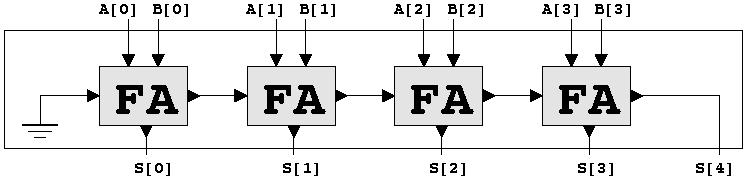
\includegraphics{adder.pdf}
  }
\caption{Addition of two integers (coded as bit vectors), using \emph{full adders.}\label{adder}}
\end{figure}

The following \alfa{} system describes a \emph{full adder}:
\index{full adder}
\begin{verbatim}
      system FullAdder (A,B,Cin : boolean) 
               returns (X,Cout : boolean);
      let
        X = A xor B xor Cin;
        Cout = (A and B) or (A and Cin) or (B and Cin);
      tel;
\end{verbatim}

To build an adder using this program, we need to 
instanciate a collection of such systems,
as shown in Fig.\ref{adder}. The shape of this collection may
be expressed as the {\alfa} domain \texttt{\{~b~|~0<=b<W~\}} where
\texttt{W} is a size parameter giving the number of bits of the
adder.
\index{use statement}
\index{use statement@\texttt{use}}

The \textbf{use} construct of {\alfa} allows precisely that. The
following system describes in {\alfa} the adder given in
Fig.~\ref{adder}:
\index{adder}
\index{binary addition}
\begin{verbatim}
system Plus: {W|W>1} (A,B: {b| 0<=b<W} of boolean)              -- 1       
             returns (S : {b| 0<=b<=W} of boolean);             -- 2       
var                                                             -- 3       
  Cin, Cout, X : {b| 0<=b<W} of boolean;                        -- 4       
let                                                             -- 5       
  Cin[b] =                                                      -- 6       
    case                                                        -- 7       
      {| b=0} : 0[];                                            -- 8       
      {| b>0} : Cout[b-1];                                      -- 9       
    esac;                                                       -- 10      
  use {b| 0<=b<W} FullAdder[] (A,B,Cin) returns(X, Cout);       -- 11      
  S[b] =                                                        -- 12      
    case                                                        -- 13      
      {| b<W} : X;                                              -- 14      
      {| b=W} : Cout[W-1];                                      -- 15      
    esac;                                                       -- 16      
tel;                                                            -- 17      
\end{verbatim}
In this system, line 11 reads as follows: 
\index{use statement}
\index{use statement@\texttt{use}}
\begin{quote}
"Use (or instantiate)
a collection of
instances of the subsystem \texttt{FullAdder}. This collection has the
shape of the extension domain\index{extension domain} 
\verb!{ b | 0<=b<W }! and is thus indexed
by index \texttt{b}. Let the inputs of the \texttt{b}-th instance be
the variables \texttt{A}, \texttt{B} and \texttt{Cin} at point
\texttt{b}, and similarly let the outputs of this collection of
instances be the variables \texttt{X} and \texttt{Cout}."
\end{quote}
Lines~6-10 describe the carry propagation, and lines~12-16
define the output of this binary adder.

\index{dimension extension}
In other words, line~11 is a shortcut for the following equations,
which are those of the system \texttt{FullAdder} whith the dimension
of the variables extended from zero to one:
\begin{verbatim}
        X[b] = A[b] xor B[b] xor Cin[b];
        Cout[b] = (A[b] and B[b]) or (A[b] and Cin[b]) or (B[b] and Cin[b]);
\end{verbatim}

\paragraph{Note.} In general, the extension indexes are 
added {\em to the left} of the existing indexes. This
cannot be seen in this example, since the full adder subsystem
has no indexes. 

\subsection{Handling structured programs}
A structured program is stored in {\mmalfa{}} as a {\mma{}} list of
systems called a \emph{library}. The default library is stored in the
global variable \verb!$library!.
\index{library}
\index{library@\texttt{\$library}}

A structured program may be written in one single file or several
distinct files.  In the former case the \texttt{load[]} function
returns a library composed of all the systems contained in the file,
and stores this library in \verb!$library!. %$ 
\index{load@\texttt{load}}

In addition, two functions, \texttt{putSystem[]} and
\texttt{getSystem[]}, may be used to get a system from a library
as the current system \texttt{\$result}\index{result@\texttt{\$result}}, and conversely
and to put back a modified system into a library. 
Typically a
system is extracted from the library as the {\em current}
system, modified by some program
transformation, and then put back in the library.
\index{putSystem@\texttt{putSystem[]}}
\index{getSystem@\texttt{getSystem[]}}

The commands to be used are \texttt{getSystem[]} and
\texttt{putSystem[]}.

\subsection{Program transformations associated with structures}

Most \mmalfa{} functions handle parameterized programs and \emph{use}
statements. There are, however, some major exceptions such as the
\texttt{cGen} translator\index{cGen@\texttt{cGen}} which generates code
only for {\em flat} {\Alpha} programs without subsystems. 
\mmalfa{}
provides functions to transform a structured program
into a flat equivalent one:
\begin{itemize}
\item \texttt{assignParameterValue[]}
\index{assignParameterValue@\texttt{assignParameterValue[]}}
gives a value to a size parameter, i.e. it refines a generic system
into a specialized one.
\item \texttt{inlineSubSystem[]}
\index{inlineSubSystem@\texttt{inlineSubSystem[]}}
expands a
\emph{use} statement, replacing it with the equations of the
corresponding subsystem, properly modified to take the dimension
extension into account.\index{flattening a structured program}
\item \texttt{inlineAll[]}
\index{inlining a subsystem}
\index{inlineAll@\texttt{inlineAll[]}}
recursively flattens a
structured {\alfa} program. \texttt{inlineAll[exceptions->\{sys\}]}
inlines all subsystems but those whose names appear in the 
exception list.
\end{itemize}

\paragraph*{More on subsystems}
For more information see 
{the subsystem documentation} in file
\begin{verbatim}
$MMALPHA/doc/Users/SubSystems.pdf
\end{verbatim}
If you are interested in scheduling structured subsystem, 
see an example in the \texttt{More} section of the 
\texttt{Master} notebook. 

\paragraph*{Troubleshouting}
There is a nasty bug in \texttt{inlineSubSystem} and
\texttt{inlineAll}. If you try to inline, with extension, 
a scalar equation, this equation must be given in 
standard notation, not in array notation. In Example~\ref{bug},
the equation in the called system must not be
written \texttt{out[] = 2[] + in[]}.
\begin{ex}{~}
\begin{verbatim}
system called (in: integer) returns (out: integer);
let
  -- This works
  out = 2.(->) + in;
tel;
system caller : {N | N>=1}
 (v: {i| 0< i <= N} of integer) 
 returns (w: {i| 0< i <= N} of integer);
let
  use {i| 0<i<=N} called (v) returns (w);
tel;
\end{verbatim}
\label{bug}
\end{ex}
\section{And now?}
\label{andnow}
In this document, we have presented a few possibilities of 
\mmalfa{}. You should now know if you are interested in 
using the \mmalfa{} software. 

If this is the case, you will find in the \alfa{} distribution 
some additional examples. See appendix~\ref{mmalphacontent}.

\bibliographystyle{alpha}
\bibliography{AlphaStart}

\newpage
\appendix
\section{Definition of \Alpha}
\label{alpha1}

\subsection{Meta Syntax}
\begin{tabbing}
xxxxxxx\= xxxxxxxxxxxxxxxxxx\= xxxxxxxxx\= xxxxxxx\= \kill
\>{\sl phrase* } \>===\>  zero or more repetitions of {\sl phrase}.\\
\> {\sl phrase1 {\sl \Alt} phrase2} \>===\> alternation, either {\sl
phrase1} or {\sl phrase2}.\\
\>  [\ldots] \>===\> optional phrase.\\
\> \Group{\ldots} \>===\> syntactic grouping.\\
\> {\bf \tt bold} \>===\> a terminal.\\
\> {\sl Italic} \>===\> a non-terminal.\\
\end{tabbing}

\subsection{Systems}
\Program{} stands for a library of \alfa{} programs. 
\PDecl{} (or \SystemDecl) is a single system. 
\Name{} is a system name. \ParamDecl{} is the declaration 
of a parameter domain. 
\InputDeclList{} is the list of input declarations. 
\OutputDeclList{} is the list of output declarations. 
\LocalDeclList{} is the list of local declarations. 
{\tt
\begin{tabbing}
xxxxxxxxxxxxxxxx\= xxx\= xx\=  xx\= \kill
\Program     \> :: \>\> \PDecl\ \PDecl *\\
\PDecl       \> :: \>\> \SystemDecl\\
\\\SystemDecl   \> :: \>\> system\ \Name \Opt{ : \ParamDecl }
                                    ( \InputDeclList )\\
\> \>\>\>  returns ( \OutputDeclList ) ;\\
\> \>\>\> \Opt{ var \LocalDeclList ;} \\
\> \>\>\> \EquationBlock ;\\
\\
\Name \>::\>\> \Identifier\\
\\
\ParamDecl  \> :: \>\> \Domain \\
\\
\InputDeclList \>::\>\> \VarDeclList\\
\OutputDeclList \>::\>\> \VarDeclList\\
\LocalDeclList \>::\>\> \VarDeclList\\
\end{tabbing}
}

\subsection{Declarations of variables}
\VarDeclList{} stands for a variable declaration. 
Notice that scalar types have been extended to 
special hardware types, such as 
\texttt{integer[S,10]} -- a signed
10 bit integer -- or
\texttt{integer[U,10]} -- an unsigned
10 bit integer. 
{\tt
\begin{tabbing}
xxxxxxxxxxxxxxxx\= xxx\= xx\=  xx\= \kill
\VarDeclList \>::\>\> \VarDeclaration *\\
\VarDeclaration \>::\>\> \IdentifierList\ : \Opt{\Domain of} \ScalarType ;\\
\ScalarType \> ::\>\> integer \Alt\ real \Alt\ boolean
\end{tabbing}
}

\subsection{Domains}
\Domain{} stands for a domain declaration. \IndexList{} is
a list of indexes, and \ConstraintList{} a list of constraints. 

Notice that operations on domains such as intersection
(\texttt{\&}), union (\texttt{|}), complement (\texttt{~}) and
preimage by an affine function are allowed. The parser 
does the corresponding operation. 

I am not sure that the \texttt{convex} syntax, nor the 
domain expressions fully work...

\ConstraintList{} is a list of constraints, each one being an
increasing constraint, a decreasing constraint, or an 
inequality.
{\tt
\begin{tabbing}
xxxxxxxxxxxxxxxx\= xxx\= xx\=  xx\= \kill
\Domain \>::\>\> \{ \IndexList \verb~|~ \ConstraintList \}\\
\>\>\Alt\> \Domain \verb~|~ \Domain\\
\>\>\Alt\> \Domain \verb~&~ \Domain\\
\>\>\Alt\> \Domain .\AffineFunction\\
\>\>\Alt\> \verb'~' \Domain\\
\>\>\Alt\> \Domain .convex\\
\>\>\Alt\> ( \Domain )\\
\\
\IndexList\>::\>\> \Opt{\IndexList ,} \Identifier\\
\\
\ConstraintList\>::\>\> \Opt{\ConstraintList ;} \Constraint\\
\Constraint \>::\>\> \IncreasingSeq \Alt\ \DecreasingSeq \Alt\ \EqualitySeq\\
\IncreasingSeq \>::\>\> \Group{ \IncreasingSeq \Alt\ \IndexExpList }
  \Group{ < \Alt\ <= } \IndexExpList\\
\DecreasingSeq \>::\>\> \Group{ \DecreasingSeq \Alt\ \IndexExpList }
  \Group{ > \Alt\ >= } \IndexExpList\\
\EqualitySeq\>::\>\> \Group{ \EqualitySeq \Alt\ \IndexExpList } = \IndexExpList
\end{tabbing}
}

\subsection{Equations}
\EquationBlock{} is the block of equation declarations. 
\Equation{} represents an equation, which can be either 
in array notation (when the lhs has the form \texttt{var[...]})
or in standard notation. An equation can also be a \texttt{use} statement.
\footnote{I am not sure of the syntax for the 
paramAssignation with the dot...}

{\tt
\begin{tabbing}
xxxxxxxxxxxxxxxx\= xxx\= xx\=  xx\= \kill
\EquationBlock \>::\>\> let \EquationList tel \\
\EquationList  \>::\>\> \Opt{ \EquationList } \Equation\\
\Equation\>::\>\> \Identifier [ \IndexList ] = \Expression ;\\
\>\> \Alt\ \> \Identifier = \Expression ;\\
\>\> \Alt\ \> use \Opt{ \ExtensionDomain} \Identifier
                                    \Opt{.\ParamAssignation} \\
\>\>\>\>( \InputList )\\
\>\>\>\> returns ( \IdentifierList ) ;\\
\\
\ParamAssignation \>::\>\> \AffineFunction \\
\\
\InputList \>::\>\> \Opt{ \InputList , } \Expression\\
\\
\ExtensionDomain \>::\>\> \Domain \\
\end{tabbing}
}

\subsection{Expressions}
Expressions can be case expressions, if statements\footnote{\alfa{}
conditional statements are strict, that is to say, both branches
are evaluated, and moreover, the domain of the statement is 
the intersection of that of the condition and of the 
expressions.}, restrictions, affine dependencies, binary operations, 
unary operations, and reductions\footnote{Reductions are allowed, 
but few transformations are currently available.}
{\tt
\begin{tabbing}
xxxxxxxxxxxxxxxx\= xxx\= xx\=  xx\= \kill
\Expression\>::\>\> case \ExpressionList esac \\
\>\> \Alt\ \> if \Expression then \Expression else \Expression\\
\>\> \Alt\ \> \Domain :\Expression\\
\>\> \Alt\ \> \Expression .\AffineFunction\\
\>\> \Alt\ \> \Expression [ \IndexExpList ] \\
\>\> \Alt\ \> \Expression \BinaryOp \Expression\\
\>\> \Alt\ \> \BinaryOp ( \Expression, \Expression ) \\
\>\> \Alt\ \> \UnaryOp \Expression\\
\>\> \Alt\ \> reduce ( \CommutativeOp, \AffineFunction, \Expression ) \\
\>\> \Alt\ \> ( \Expression ) \\
\>\> \Alt\ \> \Identifier\\
\>\> \Alt\ \> \Constant\\
\\
\ExpressionList \>::\>\> \Opt{ \ExpressionList  } \Expression ;\\
\\
\BinaryOp \>::\>\> \CommutativeOp \Alt\ \RelativeOp \Alt\ - \Alt\ div \Alt\ mod\\
\CommutativeOp \>::\>\> + \Alt\ * \Alt\ / \Alt\ and \Alt\ or \Alt\ xor \Alt\ min \Alt\ max\\
\RelativeOp \>::\>\> = \Alt\ <> \Alt\ < \Alt\ <= \Alt\ > \Alt\ >=\\
\UnaryOp \>::\>\> - \Alt\ not \Alt\ sqrt\\
\\
\Constant \>::\>\> \IntegerConstant \Alt\ \RealConstant \Alt\ \BooleanConstant\\
\end{tabbing}
}
\subsection{Dependance Functions and Index Expressions}
\AffineFunction{} stands for affine functions. 
{\tt
\begin{tabbing}
xxxxxxxxxxxxxxxx\= xxx\= xx\=  xx\= \kill
\AffineFunction \>::\>\> ( \IndexList -> \IndexExpList )\\
\IndexExpList \>::\>\> \Opt{ \IndexExpList, } \IndexExpression\
          \Alt\ \IndexExpression\\
\IndexExpression \>::\>\> \IndexExpression \Group{+ \Alt\  - } \IndexTerm\
          \Alt\ [ - ] \IndexTerm\\
\IndexTerm \>::\>\> \IntegerConstant \Identifier \Alt\ \IntegerConstant \Alt\ \Identifier
\end{tabbing}
}


\subsection{Terminals}
{\tt
\begin{tabbing}
xxxxxxxxxxxxxxxx\= xxx\= xx\=  xx\= \kill
\IntegerConstant \>::\>\> \Opt{-} \Number\\
\RealConstant \>::\>\> \Opt{-} \Number .\Number\\
\BooleanConstant \>::\>\> true \Alt\ false \Alt True \Alt\ False\\
\Number \>::\>\> \Digit \Digit *\\
\Digit \>::\>\> 0 \Alt\ 1 \Alt\ldots\Alt\ 9\\
\Identifier \>::\>\> \Letter \Group{\Letter \Alt\ \Digit} *\\
\Letter \>::\>\> a \Alt\ldots\Alt\ z  \Alt\ A \Alt\ldots\Alt\ Z \Alt\ \verb'_'\\
\end{tabbing}
}
Note: avoid using underscores...

\section{Description of the internal format of ASTs}
\label{ast}
This section describes the format of Abstract Syntax Trees (AST) of
\alfa{} programs, as handled by \mma{}. In other words, 
the AST of a program is the \mma{} expression that \MMAlfa{} stores in 
variable \texttt{\$result} when the \texttt{load} command is 
executed. It can be displayed just by having \mma{} evaluate
the expression \texttt{\$result}.

In the following description, non terminals are
written inside angle brackets \verb\<>\.  
For readability, keywords are
written without the prefix \texttt{Alpha`} which is implicit. 
For example, the keyword \texttt{system} is actually represented
by the symbol \texttt{Alpha`system}. 
The documentation is presented in
five sections: Systems, Domains, Equations, Matrices and General.

\subsection{Systems}
\begin{verbatim}
   <library>       ::= {<system> , ... , <system>} 
   <system>        ::= system [ <system_id>,
                                <param_space>, 
                                <in_var>, 
                                <out_var>,
                                <local_var>, 
                                <equation_list> ]
   <param_space>::= <domain>
   <in_var>     ::= <declare_list>
   <out_var>    ::= <declare_list>
   <local_var>  ::= <declare_list>
   <declare>    ::= decl [ <id>, <data_type>, <domain> ]
   <data_type>  ::= integer | boolean | real | notype
\end{verbatim}

\subsection{Domains}
The domain specification closely follows the internal format of the domain
definition in the domain library. This was done to minimize the overhead of
domain storage and of making library calls.  In Mathematica, domains should
only be changed by making calls to the domain library.

\begin{verbatim}
   <domain>     ::= domain [ <dimension_number>,
                             <id_list>, 
                             <polyhedron_list> ] 
   <polyhedron> ::= pol [ <constraints_number>, 
                          <rays_number>,
                          <equations_number>, 
                          <lines_number>,
                          <constraint_list>, 
                          <ray_list> ] 
   <constraint> ::= { <const_type>, 
                      <number>, ... , <number> }
   <const_type> ::= 0 | 1
                    0 / 1 = constraint is equality / inequality
   <ray>        ::= { <ray_type>, 
                      <number>, ... , <number> }
   <ray_type>   ::= 0 | 1
                    0 / 1 = ray is line / ray
\end{verbatim}

\subsection{Equations}
\begin{verbatim}
   <equation>   ::= equation [ <id>, <exp> ]
                  | use [ <id>, 
                          <extension>, 
                          <param_assign>, 
                          <exp_list>,
                          <id_list> ]
   <extension>  ::= <domain>
   <param_assign> ::= <matrix>

   <exp>        ::= var[<id>]
                  | const[<number>] | const[<boolean>] | const[<real>]
                  | binop [ <bop>, <exp>, <exp> ]
                  | unop  [ <uop>, <exp> ]
                  | if [ <exp>, <exp>, <exp> ]
                  | affine [ <exp>, <matrix> ]
                  | restrict [ <domain>, <exp> ]
                  | case [ <exp_list> ]
                  | call [ <id>, <exp_list> ]
                  | reduce [ <casop>, <matrix>, <exp> ]
   <bop>        ::= add | sub | mul | div | idiv | mod | min | max
                  | eq | le | lt | gt | ge | ne | or | and | xor
   <unop>       ::= neg | not | sqrt 
   <casop>      ::= add | mul | and | or | xor | min | max
\end{verbatim}

\subsection{Matrices}
\begin{verbatim}
   <matrix>     ::= matrix [ <rows_number>,
                             <cols_number>, 
                             <id_list>, 
                             { { <number>, <number>, ... , <number> },
                               { <number>, <number>, ... , <number> },
                               ...
                               { <number>, <number>, ... , <number> } } ]
\end{verbatim}

\subsection{General specifications}
Numbers, ids, and lists, as used above, are defined generally
(with \verb\<*>\ representing any nonterminal ).

\begin{verbatim}
   <*_number>   ::= <number>
   <*_id>       ::= <id>
   <*_list>     ::= { <*>, <*>, ... , <*> }

   <number>     ::= [0-9][0-9]* | Infinity
   <real>       :=  <number>.<number>
   <boolean>    ::= True | False
   <id>         ::= "a name"
   <comment>    ::= (* blah blah blah *)
\end{verbatim}

\texttt{Reserved Keywords}

\begin{verbatim}
        Alpha`add       Alpha`affine    Alpha`and       Alpha`binop
        Alpha`boolean   Alpha`call      Alpha`case      Alpha`const
        Alpha`decl      Alpha`div       Alpha`domain    Alpha`eq
        Alpha`equation  Alpha`ge        Alpha`gt        Alpha`idiv
        Alpha`if        Alpha`integer   Alpha`le        Alpha`lt
        Alpha`matrix    Alpha`max       Alpha`min       Alpha`mod
        Alpha`mul       Alpha`ne        Alpha`neg       Alpha`not
        Alpha`notype    Alpha`or        Alpha`pol       Alpha`real
        Alpha`reduce    Alpha`restrict  Alpha`sqrt      Alpha`sub
        Alpha`system    Alpha`unknown   Alpha`unop      Alpha`use
        Alpha`var       Alpha`xor
\end{verbatim}

\section{A brief description of the \MMAlfa{} distribution}
\label{mmalphacontent}

\subsection{The \texttt{Master} notebook}
The master notebook is open by the \texttt{start[]} 
command. It contains 6 sections.
\begin{itemize}
\item The welcome section. 
\item The introduction notebooks: the 
\texttt{getting-started}\index{getting-started@The \texttt{Getting-started} notebook}
notebook, and the \texttt{mma-intro}\index{mma-intro@The \texttt{mma-intro} notebook}
notebook. 
\item The simple examples section. It contains pointers to the 
matrix-vector, the Fir filter, the Fifo, and the delay line 
demonstrations. 
\item The advances examples section. Here are presented a demonstration
of the Delayed Least-Mean Square filter, of the structured scheduler, 
and of the Samba architecture for DNA sequence alignment.
\footnote{Do the DLMS... Check the structured scheduler...}
\item More contains an access to the Domlib notebook, and some
suggestion about the organization of your own notebooks. It 
explained how you can set the variables \texttt{\$myNotebooks},
\texttt{\$myMasterNotebook}, then use the \texttt{myStart[]} 
and the \texttt{link}
commands to access directly your own working space. 
\item Finally, the Tests section gives access to a test notebook. 
\end{itemize}

\subsection{Documentation}
To explore the \MMAlfa{} distribution, you can follow the 
html files which are in each subdirectory of the distribution.
The structure of 
the distribution is as follows. The main directory is called \MMAlfa{}. It
contains another directory called Mathematica which is the 
\MMAlfa{} distribution properly speaking. In the \MMAlfa{} directory, 
the file \texttt{welcome.html} gives access to the documentation. 

The Mathematica directory is organized as follows:
\begin{itemize}
\item \texttt{bin.cygwin} and \texttt{bin.solaris} 
directories contain the binary files for execution of \MMAlfa{} on 
the Windows NT and Solaris system respectively. 
\item \texttt{config} contains the configuration files.
\item \texttt{demos} contains the demonstrations notebooks.
\item \texttt{doc} contains the documentation notebooks.
\item \texttt{lib} contains the Mathematica packages which form 
\MMAlfa{}.
\item \texttt{sources} contains the source files of the \C{} programs
and of the latex documentation files. 
\item \texttt{tests} containes the test programs for \MMAlfa{}.
\end{itemize}

\printindex

\newpage
\tableofcontents


\end{document}
%
% File created on {2007, 11, 15, 17, 10, 20.779597} by makeDoc.
%
% Section header
\section{The Alpha`Vhdl2` package } 
\label{label:Alpha`Vhdl2`}
\alphausage{Vhdl2}{Alpha`Vhdl2` contains the Vhdl generator. The main function is a2v.}{Alpha/Vhdl2.m}{Alpha`Vhdl2`}
\index{Vhdl2}

\alphausage{\$vhdlCurrent}{vhdlCurrent is a global variable owned by Vhdl, which contains the  current program}{Alpha/Vhdl2.m}{Alpha`Vhdl2`}
\index{\$vhdlCurrent}

\alphausage{\$vhdlOutputFile}{}{Alpha/Vhdl2.m}{Alpha`Vhdl2`}
\index{\$vhdlOutputFile}

\alphausage{a2v}{a2v[] translates in Vhdl all the files contained in \$library.  a2v[lib] translates in Vhdl all the files contained in library lib. a2v[sys] translates in Vhdl the system sys. a2v has many  options (see Options[a2v]). a2v[elem,tinit] runs a2v on library or system elem, and fixes the initial value of the time to the integer value tinit.}{Alpha/Vhdl2.m}{Alpha`Vhdl2`}
\index{a2v}

\alphausage{bitWidth}{bitWidth[sys,var] gives the bit width of variable var. Default  value of sys is \$result.}{Alpha/Vhdl2.m}{Alpha`Vhdl2`}
\index{bitWidth}

\alphausage{bitWidthOfExpr}{bitWidth[sys,expr] gives the bit width of an expression. Default of sys is \$result.}{Alpha/Vhdl2.m}{Alpha`Vhdl2`}
\index{bitWidthOfExpr}

\alphausage{getVhdlType}{getVhdlType[sys,var] return the vhdl type of the element of array var}{Alpha/Vhdl2.m}{Alpha`Vhdl2`}
\index{getVhdlType}

\alphausage{showVhdl}{showVhdl[] prints the Vhdl generated for the system in \$result.  showVhdl[s] show the content of the file s.vhd.}{Alpha/Vhdl2.m}{Alpha`Vhdl2`}
\index{showVhdl}

\alphausage{stim}{stim[] post processes all the simuli files (replace blanks by zeros).  These files are generated from a C code in hexadecimal and there is no  format in C to write zeros in for the first digits.}{Alpha/Vhdl2.m}{Alpha`Vhdl2`}
\index{stim}


%
% File created on {2007, 11, 15, 17, 10, 20.994002} by makeDoc.
%
% Section header
\section{The Alpha`VhdlTestBench` package } 
\label{label:Alpha`VhdlTestBench`}
\alphausage{VhdlTestBanch}{Package,contains definition of funtion for generating test benches for VHDL generated from Alphard}{Alpha/VhdlTestBench.m}{Alpha`VhdlTestBench`}
\index{VhdlTestBanch}

\alphausage{vhdlTestBenchGen}{vhdlTestBenchGen[sys] generates a VHDL test bench for  the VHDL component generated from sys with the a2v command. sys mustbe a valid Alphard system, it works if sys is a cell, a module or a controller (not an interface), as for a2v, the parameters must be assigned. vhdlTestBenchGen[] applies on \$result}{Alpha/VhdlTestBench.m}{Alpha`VhdlTestBench`}
\index{vhdlTestBenchGen}

\alphausage{mkVhdlLoop}{test}{Alpha/VhdlTestBench.m}{Alpha`VhdlTestBench`}
\index{mkVhdlLoop}

\alphausage{mkVhdlLowerBound}{test}{Alpha/VhdlTestBench.m}{Alpha`VhdlTestBench`}
\index{mkVhdlLowerBound}

\alphausage{mkVhdlUpperBound}{test}{Alpha/VhdlTestBench.m}{Alpha`VhdlTestBench`}
\index{mkVhdlUpperBound}



\chapter{Utilities}
\label{utilities}
%
% File created on {2008, 3, 11, 15, 1, 57.629758} by makeDoc.
%
% Section header
\section{The Alpha`MakeDoc` package } 
\label{label:Alpha`MakeDoc`}
\subsection{Note regarding the documentation of \MMAlfa{}}
\label{doc-makedoc}
The \MMAlfa{} software is (partially) documented in various
ways.\footnote{This chapter has been
proof-read by Patrice Quinton on January 8, 2007.}
\begin{itemize}
\item A \texttt{html} documentation is included in the distribution.
It can be accessed from the \texttt{welcome.html} file in the 
\texttt{\$MMalpha{}} directory. 
\item A {\em getting started} document is available in form of
a \texttt{pdf}
file. It is accessible from the initial \texttt{html} welcome
page and is located in:
\begin{verbatim} 
$MMAlpha/doc/QuickStart/AlphaStart.pdf
\end{verbatim} 
This document is the most up-to-date tutorial for \MMAlpha{}. It does not
describe all features of \MMAlpha{}, but normally, allows a user to
discover the main features of the software.
\item A reference manual is being developped in:
\begin{verbatim} 
$MMAlpha/doc/ReferenceManual
\end{verbatim}
and it is described hereafter.
\item Other documentation files exist, but they are not guaranteed to 
be up-to-date.
\end{itemize}

The reference manual of \MMALPHA{} is obtained through the use 
of commands in the \texttt{Makedoc} package. 
It is produced by executing the program called \texttt{genReferenceManual.m}
which is situated in the same directory.

This program contains a set of calls to the function \texttt{doDoc}
of the \texttt{Makedoc} package (see \texttt{?doDoc}). Each one of
these calls reads a package -- for example, \texttt{Alpha/Makedoc.m} --
whose name is relative to directory
\begin{verbatim} 
$MMALPHA/lib/Packages
\end{verbatim}
and translates it into a \LaTeX{} file -- for example, \texttt{Makedoc.tex}, --
in target directory \texttt{\$MMALPHA/doc/ReferenceManual}.

The reference manual itself is edited manually. It is in the 
file:
\begin{verbatim}
referenceManual.tex
\end{verbatim}
of the same directory. It contains
basically input statements for the documentation files created by 
\texttt{doDoc}. This function (which is documented hereafter), has
several options: one can either generate a standalone \LaTeX{} file, or
an input file (this helps for editing the documentation), one can 
specify a list of functions that are only to be documented, one can 
specify where the file has to be put, etc. 

The reference manual is based on the usage and note statements which are
contained in a given package. In there exists a file named 
\texttt{incl-textFile} in the target directory, then an include 
statement for this file is added in the generated \LaTeX{} file.
For example, the documentation that you are reading is in the 
file \texttt{incl-Makedoc.text} file, in directory:
\begin{verbatim}
$MMALPHA/doc/referenceManual
\end{verbatim}
Therefore, when the 
\texttt{Makedoc.m} file is processed by the corresponding 
statement in the \texttt{genReferenceManual.m} program, i.e.:
\begin{small}
\begin{verbatim}
doDoc["Alpha/MakeDoc.m", "MakeDoc.tex", 
  targetDir -> Environment["MMALPHA"] <> "/doc/ReferenceManual"];
\end{verbatim}
\end{small}
an input statement is included in the \texttt{Makedoc.tex} file 
which is generated.

The \texttt{doDoc} function tries to modify the content of the
usage and note statements so that special symbols are correctly
output in \LaTeX{}. These transformations are described in the
variable \texttt{repRules} of the package, and may be modified. 
Index statements are generated for each usage statement. 


\alphausage{MakeDoc}{MakeDoc is a package which contains functions for the automatic creation of a reference Manual. MakeDoc contains functions doDoc and makeDoc.}{Alpha/MakeDoc.m}{Alpha`MakeDoc`}
\index{MakeDoc}

\alphanote{MakeDoc}{Functions of MakeDoc read all usage and note statements of a package, and for each one, they produce a Latex macro entry alphausage or alphanote. Before creating an entry, substitutions are performed on the text, so that special words (such as \$schedule) and special characters (such as \_) are transformed. The substitution list is in the private variable repRules in the file MakeDoc.m.} 
 
\alphausage{doDoc}{doDoc[ package, texFile ] generates in file texFile the documentation LaTex file associated to a Mathematica file package. doDoc extracts the information contained in the usage and note descriptions placed at the beginning of file package, and produces an output Latex file. doDoc[ package ] automatically writes in a file which has the name  package where the .m suffix is replaced by .tex.  doDoc[ Package, functionList ] generates the documentation only for  the functions enumerated in functionList (as Strings). doDoc has  options fullLatex and callFile which allow a complete latex file,  resp. a calling Latex file to be produced. If there exists a file incl-textFile in the target directory, then a Latex input statement is added in the documentation package.}{Alpha/MakeDoc.m}{Alpha`MakeDoc`}
\index{doDoc}

\alphausage{fullLatex}{fullLatex is an option of doDoc and makeDoc. Default value is False. If True, the latex file contains the preamble and the \\end\{document\} statement.  Otherwise, it should be used in an input file}{Alpha/MakeDoc.m}{Alpha`MakeDoc`}
\index{fullLatex}

\alphausage{targetDir}{option of doDoc. By default, it is "". Gives the name of a directory where the latex file and the calling latex file should be written.}{Alpha/MakeDoc.m}{Alpha`MakeDoc`}
\index{targetDir}

\alphausage{callFile}{callFile is an option of doDoc and makeDoc. Default valus is False. If True, a latex calling file is created.}{Alpha/MakeDoc.m}{Alpha`MakeDoc`}
\index{callFile}

\alphausage{sourceDir}{option of makeDoc. Default value is Null. If Null, the source package are those of \$MMALPHA. Their names are in the file \$MMALPHA/sources/ MaleDoc/List\_modules. Otherwise, these names are prefixed by the  value of the sourceDir option.}{Alpha/MakeDoc.m}{Alpha`MakeDoc`}
\index{sourceDir}

\alphausage{makeDoc}{This function does not work, currently. Use doDoc instead. makeDoc[] updates the Reference Manual of \MMAlpha{} by running  the file genReferenceManual.m in directory\\ \$MMALPHA/doc/ReferenceManual/\\ This produces new versions of the latex files describing the  packages. The Reference Manual can be produced using Latex on  referenceManual.tex. See also doDoc.}{Alpha/MakeDoc.m}{Alpha`MakeDoc`}
\index{makeDoc}

%Proof-read

\chapter{Add-ons}
%
% File created on {2007, 11, 15, 17, 10, 19.944972} by makeDoc.
%

%
% File created on {2007, 11, 15, 17, 10, 19.948099} by makeDoc.
%

%
% File created on {2004, 7, 31, 14, 57, 0} by makeDoc.
%

%
% File created on {2007, 11, 15, 17, 10, 21.041330} by makeDoc.
%

%
% File created on {2007, 11, 15, 17, 10, 19.106120} by makeDoc.
%
% Section header
\section{The Alpha`INorm` package } 
\label{label:Alpha`INorm`}
\alphausage{iNorm}{iNorm[s:\_system, k:\_Integer, options] computes the  imperative form of system s. k is the dimension of time. As usual,  iNorm[k, options] means \$result = iNorm[\$result, k, options]. See  Options[iNorm] for options.}{Alpha/INorm.m}{Alpha`INorm`}
\index{iNorm}

\alphausage{rnf}{rnf[s:\_system] returns the R normal form of s.}{Alpha/INorm.m}{Alpha`INorm`}
\index{rnf}


%
% File created on {2007, 11, 15, 17, 10, 20.227042} by makeDoc.
%

%
% File created on {2007, 11, 15, 17, 10, 21.043002} by makeDoc.
%
% Section header
\section{The Alpha`Lexicographic` package } 
\label{label:Alpha`Lexicographic`}
\alphausage{domLexGreater}{domLexGreater[v:\_Matrix] returns a domain D such that for all z in D, z$>$v, where $>$ means lexicographically greater. V is a parametrized vertex. If v is a n*(p+1) matrix, D is a n+p domain, and the p last dimensions are parameter dimensions. Example: domLexGreater[\{\{1,0\},\{0,2\}\}] returns \{a,b,c $|$ c+1$<$=a\} $|$ \{a,b,c $|$ a=c; 3$<$=b\}, where c is the parameter index. domLexGreater[v:\_Vector] is a shortcut for 0-dimensional parameter space. (i.e. domLexGreater[\{0,0,1\}] means domLexGreater[\{\{0\},\{0\},\{1\}\}].}{Alpha/Lexicographic.m}{Alpha`Lexicographic`}
\index{domLexGreater}

\alphausage{domLexLower}{domLexLower[v:\_Matrix] returns a domain D such that for all z in D, z$<$v, where $<$ means lexicographically lower. V is a parametrized vertex. If v is a n*(p+1) matrix, D is a n+p domain, and the p last dimensions are parameter dimensions. Example: domLexLower[\{\{1,0\},\{0,2\}\}] returns \{a,b,c $|$ a$<$=c-1\} $|$ \{a,b,c $|$ a=c; b$<$=1\}, where c is the parameter index. domLexLower[v:\_Vector] is a shortcut for 0-dimensional parameter space. (i.e. domLexLower[\{0,0,1\}] means domLexGreater[\{\{0\},\{0\},\{1\}\}].}{Alpha/Lexicographic.m}{Alpha`Lexicographic`}
\index{domLexLower}

\alphausage{lexGreaterQ}{lexGreaterQ[a:\_Matrix, b:\_Matrix, p:\_domain] returns True  if a is lexicographicallygreater than b for any value of parameters in p. a and b  are parametrized vectors.}{Alpha/Lexicographic.m}{Alpha`Lexicographic`}
\index{lexGreaterQ}

\alphausage{lexGreaterOrEqualQ}{lexGreaterOrEqualQ[a:\_Matrix, b:\_Matrix, p:\_domain] returns True if a is lexicographically greater or equal than b for any value of parameters in p. a and b are parametrized vectors.}{Alpha/Lexicographic.m}{Alpha`Lexicographic`}
\index{lexGreaterOrEqualQ}

\alphausage{lexLowerQ}{lexLowerQ[a:\_Matrix, b:\_Matrix, p:\_domain] returns True  if a is lexicographically lower than b for any value of parameters in p. a and b  are parametrized vectors.}{Alpha/Lexicographic.m}{Alpha`Lexicographic`}
\index{lexLowerQ}

\alphausage{lexLowerOrEqualQ}{lexLowerOrEqualQ[a:\_Matrix, b:\_Matrix, p:\_domain] returns True if a is lexicographically lower or equal than b for any value of parameters in p. a and b are parametrized vectors.}{Alpha/Lexicographic.m}{Alpha`Lexicographic`}
\index{lexLowerOrEqualQ}


%
% File created on {2007, 11, 15, 17, 10, 21.053070} by makeDoc.
%

%
% File created on {2008, 3, 11, 16, 16, 25.885021} by makeDoc.
%
% Section header
\section{The Alpha`Matrix` package } 
\label{label:Alpha`Matrix`}
\alphanote{Matrix}{Documentation revised on March 11, 2008} 
 
\alphausage{Matrix}{The Alpha`Matrix` package contains a few functions related to Alpha matrices. These functions are  alphaToMmaMatrix, composeAffines, convHull, convexize, convexizeAll, deleteColumn, deleteRow, determinant, dropColumns, dropParameters,  dropRows, emptyLinearPartQ, getLinearPart, getTranslationVector,  hermite, hermiteL, hermiteR, inverseMatrix, identityQ, idLinearPartQ, idMatrix, inverseInContext, nullSpaceVectors, mmaToAlphaMatrix,  nullLinearPartQ, simplifyAffines, solveDiophantine, smithNormalForm,  squareMatrixQ, suppressRowNum, translationMatrix, translationQ, unimodularQ,  composeAffines, inverseMatrix, unimodularQ, unimodularCompletion,  unimodCompl.}{Alpha/Matrix.m}{Alpha`Matrix`}
\index{Matrix}

\alphausage{addLinSpace}{Obsolete function, replaced by the generalized ChangeOfBasis.}{Alpha/Matrix.m}{Alpha`Matrix`}
\index{addLinSpace}

\alphausage{alphaToMmaMatrix}{alphaToMmaMatrix[mat] translates a linear function from Alpha format into Mathematica format (list of list). If the linear function mat was affine (non nul constant part) this constant part is lost.  \\ Example:\\ alphaToMmaMatrix[\\ matrix[3, 3, \{i, j\}, \{\{1, 2, 0\}, \{0, 3, 0\}, \{0, 0, 1\}\}]\\ ]\\ gives \{\{1, 2\}, \{0, 3\}\}.}{Alpha/Matrix.m}{Alpha`Matrix`}
\index{alphaToMmaMatrix}

\alphausage{canonicalProjection}{Obsolete. canonicalProjection[dom, pos] returns a projected domain obtained  by supressing the indices given by the integer list pos.}{Alpha/Matrix.m}{Alpha`Matrix`}
\index{canonicalProjection}

\alphanote{canonicalProjection}{OBSOLETE. Replaced by (generalized) ChangeOfBasis.} 
 
\alphausage{composeAffines}{composeAffines[m1,m2] returns the composition of two affine matrices m1 and m2. These matrices are described in the Alpha format.}{Alpha/Matrix.m}{Alpha`Matrix`}
\index{composeAffines}

\alphausage{convHull}{convHull[ldom] returns the convex hull of a (possibly empty) list of  domains ldom.}{Alpha/Matrix.m}{Alpha`Matrix`}
\index{convHull}

\alphanote{convHull}{If the input list is empty, returns an empty list.} 
 
\alphausage{convexize}{convexize[domain] returns the convex hull of domain if domain is convex, otherwise returns domain unmodified. Used to convexize a union  of domains (try to use DomConvex instead).}{Alpha/Matrix.m}{Alpha`Matrix`}
\index{convexize}

\alphausage{convexizeAll}{convexizeAll[sys] tries to convexize all the non-convex domains of sys (default \$result) and returns the modified system.}{Alpha/Matrix.m}{Alpha`Matrix`}
\index{convexizeAll}

\alphausage{deleteColumn}{deleteColumn[m,k] removes the k-th column of the Alpha matrix m. It removes also index k of m.}{Alpha/Matrix.m}{Alpha`Matrix`}
\index{deleteColumn}

\alphausage{deleteRow}{deleteRow[m,k] removes the k-th row of the Alpha matrix m. It does not touch the index list of m.}{Alpha/Matrix.m}{Alpha`Matrix`}
\index{deleteRow}

\alphausage{determinant}{determinant[m] gives the determinant of a square Alpha matrix. The result can be integer or rationnal, the constant part is not taken into account.}{Alpha/Matrix.m}{Alpha`Matrix`}
\index{determinant}

\alphausage{dropColumns}{dropColumns[m,n] removes n columns of the Alpha matrix m, from front if n is positive, from end if n is negative. This function does not touch the  dimensions nor the indexes of the matrix.}{Alpha/Matrix.m}{Alpha`Matrix`}
\index{dropColumns}

\alphausage{dropParameters}{dropParameters[sys,m] removes the rows of Alpha matrix m corresponding to  parameters of system sys (default \$result). If there are too many  parameters, dropParameters returns m unchanged.}{Alpha/Matrix.m}{Alpha`Matrix`}
\index{dropParameters}

\alphausage{dropRows}{dropRows[m,n] removes n rows of the Alpha matrix m, from front if n is  positive, from the end otherwise. This function does not touch the  dimensions nor the indexes of the matrix.}{Alpha/Matrix.m}{Alpha`Matrix`}
\index{dropRows}

\alphausage{emptyLinearPartQ}{emptyLinearPartQ[m] is True if the linear part of matrix m is empty,  False otherwise.}{Alpha/Matrix.m}{Alpha`Matrix`}
\index{emptyLinearPartQ}

\alphausage{getLinearPart}{getLinearPart[m] returns the linear part of an affine function m.}{Alpha/Matrix.m}{Alpha`Matrix`}
\index{getLinearPart}

\alphausage{getTranslationVector}{getTranslationVector[m] returns the translation vector of a square  affine function m.}{Alpha/Matrix.m}{Alpha`Matrix`}
\index{getTranslationVector}

\alphausage{hermite}{hermite[m] returns the left hermite decomposition \{h,u\} (as Alpha matrices) of m1 (such that m1=composeAffines[h,u]).\\ WARNING: Currently, this function only deals with linear function (the constant part is ignored).}{Alpha/Matrix.m}{Alpha`Matrix`}
\index{hermite}

\alphausage{hermiteL}{hermiteL[m] performs the left Hermite decomposition of the Mathematica matrix m and returns mathematica matrices  \{H,Q\} where Q unimodular, H upper triangular and m = Dot[H,Q].}{Alpha/Matrix.m}{Alpha`Matrix`}
\index{hermiteL}

\alphausage{hermiteR}{hermiteR[m] computes the right Hermite decomposition of the  Mathematica matrix m and returns Mathematica matrices \{H,Q\}, where Q is unimodular, H is lower triangular, and m=Dot[Q,H].}{Alpha/Matrix.m}{Alpha`Matrix`}
\index{hermiteR}

\alphausage{inverseMatrix}{inverseMatrix[m] computes and returns the inverse of a square affine  matrix m.}{Alpha/Matrix.m}{Alpha`Matrix`}
\index{inverseMatrix}

\alphausage{identityQ}{identityQ[m] is True if an Alpha affine function m is the identity,  False otherwise.}{Alpha/Matrix.m}{Alpha`Matrix`}
\index{identityQ}

\alphausage{idLinearPartQ}{idLinearPartQ[m] is True if the linear part of the affine function given as Alpha matrix m is the identity, False otherwise.}{Alpha/Matrix.m}{Alpha`Matrix`}
\index{idLinearPartQ}

\alphausage{idMatrix}{idMatrix[idx\_List,idy\_List] returns the transformation matrix for dependence (idx$ \rightarrow $idy), where idx and idy are lists of index names. It is assumed that names in idy are also in idx.  \\Example:\\ idMatrix[\{"i","j"\},\{"i","i","j"\}] = \\ matrix[4, 3, \{"i","j"\}, \{\{1,0, 0\}, \{1, 0, 0\}, \{0, 1, 0\}, \{0, 0, 1\}\}].}{Alpha/Matrix.m}{Alpha`Matrix`}
\index{idMatrix}

\alphausage{inverseInContext}{inverseincontext[m,d] computes the inverse matrix of Alpha matrix m in  context with domain d, i.e., taking into account the lineality space  defined by d.}{Alpha/Matrix.m}{Alpha`Matrix`}
\index{inverseInContext}

\alphausage{isIdLinearPart}{obsolete form of idLinearPartQ.}{Alpha/Matrix.m}{Alpha`Matrix`}
\index{isIdLinearPart}

\alphausage{isNullLinearPart}{obsolete form of nullLinearPartQ.}{Alpha/Matrix.m}{Alpha`Matrix`}
\index{isNullLinearPart}

\alphausage{nullSpaceVectors}{nullSpaceVectors[mat] gives the list of vectors of the null space of Alpha matrix mat.}{Alpha/Matrix.m}{Alpha`Matrix`}
\index{nullSpaceVectors}

\alphausage{mmaToAlphaMatrix}{mmaToAlphaMatrix[m] returns the Alpha form of a Mathematica matrix m. mmaToAlphaMatrix[m,i] returns the Alpha form of matrix m with index (list of strings) i. mmaToAlphaMatrix[m,c:List[\_\_\_]] returns the Alpha form of a linear function Z $ \rightarrow $ mZ+c.  \\Example: \\mmaToAlphaMatrix[\{\{1, 2\},\{0, 3\}\},\{1,4\}]\\gives the Alpha matrix  which represents the affine function (i,j$ \rightarrow $i+2j+1,3j+4).   mmaToAlphaMatrix[m,c,i] returns the Alpha form of linear function Z $ \rightarrow $ mZ+c, with index (string list) i.}{Alpha/Matrix.m}{Alpha`Matrix`}
\index{mmaToAlphaMatrix}

\alphausage{nullLinearPartQ}{nullLinearPartQ[m] is True if the linear part of the affine function given as Alpha matrix m is null, False otherwise.}{Alpha/Matrix.m}{Alpha`Matrix`}
\index{nullLinearPartQ}

\alphausage{solveDiophantine}{solveDiophantine[a,b] solves  the linear diophantine system  of equations aX = b where a is a MMA matrix, and b a MMA vector. The  solution has the form \{x1,n,M\} where x1 is a particular solution  of aX=b, n is the number of columns of M, and M is a matrix such  that X=Mt (t is a n-vector) is the general solution of aX=0. The  general solution of aX=b is x1+Mt. If the system has no integral solution, then x1 is \{\}. solveDiophantine[a] solves  the linear  diophantine system of equation  ax=0 where a is a MMA matrix.}{Alpha/Matrix.m}{Alpha`Matrix`}
\index{solveDiophantine}

\alphausage{smithNormalForm}{smithNormalForm[mat computes the Smith Normal Form of an Alpha matrix mat and returns \{u,s,v\} (Alpha matrices), where u,v are unimodular and s is diagonal such that mat = u.s.v.  smithNormalForm[m] computes the Smith Normal Form of a Mathematica matrix m.}{Alpha/Matrix.m}{Alpha`Matrix`}
\index{smithNormalForm}

\alphausage{squareMatrixQ}{squareMatrixQ[m] is True if m is a square Alpha matrix.}{Alpha/Matrix.m}{Alpha`Matrix`}
\index{squareMatrixQ}

\alphausage{subMatrices}{subMatrices[m1,m2] subtracts two matrices m1 and m2. This function is for internal use by the Pipeline function.}{Alpha/Matrix.m}{Alpha`Matrix`}
\index{subMatrices}

\alphausage{suppressRowNum}{suppressRowNum[mat,i] suppresses row i in (\MMAlpha{}) matrix mat.}{Alpha/Matrix.m}{Alpha`Matrix`}
\index{suppressRowNum}

\alphausage{translationMatrix}{translationMatrix[ind, vec] returns an Alpha translation matrix  corresponding to the function: (ind $ \rightarrow $ ind+vec), where ind is a list of indices and vec an integral vector.}{Alpha/Matrix.m}{Alpha`Matrix`}
\index{translationMatrix}

\alphausage{translationQ}{translationQ[m] is True if the full rank affine function m is a translation, False otherwise.}{Alpha/Matrix.m}{Alpha`Matrix`}
\index{translationQ}

\alphausage{unimodularQ}{unimodularQ[m] is True if an \MMAlpha{} affine matrix m is square and unimodular, False otherwise.}{Alpha/Matrix.m}{Alpha`Matrix`}
\index{unimodularQ}

\alphausage{unimodularCompletion}{unimodularCompletion[vl] completes a vector list vl into a unimodular matrix which is returned. unimodularCompletion[mat] takes the vector  expressed as an Alpha matrix mat and completes it into a unimodular  Alpha matrix which is returned. If the original vector is of size n,  the resulting matrix is of size (n+1)*(n+1) and the first row of the  resulting matrix is the original vector with 0 appended as constant term. For example, \\unimodularCompletion[\{1,1,1\}] returns \\ matrix[4, 4, \{\}, \{\{1, 1, 1, 0\}, \{0, 0, 0, 1\}, \{0, 0, 1, 0\}, \{0, 1, 0, 0\}\}]\\ and  \\unimodularCompletion[matrix[4, 4, \{\}, \{\{1, 1, 1, 0\},  \{0, 0, 0, 1\}\}]  \\ returns \\ matrix[4, 4, \{\}, \{\{1, 1, 1, 0\}, \{0, 0, 0, 1\}, \{0, 0, 1, 0\},     \\\{0, 1, 0, 0\}\}].}{Alpha/Matrix.m}{Alpha`Matrix`}
\index{unimodularCompletion}

\alphausage{unimodCompl}{unimodCompl[mat] returns an unimodular completion of matrix mat, or \$Failed if an error occurs. The result is an Alpha matrix. The indices of the result are those of mat, with some new arbitrary indices if necessary.  Exemple : completion of (i,j$ \rightarrow $2i) returns (i,j,k$ \rightarrow $2i+k,j,i). The optional parameter indicates the dimension of the parameter space (0 if none). \\unimodCompl[mat] is the mathematica version (no constant row and column). It returns a square unimodular \MMAlpha{} matrix. First lines of this matrix are the matrix mat (modulo an extension on the right).   \\ For exemple: \{\{2,0,0\},\{1,2,0\}\} will be completed as: \\ \{\{2,0,0,1,0\}, \{1,2,0,0,1\}, \{0,0,1,0,0\}, \{1,0,0,0,0\}, \{0,1,0,0,0\}\}. \\ unimodCompl[mat,nbPar] returns a MMA matrix or \$Failed if an error  occurs. mat is a (k*(n+p+1) MMA matrix, it represents a  k-dimensional affine function for a n-dim variable, with a p-dim parameter space. Thus, the last column is the constant column. nbPar is the parameter space dimension, i.e. p. The function computes n from p and mat. The result is a MMA matrix, which has at least (n+p+1) rows and exactly (n+p+1) columns. The first k rows are exactly mat. If the result isn't square, it means that some dimension will be added by the returned change of basis.}{Alpha/Matrix.m}{Alpha`Matrix`}
\index{unimodCompl}

\alphausage{simplifyAffines}{simplifyAffines[] simplifies all affine functions in system \$result.  \\simplifyAffines[sys] simplifies all affine functions on system sys.}{Alpha/Matrix.m}{Alpha`Matrix`}
\index{simplifyAffines}


%
% File created on {2007, 11, 15, 17, 10, 21.054515} by makeDoc.
%
% Section header
\section{The Alpha`Meta` package } 
\label{label:Alpha`Meta`}
\alphausage{directory}{option of meta. If Null, the directory is  Alpha. Otherwise, string which gives the directory}{Alpha/Meta.m}{Alpha`Meta`}
\index{directory}

\alphausage{meta}{}{Alpha/Meta.m}{Alpha`Meta`}
\index{meta}


%
% File created on {2007, 11, 15, 17, 10, 21.058917} by makeDoc.
%

%
% File created on {2007, 11, 15, 17, 10, 20.311378} by makeDoc.
%

%
% File created on {2007, 11, 15, 17, 10, 21.060492} by makeDoc.
%
% Section header
\section{The Alpha`Options` package } 
\label{label:Alpha`Options`}
\alphausage{debug}{option (Boolean). If True, debug mode. }{Alpha/Options.m}{Alpha`Options`}
\index{debug}

\alphausage{verbose}{option (Boolean). If True, print intermediate information.}{Alpha/Options.m}{Alpha`Options`}
\index{verbose}

\alphausage{recurse}{option (Boolean). If True, apply the function recursively to all the subsystem.}{Alpha/Options.m}{Alpha`Options`}
\index{recurse}

\alphausage{library}{option (List of Alpha`system). Defines the library which must be used by the function.}{Alpha/Options.m}{Alpha`Options`}
\index{library}

\alphausage{contextDomain}{option of addLocal. If True (default), the new variable is added with the contextual domain of the expression, with the form of addLocal with a position. Otherwise, the expression domain is  used.}{Alpha/Options.m}{Alpha`Options`}
\index{contextDomain}

\alphausage{invert}{option of serializeReduce. If True (default False),  the nullspace vector is inverted}{Alpha/Options.m}{Alpha`Options`}
\index{invert}

\alphausage{norm}{option of removeIdEqus. If True, normalization is done}{Alpha/Options.m}{Alpha`Options`}
\index{norm}

\alphausage{inputEquations}{option of removeIdEqus. If False, an equation of the forme X = in, where in is an input variable, is not removed.}{Alpha/Options.m}{Alpha`Options`}
\index{inputEquations}

\alphausage{allLibrary}{option of removeIdEqus (default False). If set to  True, all programs of library are treated.}{Alpha/Options.m}{Alpha`Options`}
\index{allLibrary}

\alphausage{resolutionSoft}{(+) resolutionSoft is an option of schedule. If resolutionSoft $ \rightarrow $ pip, the schedule is computed using Pip, through a file interface (implemented in Farkas resolution only).  None of the following are yet implemented: If resolutionSoft $ \rightarrow $ mma, the schedule is computed using the Mathematica function ConstrainedMin (implemented in Vertex resolution only).  resolutionSoft $ \rightarrow $ lpSolve the schedule is computed using the LpSolve library function ConstrainedMin (not implemented yet).}{Alpha/Options.m}{Alpha`Options`}
\index{resolutionSoft}

\alphausage{pip}{possible value (default) of the options resolutionSoft of schedule}{Alpha/Options.m}{Alpha`Options`}
\index{pip}

\alphausage{mma}{possible value  of the options resolutionSoft of schedule}{Alpha/Options.m}{Alpha`Options`}
\index{mma}

\alphausage{lpSolve}{possible value of the options resolutionSoft of schedule}{Alpha/Options.m}{Alpha`Options`}
\index{lpSolve}

\alphausage{schedMethod}{ Options of schedule (symbol), select the scheduling method to be used. schedMethod$ \rightarrow $farkas (default) stands for P. Feautrier's method (using PIP with file interface) implemented in the scheduleFarkas function. schedMethod$ \rightarrow $farkas2 stands for the most recent  implementation of this method (ModularSchedule) .schedMethod$ \rightarrow $Vertex stands for P. Quinton's vertex method (using MMA linear resolveur). WARNING: the setting of this options greatly influence the setting of the others options of schedule because they correspond to two completely different implementations}{Alpha/Options.m}{Alpha`Options`}
\index{schedMethod}

\alphausage{farkas}{value of options schedMethod of schedule, the schedule  will be computed with P. Feautrier's method (using PIP with file interface)}{Alpha/Options.m}{Alpha`Options`}
\index{farkas}

\alphausage{vertex}{value of options schedMethod of schedule, the schedule  will be computed with P. Quinton's vertex method (using MMA linear resolveur)}{Alpha/Options.m}{Alpha`Options`}
\index{vertex}

\alphausage{integerSolution}{(+) integerSolution is an option of schedule.  If integerSolution $ \rightarrow $ True (default for farkas resolution)  the schedule has integral coefficients. If integerSolution $ \rightarrow $ False, (default for Vertex resolution) the schedule may have rational coefficients.}{Alpha/Options.m}{Alpha`Options`}
\index{integerSolution}

\alphausage{bigParPos}{ bigParPos is an option of Pip related functions, Integer type. It indicates the position of the big Paramter. If set to negative integer, there is no big parameter}{Alpha/Options.m}{Alpha`Options`}
\index{bigParPos}

\alphausage{addConstraints}{option of schedule. The type is : List of  String or List of List of String (in case of MultiDim schedule),  default value : \{\}. Additional constraints for the LP.  add  constrains expressed in the strings to the current scheduling  process.  schedule[addConstraints$ \rightarrow $\{"TA[i,j,N]=i+2j-2","TBD2==2","TBD1+2TBD3$>$=1"\}] Impose that the schedule function of variable A is i+2j-2, Then we  have constraints on the coefficients of the timing function of the  B variable (the  second coefficient  must be 2, etc...). In case of a multi-dimensionnal scheduling, the  ith list is added to the constraints of the ith dimension}{Alpha/Options.m}{Alpha`Options`}
\index{addConstraints}

\alphausage{durations}{option of schedule (List) default \{\}.  select a mode for counting the duration of instructions.  durations $ \rightarrow $ \{\} : each equation is 1 (whatever complex is the computation) (default). durations $ \rightarrow $ ListOfInteger: The duration of each equation is given by the user the options "durationByEq" indicates whether these values stand for a duration by equation (default in Farkas resolution, not implemented in Vertex resolution) or a duration by dependence (default in Vertex resolution, not implemented in Farkas resolution). durations $ \rightarrow $ ListOfListOfInteger: same as previous one but for multidimensionnal scheduling (one list of integer by dimension).  }{Alpha/Options.m}{Alpha`Options`}
\index{durations}

\alphausage{durationByEq}{ option of schedule (boolean) indicates whether the duration values given in the "durations" option stand  for a duration by equation (default in Farkas resolution, not implemented in Vertex resolution) or a duration by dependence (default in Vertex resolution, not implemented in Farkas resolution). In the case of a duration by equation, the list must contain as many integer as there are VARIABLES (do not forget the inputs and output), the order is the order of declaration in the Alpha program. In the case of a duration by dependence, the   must contain as many integer as there are dependecies   the order is the order of the dependencies returned by the dep[] function }{Alpha/Options.m}{Alpha`Options`}
\index{durationByEq}

\alphausage{givenSchedVect}{options of Schedule, List of schedule given   for some variable, the syntaxe for each schedule is the one present   in \$schedule: \{\{a, \{i, j, N\}, sched[\{0, 0, 0\}, 0]\}\} (The list of   indice may be replaced by \{\}) }{Alpha/Options.m}{Alpha`Options`}
\index{givenSchedVect}

\alphausage{affineByVar}{Value of option scheduleType of schedule, the   resulting schedule will be affine by variable}{Alpha/Options.m}{Alpha`Options`}
\index{affineByVar}

\alphausage{sameLinearPart}{Value of option scheduleType of schedule, the   resulting schedule will be affine by variable with   the same linear part for all local variables}{Alpha/Options.m}{Alpha`Options`}
\index{sameLinearPart}

\alphausage{sameLinearPartExceptParam}{Value of option scheduleType of schedule, the   resulting schedule will be affine by variable with   the same linear part for all local variables}{Alpha/Options.m}{Alpha`Options`}
\index{sameLinearPartExceptParam}

\alphausage{scheduleType}{scheduleType is an option of schedule (symbol) which gives the type of the schedule searched.  scheduleType $ \rightarrow $ affineByVar (default) : affine by variable schedule.  scheduleType $ \rightarrow $ sameLinearPart: affine with constant linear part.  scheduleType $ \rightarrow $ sameLinearPartExceptParam: affine with constant linear part except for the parameters}{Alpha/Options.m}{Alpha`Options`}
\index{scheduleType}

\alphausage{optimizationType}{ options of schedule (symbol), indicates the objective fonction used by the schedule: minimizing time, delays on dependencies of nothing.  optimizationType$ \rightarrow $time tries to get aminimal time schedule (default).  optimizationType$ \rightarrow $delay tries to minimize the delays on the dependencies (not implemented currently) optimizationType$ \rightarrow $Null no objective function is provided (not implemented in Vertex resolution). In that case the coefficient of the timing function are minimized lexicographically (from output to input).}{Alpha/Options.m}{Alpha`Options`}
\index{optimizationType}

\alphausage{time}{possible value (default) of option optimizationType of schedule}{Alpha/Options.m}{Alpha`Options`}
\index{time}

\alphausage{delay}{possible value of option optimizationType of schedule}{Alpha/Options.m}{Alpha`Options`}
\index{delay}

\alphausage{multi}{possible value  of option optimizationType of schedule or of option structSchedType of buildSchedConstraints}{Alpha/Options.m}{Alpha`Options`}
\index{multi}

\alphausage{mono}{possible value  of option structSchedType of buildSchedConstraint}{Alpha/Options.m}{Alpha`Options`}
\index{mono}

\alphausage{scheduleDim}{Option of buildSched Constraint (integer or list of integer), indicates the dimension to which the constraints should be set}{Alpha/Options.m}{Alpha`Options`}
\index{scheduleDim}

\alphausage{structSchedType}{Option of buildSched Constraint (integer or list of integer), indicates whether the use will be pipelined (no additionnal dimension in the schedule) or considered as an instantaneous call (additionnal dimention in the schedule)}{Alpha/Options.m}{Alpha`Options`}
\index{structSchedType}

\alphausage{multiSchedDepth}{options of schedule (integer) indicating the depth of the  current schedule taking place in a multi dimensionnal scheduling process (this option should not be set by the user, it is for internal use only)}{Alpha/Options.m}{Alpha`Options`}
\index{multiSchedDepth}

\alphausage{onlyVar}{ Option of schedule which is a list of string (default value: all)  indicating the only variables that we wish to schedule. Warning, if  some variable are needed for the computation of the one indicated,  the function will try to find their execution dates in \$schedule  (only implemented in the Farkas method)}{Alpha/Options.m}{Alpha`Options`}
\index{onlyVar}

\alphausage{all}{value of various options (onlyVar, onlyDep,....)}{Alpha/Options.m}{Alpha`Options`}
\index{all}

\alphausage{onlyDep}{ Option of schedule which is a list of integer (default value: all) indicating the only dependences  that we wish to schedule (used for  multiSched[]) }{Alpha/Options.m}{Alpha`Options`}
\index{onlyDep}

\alphausage{objFunction}{objFunction is an option of schedule which gives the type of minimization done for minimizing what we try to minimize (i.e. time or delay or whatever). the technique for that is to build a function of the parameters of the system and to minimize the   coefficient of this function with respect to constraints which   ensure that this function is greater than what we want to minimize.  The technique used by default (objFunction$ \rightarrow $lexicographic)  in the Farkas resolution is to minimize   lexicographically the coefficient of this function in the order of   their declaration in the Alpha program. but one can chose to   minimize them in another order:   objFunction$ \rightarrow $lexicographic["N","P","M"] (not implemented anywhere) or to minimize a function of these coefficients example:   objFunction$ \rightarrow $2"N"+"P" (only implemented in the vertex        resolution) }{Alpha/Options.m}{Alpha`Options`}
\index{objFunction}

\alphausage{lexicographic}{possible value of the objFunction option of the   schedule function}{Alpha/Options.m}{Alpha`Options`}
\index{lexicographic}

\alphausage{checkSched}{(+) checkSched is an option of schedule which allows a schedule  to be checked for a given Alpha program. This option can be used only for affine by variable schedules. The form of this  option is checkSched $ \rightarrow $ list, where list has the same syntax as  \$schedule (see ?\$schedule for more information).\\ WARNING: this option is not implemented}{Alpha/Options.m}{Alpha`Options`}
\index{checkSched}

\alphausage{parameterConstraints}{parameterConstraints is an option of dep. If set, constraints on the parameters are included in the domains of the dependencies. Default is False}{Alpha/Options.m}{Alpha`Options`}
\index{parameterConstraints}

\alphausage{subSystems}{options of schedule (boolean) and dep indicating whether or not the function takes into account the calls to other   systems (default, false)}{Alpha/Options.m}{Alpha`Options`}
\index{subSystems}

\alphausage{subSystemSchedule}{option of schedule (list), indicates,  if the subSystems option is set to True, the schedules of the   different subsystems called in the system to schedule for performing   a structured scheduling}{Alpha/Options.m}{Alpha`Options`}
\index{subSystemSchedule}

\alphausage{multiDimensional}{ option of Schedule (boolean), indicates  if we perform a multi dimensional scheduling or mono dimensionnal   scheduming (default)}{Alpha/Options.m}{Alpha`Options`}
\index{multiDimensional}

\alphausage{outputForm}{options of schedule, gselect the output of the schedule which may be a schedule, a LP, a domain .... The default value is outputForm$ \rightarrow $scheduleResult i.e. the result isx a schedule (see ?\$schedule). other value: outputForm$ \rightarrow $lpSolve (Linear Programming problem (LP) formated for lp\_solve), outputForm$ \rightarrow $lpMMA (LP formated for MMA (to be implemented)), outputForm$ \rightarrow $domain (schedule polytope (Alpha`domain,Warning works for small programs))}{Alpha/Options.m}{Alpha`Options`}
\index{outputForm}

\alphausage{dataFlowConstantsNull}{dataFlowConstantsNull is an option of scd. Its default value is True, forcing the constant part of the first level of a data-flow schedule to be 0 for all variables.}{Alpha/Options.m}{Alpha`Options`}
\index{dataFlowConstantsNull}

\alphausage{dataFlowPeriod}{dataFlowPeriod is an option of scd. Its default value is 1. If set to an  integer, forces the period of the data-flow schedule to be this integer. If set to any non integral value, the data-flow period is choosen automatically,  and assumed to be $>$=1. Most often used in combination with dataFlowConstantsNull set to False.}{Alpha/Options.m}{Alpha`Options`}
\index{dataFlowPeriod}

\alphausage{dataFlowVariables}{dataFlowVariables is an option of scd, which is considered only for data-flow schedules. Its default value is $<$$<$all$>$$>$, meaning that all variables are considered for data-flow scheduling. If it is set to a list of strings, it gives the list of variables which must not be inserted in the dataflow variables. These variables will be considered only for scheduling in the next dimensions of the schedule.}{Alpha/Options.m}{Alpha`Options`}
\index{dataFlowVariables}

\alphausage{verticesPositives}{verticesPositives is an option of scd, scheduleConstraints, and  timeMinSchedConstraints. Its default value is False. When set, this option forces the scheduler to find timing-functions which are positive at the vertices of the domains of the variables. Usually, only constraints on rays of the domains are taken into account. This option is not used, as it most often results in non-integral (i.e. strictly rational) schedules.}{Alpha/Options.m}{Alpha`Options`}
\index{verticesPositives}

\alphausage{sortOrder}{sortOrder is an option of showSchedResult, which specifies the order in which the results are given. Default is noOrder. Other possibilities are lexicographic, or an integer which specifies the number of coefficient given backwards}{Alpha/Options.m}{Alpha`Options`}
\index{sortOrder}

\alphausage{noOrder}{noOrder is a value for the option sortOrder of showSchedResult}{Alpha/Options.m}{Alpha`Options`}
\index{noOrder}

\alphausage{eliminatesDoubles}{Options of dep[], if set to False  dep[] returns the usual dependence list. If set to True, the dependences   returned does not contain twice the same dependence}{Alpha/Options.m}{Alpha`Options`}
\index{eliminatesDoubles}

\alphausage{equalitySimpl}{ options of dep[], if set to True, try to   simplify the dep according to the context (default True)}{Alpha/Options.m}{Alpha`Options`}
\index{equalitySimpl}

\alphausage{scalarTypeCheck}{option to analyze[] (Boolean). If True, perform scalar type checking. For internal use mostly.}{Alpha/Options.m}{Alpha`Options`}
\index{scalarTypeCheck}

\alphausage{occurence}{option of inlineAll[] and inlineSubsystem[] (Integer).  When a given subsystem is used several times in the same caller system, the value of occurence selects the instance to be inlined.}{Alpha/Options.m}{Alpha`Options`}
\index{occurence}

\alphausage{rename}{option of inlineAll[] and inlineSubsystem[] (Boolean).  rename $ \rightarrow $ True  forces the renaming of all variables, whereas if rename $ \rightarrow $ False, variables are renamed only in case of conflict.}{Alpha/Options.m}{Alpha`Options`}
\index{rename}

\alphausage{renameCounter}{option of inlineAll[] and inlineSubsystem[] (Integer, default 1).  Sets the value to be appended to variable names in case when they are renamed to avoid name conflicts. }{Alpha/Options.m}{Alpha`Options`}
\index{renameCounter}

\alphausage{current}{option of inlineAll[] and inlineSubsystem[] (Boolean). If True, \$result and \$program are updated.}{Alpha/Options.m}{Alpha`Options`}
\index{current}

\alphausage{underscore}{option of inlineSubsystem and inlineAll (Boolean). When True (default), new identifier separator is \_, whereas it is X otherwise}{Alpha/Options.m}{Alpha`Options`}
\index{underscore}

\alphausage{indexnorm}{option of normalize[] (Boolean). indexnorm $ \rightarrow $ True   normalizes index expressions also. The default is False.}{Alpha/Options.m}{Alpha`Options`}
\index{indexnorm}

\alphausage{alphaFormat}{options of simplifySystem: alphaFormat$ \rightarrow $Alpha (default) simplify a system to the standard normalized Alpha form. alphaFormat$ \rightarrow $Alpha0 simplify to Alpha0 format, alphaFormat$ \rightarrow $AlpHard is not implemented}{Alpha/Options.m}{Alpha`Options`}
\index{alphaFormat}

\alphausage{Alpha0}{value of the alphaFormat options of simplifySystem}{Alpha/Options.m}{Alpha`Options`}
\index{Alpha0}

\alphausage{initZeroReg}{options of toAlpha0v2: initZeroReg$ \rightarrow $False  do not generate a control signal for the register that are initialized with a zero. These register will be initialized by the Rst signal}{Alpha/Options.m}{Alpha`Options`}
\index{initZeroReg}

\alphausage{verifyCone}{verifyCone is an option of uniformization which verifies whether the dependence cone is pointed if set to True (default value) or does not if it is False.}{Alpha/Options.m}{Alpha`Options`}
\index{verifyCone}

\alphausage{alignInp}{alignInp is an option of uniformization. If set to True the uniformize function will try to uniformize a dependence by aligning the input instead of routing the dependence. The default value is False.}{Alpha/Options.m}{Alpha`Options`}
\index{alignInp}

\alphausage{routeOnce}{routeOnce is an option of uniformization. If set to True the uniformize function  will perform routing for the first vector of the route. The default value is False.}{Alpha/Options.m}{Alpha`Options`}
\index{routeOnce}

\alphausage{tmpFile}{tmpFile is an option of uniformization. If set to True the uniformize function  will output a file in /tmp directory after each iteration of uniformization. The default value is False.}{Alpha/Options.m}{Alpha`Options`}
\index{tmpFile}

\alphausage{silent}{option of show (False). If silent is True, show does not print its result, but returns a string.}{Alpha/Options.m}{Alpha`Options`}
\index{silent}

\alphausage{allVariablesAllowed}{Option of changeOfBasis, default False. If True  the change of basis can be applied to any variable. Not yet operational...}{Alpha/Options.m}{Alpha`Options`}
\index{allVariablesAllowed}

\alphausage{showSquareDeps}{option of uniformizeInfo}{Alpha/Options.m}{Alpha`Options`}
\index{showSquareDeps}

\alphausage{showNonSquareDeps}{option of uniformizeInfo}{Alpha/Options.m}{Alpha`Options`}
\index{showNonSquareDeps}

\alphausage{showUniformDeps}{option of uniformizeInfo}{Alpha/Options.m}{Alpha`Options`}
\index{showUniformDeps}

\alphausage{showNonUniformDeps}{option of uniformizeInfo}{Alpha/Options.m}{Alpha`Options`}
\index{showNonUniformDeps}

\alphausage{showUniformizableDeps}{option of uniformizeInfo}{Alpha/Options.m}{Alpha`Options`}
\index{showUniformizableDeps}

\alphausage{showNonUniformizableDeps}{option of uniformizeInfo}{Alpha/Options.m}{Alpha`Options`}
\index{showNonUniformizableDeps}

\alphausage{minimize}{option of simplex. Default is True}{Alpha/Options.m}{Alpha`Options`}
\index{minimize}

\alphausage{boundedDelay}{option of timeMinSchedConstraints. Currently not used.}{Alpha/Options.m}{Alpha`Options`}
\index{boundedDelay}

\alphausage{extraEdges}{Option of depGraph, allowing edges to be added}{Alpha/Options.m}{Alpha`Options`}
\index{extraEdges}

\alphausage{labelOffset}{Option of depGraph, allowing the offset of the position of a label  to be modified. Default is 0.025.}{Alpha/Options.m}{Alpha`Options`}
\index{labelOffset}

\alphausage{labelSize}{Option of depGraph, allowing the size of the labels to be changed. Default value is 0.1 .}{Alpha/Options.m}{Alpha`Options`}
\index{labelSize}

\alphausage{onlyIdDep}{Option of depGraph (default False), If set to True, build a graph where only  identity dependences are present. (require an aligned program).}{Alpha/Options.m}{Alpha`Options`}
\index{onlyIdDep}

\alphausage{cellType}{Option of a2v}{Alpha/Options.m}{Alpha`Options`}
\index{cellType}

\alphausage{tempFile}{Option of a2v}{Alpha/Options.m}{Alpha`Options`}
\index{tempFile}

\alphausage{vhdlLibrary}{Option of a2v}{Alpha/Options.m}{Alpha`Options`}
\index{vhdlLibrary}

\alphausage{compass}{Option of a2v}{Alpha/Options.m}{Alpha`Options`}
\index{compass}

\alphausage{compactCode}{Option of a2v}{Alpha/Options.m}{Alpha`Options`}
\index{compactCode}

\alphausage{clockEnable}{Option of a2v}{Alpha/Options.m}{Alpha`Options`}
\index{clockEnable}

\alphausage{skipLines}{Option of a2v}{Alpha/Options.m}{Alpha`Options`}
\index{skipLines}

\alphausage{stdLogic}{Option of a2v. If set, produces stdlogic types. Default value is True.}{Alpha/Options.m}{Alpha`Options`}
\index{stdLogic}

\alphausage{initialize}{Option of vhdlType. If set, produces initialized declarations}{Alpha/Options.m}{Alpha`Options`}
\index{initialize}

\alphausage{controler}{Option value for option cellType of alphaToVHDL}{Alpha/Options.m}{Alpha`Options`}
\index{controler}

\alphausage{cell}{Option value for option cellType of alphaToVHDL}{Alpha/Options.m}{Alpha`Options`}
\index{cell}

\alphausage{module}{Option value for option cellType of alphaToVHDL}{Alpha/Options.m}{Alpha`Options`}
\index{module}

\alphausage{rewrite}{rewite: option (boolean) for cGen. If True, output file is overwritten if it already exists.}{Alpha/Options.m}{Alpha`Options`}
\index{rewrite}

\alphausage{lyrtech}{Option of a2v. If True, generates strange code for the Lyrtech environment. For example, rst is not a std\_logic but a vector of std\_logic of size 1.}{Alpha/Options.m}{Alpha`Options`}
\index{lyrtech}

\alphausage{noPrint}{boolean option of cGen. If True, the generated C code does not provide  prompts before the inputs, nor before the outputs, which makes it easier to run a test from an input file}{Alpha/Options.m}{Alpha`Options`}
\index{noPrint}

\alphausage{alreadySchedule}{option of cGen (boolean, default false), if set to True, cGen does not  perform schedule neither change of Basis: WARNING not Implemented yet }{Alpha/Options.m}{Alpha`Options`}
\index{alreadySchedule}

\alphausage{stimuli}{option of cGen (boolean, default False), if set to True, cGen  generates one stimuli file by input and output variable}{Alpha/Options.m}{Alpha`Options`}
\index{stimuli}

\alphausage{interactive}{interactive is a (boolean) option of cGen. If True, cGen also generates  a function main which (i) reads system inputs on stdin (ii) evaluates the  system, (iii) prints the outputs on stdout}{Alpha/Options.m}{Alpha`Options`}
\index{interactive}

\alphausage{matlab}{matlab is a boolean option of cGen. If True, cGen also generates a  function mexFunction which is used for interface with matlab code}{Alpha/Options.m}{Alpha`Options`}
\index{matlab}

\alphausage{bitTrue}{bitTrue is a boolean option of cGen. If True, cGen includes the  bitOperators.h file in the C code and produces the compile script to  compile the code}{Alpha/Options.m}{Alpha`Options`}
\index{bitTrue}

\alphausage{debugC}{debugC: option (boolean) for VirtexGen. If True, Virtexgen generates  a function main which (i) reads system inputs on stdin (ii) evaluate  the system, (iii) prints the outputs on stdout (the output are not  significant in that case)}{Alpha/Options.m}{Alpha`Options`}
\index{debugC}

\alphausage{onlyLocalVars}{option used  when a function shouyld be applied sometimes nly on local variables }{Alpha/Options.m}{Alpha`Options`}
\index{onlyLocalVars}

\alphausage{projVector}{options of appSched to indicate what is the projection vector (appSched will try to find a unimodulary completion that is a projection along this vector) should be a Mathematica Vector (integer list) for instance: \{1,0,0\}(dimension is the number of indices plus parameter). Warning, this function does not try very hard to find a projection, the first one found is choosen. If it failed, please use the projMatrix options }{Alpha/Options.m}{Alpha`Options`}
\index{projVector}

\alphausage{projMatrix}{options of appSched to indicate what is the projection Matrix used for completing the schedule. should be a Mathematica Matrix (list of list of integer) for instance: \{\{1,0,0\},\{0,1,0\}\}. This matrix is a linear Matrix, i.e. it does not contains the affine part information (dimension is the number of indices plus parameter) }{Alpha/Options.m}{Alpha`Options`}
\index{projMatrix}

\alphausage{checkCase}{checkCase is an option of getContextDomain. If set, the function checks on the fly that the branches of the case expressions do not  overlap. False by default.}{Alpha/Options.m}{Alpha`Options`}
\index{checkCase}

\alphausage{mergeDomains}{mergeDomains is an option of simplifySpaceDom. If set (True), the domains are merged before the simplification is applied. Default value is False}{Alpha/Options.m}{Alpha`Options`}
\index{mergeDomains}

\alphausage{structured}{structured is an option of alpha0ToAlphard which specifies that a program may contain subsystems}{Alpha/Options.m}{Alpha`Options`}
\index{structured}

\alphausage{onlyModules}{onlyModules is an option of alpha2ToAlphard. If set (True), the program does not accept a system which is not a module. Default is False.}{Alpha/Options.m}{Alpha`Options`}
\index{onlyModules}

\alphausage{startTime}{startTime is an options of systemC generator for controleurs to indicate the  starting time of an Alphard program, i.e. the smallest value taken by the t index upon all the domains of the library, default Infinity}{Alpha/Options.m}{Alpha`Options`}
\index{startTime}

\alphausage{systemCFiles}{systemCFile is an options of systemC generator that indicates whether the codeis generated in one .h file (option value 1, default value) or in two files (.h and .cpp file, option value 2)}{Alpha/Options.m}{Alpha`Options`}
\index{systemCFiles}

\alphausage{busWidth}{options of socLibGen (default 32) set the bus Width used during the generation of the systemC  interface to Alphard programs}{Alpha/Options.m}{Alpha`Options`}
\index{busWidth}

\alphausage{inputOrOutput}{options of  socLibGen for internal use}{Alpha/Options.m}{Alpha`Options`}
\index{inputOrOutput}

\alphausage{exceptions}{option of several functions. Gives a list of variables or subsystems that has not to be considered for space time decomposition}{Alpha/Options.m}{Alpha`Options`}
\index{exceptions}

\alphausage{remIdDeps}{option of simplifySystem, false by default. If set, all identity dependences are removed. If it appears that this simplification is safe, It'll become a default option. PQ. July 2004.}{Alpha/Options.m}{Alpha`Options`}
\index{remIdDeps}

\alphausage{remIdEqus}{option of simplifySystem, false by default. If set, all identity equations are removed, unless the format is alpha0. If it appears  that this simplification is safe, It'll become a default option.  PQ. July 2004.}{Alpha/Options.m}{Alpha`Options`}
\index{remIdEqus}


%
% File created on {2007, 11, 15, 17, 10, 20.514177} by makeDoc.
%
% Section header
\section{The Alpha`Properties` package } 
\label{label:Alpha`Properties`}
\alphanote{Properties}{Documentation checked on August 8, 2004} 
 
\alphausage{Properties}{The Alpha`Properties` package contains the definition of various  property-checking functions. Should be used as the preferred place  for adding new property-checking predicates that might be of large  interest.}{Alpha/Properties.m}{Alpha`Properties`}
\index{Properties}

\alphanote{Properties}{This package should probably merged with other packages such as Tables, Substitution, etc.} 
 
\alphausage{allDomEqualQ}{allDomEqualQ[domList] is True is all the domains in the list domList are equal.}{Alpha/Properties.m}{Alpha`Properties`}
\index{allDomEqualQ}

\alphausage{allDomDisjointQ}{allDomDisjointQ[domList] is True if all the domains in a list domList are two-by-two disjoint.}{Alpha/Properties.m}{Alpha`Properties`}
\index{allDomDisjointQ}

\alphausage{allDomUnion}{allDomUnion[domList] returns the domain which is the union of the domains in domList.}{Alpha/Properties.m}{Alpha`Properties`}
\index{allDomUnion}

\alphausage{uniformQ}{uniformQ[sys] is True if the Alpha program sys is uniform  (all dependences between local variables are translations),  False otherwise. The default value of sys is \$result.  uniformQ can also be applied to an Alpha matrix or to  an affine AST.}{Alpha/Properties.m}{Alpha`Properties`}
\index{uniformQ}


%
% File created on {2007, 11, 15, 17, 10, 20.522230} by makeDoc.
%
% Section header
\section{The Alpha`Reduction` package } 
\label{label:Alpha`Reduction`}
\alphanote{Reduction}{Documentation revised on August 8, 2004} 
 
\alphausage{Reduction}{The Alpha`Reduction` package contains transformations to deal with  reduction operators.}{Alpha/Reduction.m}{Alpha`Reduction`}
\index{Reduction}

\alphanote{Reduction}{This package is not completed. In particular, it contains two functions splitReduction and splitReduce which do no work.} 
 
\alphausage{serializeReduce}{serializeRecuce[pos] serializes the reduction at position pos in \$result. serializeReduce[pos, spec] serializes the reduction at position  pos in \$result using serialization specifier spec (spec is a string). Parameter pos may be either a position in the AST, or the name (string) of a variable whose definition has the form "pos = reduction". serializeReduce[sys, pos, spec] does the same to program sys. Parameter spec is a string containing the new variable name composed with the new serialized dependence (parameters need not be given  explicitly). For example: "Z.(i,k$ \rightarrow $i,k-1)" means that the serialized  variable will be "Z" and the serialize direction will be the vector  (0,-1). If no spec is given, the function guesses the direction of serialization, and the option (invert $ \rightarrow $ False$|$True) allows this direction to be changed. The guess is based on the null space of the reduction function, and it works only if this null space has exactly one vector.}{Alpha/Reduction.m}{Alpha`Reduction`}
\index{serializeReduce}

\alphausage{isolateReductions}{isolateReductions[] locates all the reductions in a system and isolates these reductions in new equations}{Alpha/Reduction.m}{Alpha`Reduction`}
\index{isolateReductions}

\alphausage{isolateOneReduction}{isolates one reduction}{Alpha/Reduction.m}{Alpha`Reduction`}
\index{isolateOneReduction}

\alphausage{splitReduction}{splitReduction[y] tries to rewrite the reduction at rhs of symbol y as a sequence of reduction. This function does not work currently.}{Alpha/Reduction.m}{Alpha`Reduction`}
\index{splitReduction}


%
% File created on {2007, 11, 15, 17, 10, 21.172837} by makeDoc.
%
% Section header
\section{The Alpha`Schematics` package } 
\label{label:Alpha`Schematics`}
\alphausage{Schematics}{This package contains functions for drawing a raw schematics of an Alpha  programs}{Alpha/Schematics.m}{Alpha`Schematics`}
\index{Schematics}

\alphausage{partShown}{partShown is an option of schematics. It defines the region of the plot that will be shown. Default is Automatic and corresponds to a region \{\{0,1\},\{0,1\}\}, which displays the full schematics. partShown $ \rightarrow $\{\{0.2,0.4\},\{0.3,1.2\}\} would display a region whose coordinates, relative to the schematics, are changed.}{Alpha/Schematics.m}{Alpha`Schematics`}
\index{partShown}

\alphausage{fSize}{fSize is an option of schematics, which changes the size of the font used to show symbols. Default value is 20 .}{Alpha/Schematics.m}{Alpha`Schematics`}
\index{fSize}

\alphausage{sPositions}{sPositions is an option of schematics. Default value is square. sPositions $ \rightarrow $ Null stacks the operators.  sPositions $ \rightarrow $ \{columns $ \rightarrow $ nb\} gives the number of columns of the diagram.  sPositions may be a list of coordinates for the operators. In this case, make sure that the number of positions is the same as the number of operators.}{Alpha/Schematics.m}{Alpha`Schematics`}
\index{sPositions}

\alphausage{square}{square is an option value for option sPosition in  the schematics function. sPosition $ \rightarrow $ square asks for a square shaped schematics layout.}{Alpha/Schematics.m}{Alpha`Schematics`}
\index{square}

\alphausage{columns}{columns is an option value for option sPosition in  the schematics function. sPositions$ \rightarrow $\{columns$ \rightarrow $nb\} asks for a nb column schematics layout.}{Alpha/Schematics.m}{Alpha`Schematics`}
\index{columns}

\alphausage{yFactor}{yFactor is the form factor of boxes used by the schematics function. Default value is 0.2 .}{Alpha/Schematics.m}{Alpha`Schematics`}
\index{yFactor}

\alphausage{offsetX}{offsetX is the X offset value for schematics. Default value is 0.5 .}{Alpha/Schematics.m}{Alpha`Schematics`}
\index{offsetX}

\alphausage{offsetY}{offsetY is the Y offset value for schematics. Default value is 0.1 .}{Alpha/Schematics.m}{Alpha`Schematics`}
\index{offsetY}

\alphausage{newName}{newName[ sys, v ] returns a new unique name built from variable v.  newName[ v ] does the same in \$result. This function cannot be used in any context. Use getNewName instead.}{Alpha/Schematics.m}{Alpha`Schematics`}
\index{newName}

\alphausage{skeleton}{skeleton[] gives the skeleton of \$result}{Alpha/Schematics.m}{Alpha`Schematics`}
\index{skeleton}

\alphausage{schematics}{schematics[] draws a schematic diagram of the  program \$result. See Options[schematics] to get the options of  schematics.}{Alpha/Schematics.m}{Alpha`Schematics`}
\index{schematics}

\alphausage{flattenEquation}{}{Alpha/Schematics.m}{Alpha`Schematics`}
\index{flattenEquation}

\alphausage{flattenSkeleton}{ddddd}{Alpha/Schematics.m}{Alpha`Schematics`}
\index{flattenSkeleton}

\alphausage{findAliases}{}{Alpha/Schematics.m}{Alpha`Schematics`}
\index{findAliases}


%
% File created on {2007, 11, 15, 17, 10, 18.751224} by makeDoc.
%
% Section header
\section{The Alpha`Semantics` package } 
\label{label:Alpha`Semantics`}
\alphanote{Semantics}{Documentation revised on August 10, 2004} 
 
\alphausage{Semantics}{Alpha`Semantics` is the package which contains the functions for computing the type of Alpha expressions. These functions are changeType, expDimension, expDomain, expType, getContextDomain, matchTypes,  and replaceByEquivExpr.}{Alpha/Semantics.m}{Alpha`Semantics`}
\index{Semantics}

\alphausage{changeType}{changeType[sys,var,newType] changes the type of the variable var to newType in sys (default \$result). No typing compatibility check  is done: this is not a semantic preserving transformation. Mainly  used for changing integers to fixed bit width integers.}{Alpha/Semantics.m}{Alpha`Semantics`}
\index{changeType}

\alphausage{expDimension}{expDimension[sys,exp] computes the dimension of the expression exp the in  system contained in the system sys (default \$result). The expression may be given as a string, a position vector (following the convention of the Mathematica function Position) in the system, or as an AST. expDimension outputs error messages if the dimensions are not compatible, and returns dimension -1 in this case.  Remark: parameters are counted as additional dimensions.}{Alpha/Semantics.m}{Alpha`Semantics`}
\index{expDimension}

\alphausage{expDomain}{expDomain[sys,exp] computes and returns the domain of exp in program sys (default \$result) or \$Failed if the expression is badly formed. expDomain generates error and warning messages accordingly. The expression may be given as a string, a position vector (following the convention of the Mathematica function Position) in the system, or as an AST.}{Alpha/Semantics.m}{Alpha`Semantics`}
\index{expDomain}

\alphausage{expType}{expType[sys,exp] computes the type (integer, boolean, real, bottom) of an expression and checks its correctness using type--matching rules. Default value of sys is \$result. The expression may be given as a string, a position  vector (following the convention of the Mathematica function Position) in the system, or as an AST. expType returns bottom if the expression is not correctly typed.  In such a case, the offending tree and the colliding types are printed on the screen.}{Alpha/Semantics.m}{Alpha`Semantics`}
\index{expType}

\alphausage{getContextDomain}{getContextDomain[sys,pos] computes the context domain in which an expression at position pos in sys is used. Default value of sys is \$result. The context is the domain inherited by an expression from the constructs which surrounds it.  The position is counted from the root of the system following the Mathematica notion of position.}{Alpha/Semantics.m}{Alpha`Semantics`}
\index{getContextDomain}

\alphausage{matchTypes}{matchTypes[type1,type2] computes the type corresponding to the union of those of the parameters (integer, boolean, real) and returns the  resulting type or bottom if the types are incompatible.}{Alpha/Semantics.m}{Alpha`Semantics`}
\index{matchTypes}

\alphausage{replaceByEquivExpr}{replaceByEquivExpr[sys,pos,expr] replace in sys the expression present at position pos by expr. Default value of sys is \$result. replaceByEquivExpr[sys,expr1,expr2] replace in sys all occurences of expr1 by expr2. expr1 and expr2 can be given in AST form of Alpha form.  Warning: the equivalence of the resulting program is NOT guaranteed. A test is made to check if both expressions are equivalent, but if this test fails, the replacement is done anyway. This function should be used for replacing an expression by an equivalent one when this cannot be done automatically (for instance, in presence of degenerated domains).}{Alpha/Semantics.m}{Alpha`Semantics`}
\index{replaceByEquivExpr}

\alphausage{setBitWidth}{setBitWidth[var:\_String,value:\_Integer] change the scalar type of variable var1 in system sys if this variable has a specified bitwidth (e.g. integer[S,5]) and set it to the bitwidt value, if the variable does not have a specified bitwidth, it does nothing and issue a warning}{Alpha/Semantics.m}{Alpha`Semantics`}
\index{setBitWidth}


%
% File created on {2008, 3, 11, 16, 16, 25.855745} by makeDoc.
%
% Section header
\section{The Alpha`Static` package } 
\label{label:Alpha`Static`}
\alphanote{Static}{Documentation revised on August 10, 2004} 
 
\alphausage{Static}{The Alpha`Static` package contains functions for the static analysis  of Alpha programs. These functions are: analyze, dep, and checkUseful.}{Alpha/Static.m}{Alpha`Static`}
\index{Static}

\alphausage{analyze}{analyze[sys] performs a static analysis of system sys (default \$result) and returns True if the analysis is successful (even with warnings), False otherwise. The analyze function has options verbose, recurse, library and scalarTypeCheck (see Options[analyze]). Option verbose (Boolean; default True) reports analysis progress.  Option recurse (Boolean; defaut False) recursively looks up for all the subsystems involved and analyzes them, too.  Option library (List; default \$library) gives the library to search for subsystems. Example of option usage: analyze[recurse$ \rightarrow $True, verbose$ \rightarrow $False]}{Alpha/Static.m}{Alpha`Static`}
\index{analyze}

\alphausage{dep}{dep[sys] generates a dependency table for sys (default \$result). The form of the table is:\\ dtable[\{\\   depend[ Domain, LHS\_var\_name, RHS\_var\_name, Matrix, RHS\_var\_domain],\\   depend[ Domain, LHS\_var\_name, RHS\_var\_name, Matrix, RHS\_var\_domain],\\   . . . \\ ].\\ The table may be pretty--printed using show[dep[]].}{Alpha/Static.m}{Alpha`Static`}
\index{dep}

\alphausage{dep1}{dep1[sys, \{occur:\{\_Integer..\}, occurs\_\_\_\}] generates dependency table entries for all occurrences in the list. Used by dep[] to generate the dependency table.}{Alpha/Static.m}{Alpha`Static`}
\index{dep1}

\alphausage{checkUseful}{checkUseful[sys, var] checks that the variable var is used in the system sys for all the points of its domain. Default value of sys is \$result. If var is omitted, the function is applied to all variables of sys.}{Alpha/Static.m}{Alpha`Static`}
\index{checkUseful}

\alphausage{checkDeclarations}{This function is a private function of the package.}{Alpha/Static.m}{Alpha`Static`}
\index{checkDeclarations}

\alphausage{buildLHSIdList}{This function is a private function of the package.}{Alpha/Static.m}{Alpha`Static`}
\index{buildLHSIdList}

\alphausage{buildRHSIdList}{This function is a private function of the package.}{Alpha/Static.m}{Alpha`Static`}
\index{buildRHSIdList}


%
% File created on {2008, 3, 11, 16, 16, 25.865821} by makeDoc.
%
% Section header
\section{The Alpha`SubSystems` package } 
\label{label:Alpha`SubSystems`}
\alphanote{SubSystems}{Documentation revised on August 10, 2004} 
 
\alphanote{SubSystems}{Bugs: test[SubSystems] fails. inlineAll should test  that \$result contains a system.} 
 
\alphausage{SubSystems}{The Alpha`SubSystems` package contains functions to operate on  Alpha subsystems. These functions are  assignParameterValue, assignParameterValueLib, fixParameterValue, inlineAll, inlineSubSystem, spread, removeIdEqus, simplifyUseInputs, substDom, subSystemUsedBy, and topoSort.}{Alpha/SubSystems.m}{Alpha`SubSystems`}
\index{SubSystems}

\alphausage{addParameterId}{function externalized for debugging purposes.}{Alpha/SubSystems.m}{Alpha`SubSystems`}
\index{addParameterId}

\alphausage{affExtHom}{function externalized for debugging purposes.}{Alpha/SubSystems.m}{Alpha`SubSystems`}
\index{affExtHom}

\alphausage{assignParameterValue}{assignParameterValue[param,v,sys] gives the value v to the parameter param in the Alpha system sys and returns the modified system. param is a string, and v an integer. Default value of sys is \$result.}{Alpha/SubSystems.m}{Alpha`SubSystems`}
\index{assignParameterValue}

\alphausage{assignParameterValueLib}{see fixParameter.}{Alpha/SubSystems.m}{Alpha`SubSystems`}
\index{assignParameterValueLib}

\alphausage{fixParameter}{fixParameter[param,v,systName] gives the value v to a parameter param in an Alpha system of name "systName" and in the call to "systName"  in \$library. It returns the new library (list of Alpha systems) and  modifies \$library (except if \$library is explicitely specified as the  4th parameter). If the system name is ommited, the function sets the  parameter in all the programs of \$library and in \$result.  WARNING: currently, this function supposes that the parameter "param" has the same value everywhere, you also have to ensure that \$result is the top calling system of the library (i.e. the module in an AlpHard program).}{Alpha/SubSystems.m}{Alpha`SubSystems`}
\index{fixParameter}

\alphausage{inlineAll}{inlineAll[options] inlines all the subsystems of system \$result. Options are rename, renameCounter, verbose, caller, library, and current. (see Options[inLineAll] for default values).}{Alpha/SubSystems.m}{Alpha`SubSystems`}
\index{inlineAll}

\alphausage{inliningRenameCounter}{Variable. Holds the counter value used to avoid name conflicts  while renaming the variables.}{Alpha/SubSystems.m}{Alpha`SubSystems`}
\index{inliningRenameCounter}

\alphausage{inlineSubsystem}{inlineSubsystem[name,options] searches the current system (see option : caller) for a use statement of the subsystem name, and replaces this use statement with its definition extracted from  \$library, with proper variable renaming and parameter instanciation. Returns the modified system if no error, the caller otherwise.  Side effect: if the "current" option is set, it sets \$program to the previous Alpha`\$result and sets \$result to the returned value. Options are occurence, rename, renameCounter, verbose, caller, library,  undescore, and current (default options in Options[inlineSubsystem]).}{Alpha/SubSystems.m}{Alpha`SubSystems`}
\index{inlineSubsystem}

\alphausage{library}{library is an option of inlineAll and inlineSubsystem.   library $ \rightarrow $ list of systems (default \$library) specifies the  list of systems to search for a subsystem. When more than one  declaration of the same system appear in the library, the first  one is inlined.}{Alpha/SubSystems.m}{Alpha`SubSystems`}
\index{library}

\alphausage{occurence}{}{Alpha/SubSystems.m}{Alpha`SubSystems`}
\index{occurence}

\alphausage{underscore}{option of inlineSubsystem and inlineAll (Boolean). When True (default), new identifier separator is \_, whereas it is X otherwise.}{Alpha/SubSystems.m}{Alpha`SubSystems`}
\index{underscore}

\alphausage{spread}{spread[ var, index ] replaces var in system \$result by a set of variables varI, where I is in the range of index of var. This  function is not completed and should not be used.}{Alpha/SubSystems.m}{Alpha`SubSystems`}
\index{spread}

\alphausage{removeIdEqus}{removeIdEqus[sys] removes in sys the equations of the form A=B as introduced for example by the inlineSubsystem and inlineAll  transformations.\\ Warning, this function does not normalize the resulting system, unless option norm $ \rightarrow $ True is used. removeIdEqus has options norm, allLibrary and inputEquations.}{Alpha/SubSystems.m}{Alpha`SubSystems`}
\index{removeIdEqus}

\alphausage{simplifyUseInputs}{simplifyUseInputs[sys] adds local buffer variables for each input which  is not already a simple variable (input to a use may be any expression). The new variable is defined on the 'real domain' of the expression: its  context domain intersected with its use domain.}{Alpha/SubSystems.m}{Alpha`SubSystems`}
\index{simplifyUseInputs}

\alphausage{substDom}{substDom[ dom, extDom, paramAssign, nbparams] computes the transformation of a domain dom in a subsystem inlining. For internal use only.}{Alpha/SubSystems.m}{Alpha`SubSystems`}
\index{substDom}

\alphausage{subSystemUsedBy}{subSystemUsedBy[sys] returns the list of names of subsystems used by  system sys (default \$result).}{Alpha/SubSystems.m}{Alpha`SubSystems`}
\index{subSystemUsedBy}

\alphausage{topoSort}{topoSort[lib] returns the list of system names of library  lib, sorted in the reverse hierachical order, i.e. if a system A  uses a system B and a system C, topoSort returns \{B, C, A\} or \{C, B, A\}}{Alpha/SubSystems.m}{Alpha`SubSystems`}
\index{topoSort}


%
% File created on {2007, 11, 15, 17, 10, 20.640498} by makeDoc.
%

%
% File created on {2007, 11, 15, 17, 10, 20.641869} by makeDoc.
%

%
% File created on {2008, 3, 11, 16, 16, 25.925924} by makeDoc.
%
% Section header
\section{The Alpha`Tables` package } 
\label{label:Alpha`Tables`}
\alphanote{Matrix}{Documentation revised on March 11, 2008} 
 
\alphausage{Tables}{The Alpha`Tables` package contains variable and function definitions relative to the retrieval of contextual information on nodes and  programs.  Functions are:   addAllParameterDomain, addParameterDomain, getDeclaration,  getDeclarationDomain, getDefinition, getDimension, getEquation, getIndexNames, getInputVars, getLocalVars, getOutputVars, getVariables, getSystemName, getSystemParameters, getSystemParameterDomain, symToString, lookUpFor, lookUpForPos, accessByPath, and undoModif.}{Alpha/Tables.m}{Alpha`Tables`}
\index{Tables}

\alphausage{addAllParameterDomain}{addAllParameterDomain[sys] adds the constraints present in the  parameter domain of system sys to each domain of the system.  addAllParameterDomain[] does the same to \$result.}{Alpha/Tables.m}{Alpha`Tables`}
\index{addAllParameterDomain}

\alphausage{addParameterDomain}{addParameterDomain[ dom, paramdom ] adds to the constraints of dom  the constraints on the parameters defined in paramdom. For internal use  mostly.}{Alpha/Tables.m}{Alpha`Tables`}
\index{addParameterDomain}

\alphausage{getDeclaration}{getDeclaration[var] returns the complete declaration of variable var in system \$result or an empty list if the declaration does not exist. getDeclaration[sys, var] returns the declaration of var in system sys.}{Alpha/Tables.m}{Alpha`Tables`}
\index{getDeclaration}

\alphausage{getDeclarationDomain}{getDeclarationDomain[v] returns the declaration domain of variable v  in system \$result. getDeclarationDomain[sys,v] returns the declaration domain  of variable v in system sys}{Alpha/Tables.m}{Alpha`Tables`}
\index{getDeclarationDomain}

\alphausage{getDefinition}{getDefinition[var] returns the RHS of the equation defining variable var or an empty list if the definition does not exist. If the variable is defined as output of a subsystem, returns an empty list and prints  an error message.}{Alpha/Tables.m}{Alpha`Tables`}
\index{getDefinition}

\alphausage{getDimension}{getDimension[dom] returns the dimension of the Alpha domain dom.}{Alpha/Tables.m}{Alpha`Tables`}
\index{getDimension}

\alphausage{getEquation}{getEquation[var] returns the equation defining a variable var or an  empty list if the definition does not exist. If the variable is the output of a subsystem, getEquation issues a warning and returns the use statement of this subsystem.}{Alpha/Tables.m}{Alpha`Tables`}
\index{getEquation}

\alphausage{getIndexNames}{getIndexNames[sys, var] returns the list of index names from  a variable's declaration. getIndexNames[var] does the same to  \$result.}{Alpha/Tables.m}{Alpha`Tables`}
\index{getIndexNames}

\alphausage{getInputVars}{getInputVars[sys] returns the list of input variables used in system sys. getInputVars[] does the same to \$result.}{Alpha/Tables.m}{Alpha`Tables`}
\index{getInputVars}

\alphausage{getLocalVars}{getLocalVars[sys] returns the list of local variables used in system sys. getLocalVars[] does the same to \$result.}{Alpha/Tables.m}{Alpha`Tables`}
\index{getLocalVars}

\alphausage{getOutputVars}{getOutputVars[sys] returns the list of Output variables used in system sys. getOutputVars[] does the same to \$result.}{Alpha/Tables.m}{Alpha`Tables`}
\index{getOutputVars}

\alphausage{getVariables}{getVariables[sys] returns the list of variables used in system sys. getVariables[] does the same to \$result.}{Alpha/Tables.m}{Alpha`Tables`}
\index{getVariables}

\alphausage{getSystemName}{getSystemName[sys] return the name of system sys. getSystemName[] gives the name of \$result.}{Alpha/Tables.m}{Alpha`Tables`}
\index{getSystemName}

\alphausage{getSystemParameters}{getSystemParameters[sys] return the parameters of the system sys (default \$result)}{Alpha/Tables.m}{Alpha`Tables`}
\index{getSystemParameters}

\alphausage{getSystemParameterDomain}{getSystemParameterDomain[sys] return the parameters domain  of the system sys (default \$result)}{Alpha/Tables.m}{Alpha`Tables`}
\index{getSystemParameterDomain}

\alphausage{symToString}{symToString[symb\_] Converts a symbol to string. Leaves any other object simply evaluated. Returns the string containing its name according in current output format.}{Alpha/Tables.m}{Alpha`Tables`}
\index{symToString}

\alphausage{lookUpFor}{lookUpFor[sys, position:\{\_Integer...\}, operator\_Symbol] returns the   smallest tree whose root is the specified by operator and which   contains the specified position, or an empty list if operator not found.}{Alpha/Tables.m}{Alpha`Tables`}
\index{lookUpFor}

\alphausage{lookUpForPos}{lookUpForPos[sys, position:\{\_Integer...\}, operator\_Symbol] returns  the position of the nearest occurrence of a specific operator surrounding a specified position, or an empty list if operator not found.}{Alpha/Tables.m}{Alpha`Tables`}
\index{lookUpForPos}

\alphausage{accessByPath}{accessByPath[path:\{\_Integer..\}] extracts the part of  \$result specified by subtree position path.  accessByPath[tree\_, path:\{\_Integer..\}] extracts the part of a tree specified by its subtree position  specifier path}{Alpha/Tables.m}{Alpha`Tables`}
\index{accessByPath}

\alphanote{accessByPath}{Only one position can be supplied at a time, so a single tree is returned if the position is valid (no check is done.)} 
 
\alphausage{undoModif}{undoModif[] called after a program transformation undoes its effects. Returns the program as before the last transformation.}{Alpha/Tables.m}{Alpha`Tables`}
\index{undoModif}

\alphanote{undoModif}{'undoModif' copies the contents of 'Alpha`\$program' into 'Alpha`\$result' so the result of the last transformation (see description of 'Alpha`\$result' and 'Alpha`\$program') is reset to the result of the previous one.} 
 

%
% File created on {2007, 11, 15, 17, 10, 20.704088} by makeDoc.
%

%
% File created on {2007, 11, 15, 17, 10, 20.705696} by makeDoc.
%

%
% File created on {2007, 11, 15, 17, 10, 20.707169} by makeDoc.
%

%
% File created on {2008, 3, 11, 16, 16, 25.838607} by makeDoc.
%
% Section header
\section{The Alpha`Visual` package } 
\label{label:Alpha`Visual`}
\alphanote{Visual}{Documentation revised on August 10, 2004} 
 
\alphausage{Visual}{The Alpha`Visual` packages contains a few functions to visualize 1D or 2D domains. The main function is showDomain. Function getBoundingBox is also used in some other packages, as well as function bbDomain,  which is poorly written.}{Alpha/Visual.m}{Alpha`Visual`}
\index{Visual}

\alphausage{bbDomain}{bbDomain[d] returns a list representing the bounding box of domain d. This has the form \{\{xmin,xmax\},\{ymin,ymax\},\{xneg,xpos\}, \{yneg,ypos\}\} where \{xmin,xmax\},\{ymin,ymax\} is the bounding box of the vertices, \{xneg,xpos\}, \{yneg,ypos\} indicate that the domain is infinite in one of these directions. If xneg and xpos are 0, no rays. If xneg is 1, negative ray, if yneg is 1, positive ray.  Same for yneg and ypos}{Alpha/Visual.m}{Alpha`Visual`}
\index{bbDomain}

\alphausage{getBoundingBox}{getBoundingBox[dom] gives the bounds of the smallest rectangle containing dom. This function is temporary, in particular it does not handle domains that are union of polyhedra (in fact it work only on convex polyhedra. It should be reimplemented using DomProject).}{Alpha/Visual.m}{Alpha`Visual`}
\index{getBoundingBox}

\alphausage{showDomain}{showDomain[d] displays a plot of any 1D or 2D domain or any list of 1D or 2D domains. showDomain[d, name] displays d with the title name specified.}{Alpha/Visual.m}{Alpha`Visual`}
\index{showDomain}


%
% File created on {2008, 3, 11, 16, 16, 25.845024} by makeDoc.
%
% Section header
\section{The Alpha`Visual3D` package } 
\label{label:Alpha`Visual3D`}
\alphanote{Visual3D}{Documentation revised on August 10, 2004} 
 
\alphausage{Visual3D}{The Alpha`Visual3D` package contains a few functions to visualize and animate 3D domains. The main function is vshow, other functions  are facets, and listPlanes. Some functions are exported only for debugging purposes.}{Alpha/Visual3D.m}{Alpha`Visual3D`}
\index{Visual3D}

\alphausage{facets}{facets[dom] computes the list of polygons corresponding to the domain dom.}{Alpha/Visual3D.m}{Alpha`Visual3D`}
\index{facets}

\alphausage{listPlanes}{listPlanes[l,p] returns the pair \{l,lp\} where lp is the lists of planes in p which contain point l.}{Alpha/Visual3D.m}{Alpha`Visual3D`}
\index{listPlanes}

\alphausage{maxR}{maxR is an option of vshow. It allows the viewpoint of the final picture to  be set. See stepR for more details.}{Alpha/Visual3D.m}{Alpha`Visual3D`}
\index{maxR}

\alphausage{minR}{minR is an option of vshow. It allows the r parameter of the viewpoint  to be changed. By default, minR is 1. See also stepR and maxR, and ViewPoint of Mathematica.}{Alpha/Visual3D.m}{Alpha`Visual3D`}
\index{minR}

\alphausage{orderPolygon}{only here for debugging purposes.}{Alpha/Visual3D.m}{Alpha`Visual3D`}
\index{orderPolygon}

\alphausage{stepR}{stepR is an option of vshow. It allows the step of the r parameter of the  viewpoint to be changed, when one wants the domains to be animated.  By default, stepR is 1. Combined with minR and maxR, it allows a sequence of pictures with viewpoint between minR and maxR, by steps stepR to be  drawn.}{Alpha/Visual3D.m}{Alpha`Visual3D`}
\index{stepR}

\alphausage{threeDDomainQ}{only here for debugging purposes.}{Alpha/Visual3D.m}{Alpha`Visual3D`}
\index{threeDDomainQ}

\alphausage{twoDDomainQ}{only here for debugging purposes.}{Alpha/Visual3D.m}{Alpha`Visual3D`}
\index{twoDDomainQ}

\alphausage{vp1}{vp1 is an option of vshow, allowing the first parameter of ViewPoint to be changed. Default value is 3.}{Alpha/Visual3D.m}{Alpha`Visual3D`}
\index{vp1}

\alphausage{vp3}{vp3 is an option of vshow, allowing the third parameter of ViewPoint to  be changed. Default value is 1.}{Alpha/Visual3D.m}{Alpha`Visual3D`}
\index{vp3}

\alphausage{vshow}{vshow[d] shows a 2D or 3D graphic picture of the 3D domain d.  vshow[var] shows the domain of variable var in \$result (see Options[vshow] for more details).}{Alpha/Visual3D.m}{Alpha`Visual3D`}
\index{vshow}

\alphausage{units}{only here for debugging purposes.}{Alpha/Visual3D.m}{Alpha`Visual3D`}
\index{units}


%
% File created on {2009, 4, 25, 17, 47, 46.104429} by makeDoc.
%
% Section header
\section{The Alpha`Zpol` package } 
\label{label:Alpha`Zpol`}
\alphanote{Zpol}{Documentation revised on August 10, 2004} 
 
\alphausage{Zpol}{The Alpha`Zpol` package contains additional functions for computing
with Z-polyhedra. These functions are expressLatticeWithMat, 
expressZpolWithMat, getMatOfZpol, and getPolOfZpol.}{Alpha/Zpol.m}{Alpha`Zpol`}
\index{Zpol}

\alphanote{Zpol}{The internal representation of a Zpol is:
domain[dim\_Integer, \{\_\_\_String\},
\{\_\_\_zpol[m\_matrix,\{\_\_\_pol\}]\}] (which is m(p)).} 
 
\alphausage{expressLatticeWithMat}{expressLatticeWithMat[sys,m] returns a system where all Z-polyhedra 
using lattices corresponding to the matrix m are rewritten so as 
to appear with matrix m as lattice. Default value of sys is \$result.
expressLatticeWithMat[sys,m,pos] modifies only the 
Z-domain at position pos of the Alpha abstract syntax tree.}{Alpha/Zpol.m}{Alpha`Zpol`}
\index{expressLatticeWithMat}

\alphausage{expressZpolWithMat}{expressZpolWithMat[z,M] attempts to change the representation    
of the Z-polyhedron z. Assuming z = N(P), we expect a result of the 
form w = M(P') where M is the matrix given as second argument, hence 
it returns M(P') where P'=M\^\{-1\} N(P). If M and N do not represent 
the same lattice, it gives a warning and return z unchanged. 
If z is a union of Z-polyhedra, it fails.}{Alpha/Zpol.m}{Alpha`Zpol`}
\index{expressZpolWithMat}

\alphausage{getMatOfZpol}{getMatOfZpol[z] returns the matrix used for identifying the 
lattice of a Z-polyhedron z. If z=M(P), it returns M. If Z is already a 
polyhedron, it returns the identity matrix. If z is a union of 
Z-polyhedra, it fails.}{Alpha/Zpol.m}{Alpha`Zpol`}
\index{getMatOfZpol}

\alphausage{getPolOfZpol}{getPolOfZpol[z] returns the polyhedron used as source for generating 
a Z-polyhedron z. If z=M(P), it returns P. If z is already 
a polyhedron, it returns z. If z is a union of Z-polyhedra, it fails.}{Alpha/Zpol.m}{Alpha`Zpol`}
\index{getPolOfZpol}



\printindex

\end{document}

